%&preformat-disser
%\RequirePackage[l2tabu,orthodox]{nag} % Раскомментировав, можно в логе получать рекомендации относительно правильного использования пакетов и предупреждения об устаревших и нерекомендуемых пакетах
% Формат А4, 14pt (ГОСТ Р 7.0.11-2011, 5.3.6)
\documentclass[a4paper,14pt,twoside,openany]{memoir}
%\documentclass[a4paper,14pt,oneside,openany]{memoir}

%%%%%%%%%%%%%%%%%%%%%%%%%%%%%%%%%%%%%%%%%%%%%%%%%%%%%%
%%%% Файл упрощённых настроек шаблона диссертации %%%%
%%%%%%%%%%%%%%%%%%%%%%%%%%%%%%%%%%%%%%%%%%%%%%%%%%%%%%

%%% Инициализирование переменных, не трогать!  %%%
\newcounter{intvl}
\newcounter{otstup}
\newcounter{contnumeq}
\newcounter{contnumfig}
\newcounter{contnumtab}
\newcounter{pgnum}
\newcounter{chapstyle}
\newcounter{headingdelim}
\newcounter{headingalign}
\newcounter{headingsize}
\newcounter{tabcap}
\newcounter{tablaba}
\newcounter{tabtita}
\newcounter{usefootcite}
%%%%%%%%%%%%%%%%%%%%%%%%%%%%%%%%%%%%%%%%%%%%%%%%%%

%%% Область упрощённого управления оформлением %%%

%% Интервал между заголовками и между заголовком и текстом
% Заголовки отделяют от текста сверху и снизу тремя интервалами (ГОСТ Р 7.0.11-2011, 5.3.5)
\setcounter{intvl}{3}               % Коэффициент кратности к размеру шрифта

%% Отступы у заголовков в тексте
\setcounter{otstup}{0}              % 0 --- без отступа; 1 --- абзацный отступ

%% Нумерация формул, таблиц и рисунков
\setcounter{contnumeq}{0}           % Нумерация формул: 0 --- пораздельно (во введении подряд, без номера раздела); 1 --- сквозная нумерация по всей диссертации
\setcounter{contnumfig}{0}          % Нумерация рисунков: 0 --- пораздельно (во введении подряд, без номера раздела); 1 --- сквозная нумерация по всей диссертации
%\setcounter{contnumtab}{1}          % Нумерация таблиц: 0 --- пораздельно (во введении подряд, без номера раздела); 1 --- сквозная нумерация по всей диссертации
\setcounter{contnumtab}{0}          % Нумерация таблиц: 0 --- пораздельно (во введении подряд, без номера раздела); 1 --- сквозная нумерация по всей диссертации

%% Оглавление
\setcounter{pgnum}{1}               % 0 --- номера страниц никак не обозначены; 1 --- Стр. над номерами страниц (дважды компилировать после изменения)
\settocdepth{subsection}            % до какого уровня подразделов выносить в оглавление
\setsecnumdepth{subsection}         % до какого уровня нумеровать подразделы


%% Текст и форматирование заголовков
\setcounter{chapstyle}{1}           % 0 --- разделы только под номером; 1 --- разделы с названием "Глава" перед номером
\setcounter{headingdelim}{2}        % 0 --- номер отделен пропуском в 1em или \quad; 1 --- номера разделов и приложений отделены точкой с пробелом, подразделы пропуском без точки; 2 --- номера разделов, подразделов и приложений отделены точкой с пробелом.

%% Выравнивание заголовков в тексте
\setcounter{headingalign}{0}        % 0 --- по центру; 1 --- по левому краю

%% Размеры заголовков в тексте
\setcounter{headingsize}{0}         % 0 --- по ГОСТ, все всегда 14 пт; 1 --- пропорционально изменяющийся размер в зависимости от базового шрифта

%% Подпись таблиц
\setcounter{tabcap}{1}
% 0 --- по ГОСТ, номер таблицы и название разделены тире, выровнены по левому краю, при необходимости на нескольких строках; 1 --- подпись таблицы
%\setcounter{tabcap}{0}              % 0 --- по ГОСТ, номер таблицы и название разделены тире, выровнены по левому краю, при необходимости на нескольких строках; 1 --- подпись таблицы не по ГОСТ, на двух и более строках, дальнейшие настройки:
%Выравнивание первой строки, с подписью и номером
\setcounter{tablaba}{2}             % 0 --- по левому краю; 1 --- по центру; 2 --- по правому краю
%Выравнивание строк с самим названием таблицы
\setcounter{tabtita}{1}             % 0 --- по левому краю; 1 --- по центру; 2 --- по правому краю
%Разделитель записи «Таблица #» и названия таблицы
\newcommand{\tablabelsep}{ }

%% Подпись рисунков
%Разделитель записи «Рисунок #» и названия рисунка
%\newcommand{\figlabelsep}{~\cyrdash\ } % (ГОСТ 2.105, 4.3.1) % "--- здесь не работает
\newcommand{\figlabelsep}{.~} % (ГОСТ 2.105, 4.3.1) % "--- здесь не работает

%%% Цвета гиперссылок %%%
% Latex color definitions: http://latexcolor.com/
%\definecolor{linkcolor}{rgb}{0.9,0,0}
%\definecolor{citecolor}{rgb}{0,0.6,0}
%\definecolor{urlcolor}{rgb}{0,0,1}
%\definecolor{linkcolor}{rgb}{0,0,0} %black\bigvee
%\definecolor{citecolor}{rgb}{0,0,0} %black
%\definecolor{urlcolor}{rgb}{0,0,0} %black
               % общие настройки шаблона

%%%% Проверка используемого TeX-движка %%%
%\RequirePackage{ifxetex, ifluatex}
%\newif\ifxetexorluatex   % определяем новый условный оператор (http://tex.stackexchange.com/a/47579)
%\ifxetex
%    \xetexorluatextrue
%\else
%    \ifluatex
%        \xetexorluatextrue
%    \else
%        \xetexorluatexfalse
%    \fi
%\fi

\newif\ifsynopsis           % Условие, проверяющее, что документ --- автореферат

\RequirePackage{etoolbox}[2015/08/02]               % Для продвинутой проверки разных условий

%%% Поля и разметка страницы %%%
%\usepackage{pdflscape}                              % Для включения альбомных страниц
\usepackage{geometry}                               % Для последующего задания полей

%%% Математические пакеты %%%
\usepackage{amsthm,amsmath,amscd}       % Математические дополнения от AMS
%\ifxetexorluatex
    \usepackage{amsfonts,amssymb}       % Математические дополнения от AMS
%\else
%    \ifnumequal{\value{usealtfont}}{2}{}{
%        \usepackage{amsfonts,amssymb}       % Математические дополнения от AMS
%    }
%\fi

\usepackage{mathtools}                  % Добавляет окружение multlined

%%%% Установки для размера шрифта 14 pt %%%%
%% Формирование переменных и констант для сравнения (один раз для всех подключаемых файлов)%%
%% должно располагаться до вызова пакета fontspec или polyglossia, потому что они сбивают его работу
\newlength{\curtextsize}
\newlength{\bigtextsize}
\setlength{\bigtextsize}{13.9pt}

\makeatletter
%\show\f@size                                       % неплохо для отслеживания, но вызывает стопорение процесса, если документ компилируется без команды  -interaction=nonstopmode
\setlength{\curtextsize}{\f@size pt}
\makeatother

%%% Кодировки и шрифты %%%
%\ifxetexorluatex
%    \usepackage{polyglossia}[2014/05/21]            % Поддержка многоязычности (fontspec подгружается автоматически)
%\else
   %%% Решение проблемы копирования текста в буфер кракозябрами
%    \ifnumequal{\value{usealtfont}}{1}{% Используется pscyr, при наличии
%        \IfFileExists{pscyr.sty}{% вероятно, без pscyr нет необходимости в этом коде
%            \input glyphtounicode.tex
%            \input glyphtounicode-cmr.tex %from pdfx package
%            \pdfgentounicode=1
%        }{}
%    }{}
%    \usepackage{cmap}                               % Улучшенный поиск русских слов в полученном pdf-файле
    \defaulthyphenchar=127                          % Если стоит до fontenc, то переносы не впишутся в выделяемый текст при копировании его в буфер обмена
    \usepackage[T1,T2A]{fontenc}                    % Поддержка русских букв
%    \ifnumequal{\value{usealtfont}}{1}{% Используется pscyr, при наличии
%        \IfFileExists{pscyr.sty}{\usepackage{pscyr}}{}  % Подключение pscyr
%    }{}
%    \usepackage[cp1251]{inputenc}%[2014/04/30]         % Кодировка utf8
   \usepackage[utf8]{inputenc}[2014/04/30]         % Кодировка utf8
    \usepackage[english, russian, ukrainian]{babel}%[2014/03/24]% Языки: русский, английский
%    \usepackage{pscyr}
%    \ifnumequal{\value{usealtfont}}{2}{
%        % http://dxdy.ru/post1238763.html#p1238763
%        \usepackage[scaled=0.925]{XCharter}[2017/06/25] % Подключение русифицированных шрифтов XCharter
%        \usepackage[bitstream-charter]{mathdesign} % Согласование математических шрифтов
%    }{}
%\fi

%%% Оформление абзацев %%%
\usepackage{indentfirst}                            % Красная строка

%%% Цвета %%%
%\usepackage[dvipsnames, table, hyperref, cmyk]{xcolor} % Совместимо с tikz. Конвертация всех цветов в cmyk заложена как удовлетворение возможного требования типографий. Возможно конвертирование и в rgb.
\usepackage{xcolor} % Совместимо с tikz. Конвертация всех цветов в cmyk заложена как удовлетворение возможного требования типографий. Возможно

%%% Таблицы %%%
\usepackage{longtable,ltcaption}                    % Длинные таблицы
\usepackage{multirow,makecell}                      % Улучшенное форматирование таблиц

%%% Общее форматирование
\usepackage{soulutf8}                               % Поддержка переносоустойчивых подчёркиваний и зачёркиваний
\usepackage{icomma}                                 % Запятая в десятичных дробях
\usepackage[hyphenation, lastparline]{impnattypo}   % Оптимизация расстановки переносов и длины последней строки абзаца

%%% Гиперссылки %%%
%\usepackage{hyperref}[2012/11/06]

%%% Изображения %%%
\usepackage{graphicx}[2014/04/25]                   % Подключаем пакет работы с графикой

%%% Списки %%%
\usepackage{enumitem}

%\usepackage{etoolbox}

%%% Счётчики %%%
\usepackage[figure,table]{totalcount}               % Счётчик рисунков и таблиц
\usepackage{totcount}                               % Пакет создания счётчиков на основе последнего номера подсчитываемого элемента (может требовать дважды компилировать документ)
\usepackage{totpages}                               % Счётчик страниц, совместимый с hyperref (ссылается на номер последней страницы). Желательно ставить последним пакетом в преамбуле

%%% Продвинутое управление групповыми ссылками (пока только формулами) %%%
%\ifxetexorluatex
%    \usepackage{cleveref}                           % cleveref корректно считывает язык из настроек polyglossia
%\else
%    \usepackage[russian]{cleveref}                  % cleveref имеет сложности со считыванием языка из babel. Такое решение русификации вывода выбрано вместо определения в documentclass из опасности что-то лишнее передать во все остальные пакеты, включая библиографию.
%\fi
\usepackage[russian]{cleveref}
\creflabelformat{equation}{#2#1#3}                  % Формат по умолчанию ставил круглые скобки вокруг каждого номера ссылки, теперь просто номера ссылок без какого-либо дополнительного оформления
\crefrangelabelformat{equation}{#3#1#4\cyrdash#5#2#6}   % Интервалы в русском языке принято делать через тире, если иное не оговорено

% \usepackage{setspace}
% \onehalfspacing
%\usepackage[usenames]{color}
\usepackage{color}
\usepackage{hhline}
\usepackage{ragged2e}

  % Пакеты общие для диссертации и автореферата
\synopsisfalse                           % Этот документ --- не автореферат
\usepackage{afterpage}
\usepackage{tabu, tabulary}  %таблицы с автоматически подбирающейся шириной столбцов
\usepackage{fr-longtable}    %ради \endlasthead

% Листинги с исходным кодом программ
\usepackage{fancyvrb}
\usepackage{listings}
\lccode`\~=0\relax %Без этого хака из-за особенностей пакета listings перестают работать конструкции с \MakeLowercase и т. п. в (xe|lua)latex

% Русская традиция начертания греческих букв
\usepackage{upgreek} % прямые греческие ради русской традиции

% Микротипографика
%\ifnumequal{\value{draft}}{0}{% Только если у нас режим чистовика
%    \usepackage[final]{microtype}[2016/05/14] % улучшает представление букв и слов в строках, может помочь при наличии отдельно висящих слов
%}{}

% Отметка о версии черновика на каждой странице
% Чтобы работало надо в своей локальной копии по инструкции
% https://www.ctan.org/pkg/gitinfo2 создать небходимые файлы в папке
% ./git/hooks
% If you’re familiar with tweaking git, you can probably work it out for
% yourself. If not, I suggest you follow these steps:
% 1. First, you need a git repository and working tree. For this example,
% let’s suppose that the root of the working tree is in ~/compsci
% 2. Copy the file post-xxx-sample.txt (which is in the same folder of
% your TEX distribution as this pdf) into the git hooks directory in your
% working copy. In our example case, you should end up with a file called
% ~/compsci/.git/hooks/post-checkout
% 3. If you’re using a unix-like system, don’t forget to make the file executable.
% Just how you do this is outside the scope of this manual, but one
% possible way is with commands such as this:
% chmod g+x post-checkout.
% 4. Test your setup with “git checkout master” (or another suitable branch
% name). This should generate copies of gitHeadInfo.gin in the directories
% you intended.
% 5. Now make two more copies of this file in the same directory (hooks),
% calling them post-commit and post-merge, and you’re done. As before,
% users of unix-like systems should ensure these files are marked as
% executable.
%\ifnumequal{\value{draft}}{1}{% Черновик
%   \IfFileExists{.git/gitHeadInfo.gin}{
%      \usepackage[mark,pcount]{gitinfo2}
%      \renewcommand{\gitMark}{rev.\gitAbbrevHash\quad\gitCommitterEmail\quad\gitAuthorIsoDate}
%      \renewcommand{\gitMarkFormat}{\rmfamily\color{Gray}\small\bfseries}
%   }{}
%}{}

\usepackage{multirow}
%\usepackage{ragged2e}
%\usepackage{ccaption}
%\captionsukrainian{\def\tablename{Рисунок}}
%\captionsetup{margin=10pt}
%\captionstyle[figure]{name={Fig.}}
%\captionsetup[figure]{labelfont={bf},name={Fig.},labelsep=period}
        % Пакеты для специфических пользовательских задач

%%%%%%%%%%%%%%%%%%%%%%%%%%%%%%%%%%%%%%%%%%%%%%%%%%%%%%
%%%% Файл упрощённых настроек шаблона диссертации %%%%
%%%%%%%%%%%%%%%%%%%%%%%%%%%%%%%%%%%%%%%%%%%%%%%%%%%%%%

%%% Инициализирование переменных, не трогать!  %%%
\newcounter{intvl}
\newcounter{otstup}
\newcounter{contnumeq}
\newcounter{contnumfig}
\newcounter{contnumtab}
\newcounter{pgnum}
\newcounter{chapstyle}
\newcounter{headingdelim}
\newcounter{headingalign}
\newcounter{headingsize}
\newcounter{tabcap}
\newcounter{tablaba}
\newcounter{tabtita}
\newcounter{usefootcite}
%%%%%%%%%%%%%%%%%%%%%%%%%%%%%%%%%%%%%%%%%%%%%%%%%%

%%% Область упрощённого управления оформлением %%%

%% Интервал между заголовками и между заголовком и текстом
% Заголовки отделяют от текста сверху и снизу тремя интервалами (ГОСТ Р 7.0.11-2011, 5.3.5)
\setcounter{intvl}{3}               % Коэффициент кратности к размеру шрифта

%% Отступы у заголовков в тексте
\setcounter{otstup}{0}              % 0 --- без отступа; 1 --- абзацный отступ

%% Нумерация формул, таблиц и рисунков
\setcounter{contnumeq}{0}           % Нумерация формул: 0 --- пораздельно (во введении подряд, без номера раздела); 1 --- сквозная нумерация по всей диссертации
\setcounter{contnumfig}{0}          % Нумерация рисунков: 0 --- пораздельно (во введении подряд, без номера раздела); 1 --- сквозная нумерация по всей диссертации
%\setcounter{contnumtab}{1}          % Нумерация таблиц: 0 --- пораздельно (во введении подряд, без номера раздела); 1 --- сквозная нумерация по всей диссертации
\setcounter{contnumtab}{0}          % Нумерация таблиц: 0 --- пораздельно (во введении подряд, без номера раздела); 1 --- сквозная нумерация по всей диссертации

%% Оглавление
\setcounter{pgnum}{1}               % 0 --- номера страниц никак не обозначены; 1 --- Стр. над номерами страниц (дважды компилировать после изменения)
\settocdepth{subsection}            % до какого уровня подразделов выносить в оглавление
\setsecnumdepth{subsection}         % до какого уровня нумеровать подразделы


%% Текст и форматирование заголовков
\setcounter{chapstyle}{1}           % 0 --- разделы только под номером; 1 --- разделы с названием "Глава" перед номером
\setcounter{headingdelim}{2}        % 0 --- номер отделен пропуском в 1em или \quad; 1 --- номера разделов и приложений отделены точкой с пробелом, подразделы пропуском без точки; 2 --- номера разделов, подразделов и приложений отделены точкой с пробелом.

%% Выравнивание заголовков в тексте
\setcounter{headingalign}{0}        % 0 --- по центру; 1 --- по левому краю

%% Размеры заголовков в тексте
\setcounter{headingsize}{0}         % 0 --- по ГОСТ, все всегда 14 пт; 1 --- пропорционально изменяющийся размер в зависимости от базового шрифта

%% Подпись таблиц
\setcounter{tabcap}{1}
% 0 --- по ГОСТ, номер таблицы и название разделены тире, выровнены по левому краю, при необходимости на нескольких строках; 1 --- подпись таблицы
%\setcounter{tabcap}{0}              % 0 --- по ГОСТ, номер таблицы и название разделены тире, выровнены по левому краю, при необходимости на нескольких строках; 1 --- подпись таблицы не по ГОСТ, на двух и более строках, дальнейшие настройки:
%Выравнивание первой строки, с подписью и номером
\setcounter{tablaba}{2}             % 0 --- по левому краю; 1 --- по центру; 2 --- по правому краю
%Выравнивание строк с самим названием таблицы
\setcounter{tabtita}{1}             % 0 --- по левому краю; 1 --- по центру; 2 --- по правому краю
%Разделитель записи «Таблица #» и названия таблицы
\newcommand{\tablabelsep}{ }

%% Подпись рисунков
%Разделитель записи «Рисунок #» и названия рисунка
%\newcommand{\figlabelsep}{~\cyrdash\ } % (ГОСТ 2.105, 4.3.1) % "--- здесь не работает
\newcommand{\figlabelsep}{.~} % (ГОСТ 2.105, 4.3.1) % "--- здесь не работает

%%% Цвета гиперссылок %%%
% Latex color definitions: http://latexcolor.com/
%\definecolor{linkcolor}{rgb}{0.9,0,0}
%\definecolor{citecolor}{rgb}{0,0.6,0}
%\definecolor{urlcolor}{rgb}{0,0,1}
%\definecolor{linkcolor}{rgb}{0,0,0} %black\bigvee
%\definecolor{citecolor}{rgb}{0,0,0} %black
%\definecolor{urlcolor}{rgb}{0,0,0} %black
               % Упрощённые настройки шаблона

% Новые переменные, которые могут использоваться во всём проекте
% ГОСТ 7.0.11-2011
% 9.2 Оформление текста автореферата диссертации
% 9.2.1 Общая характеристика работы включает в себя следующие основные структурные
% элементы:
% актуальность темы исследования;
\newcommand{\actualityTXT}{\textbf{Актуальність теми.}}
% степень ее разработанности;
%\newcommand{\progressTXT}{Степень разработанности темы.}
% цели и задачи;
\newcommand{\aimTXT}{Метою}
\newcommand{\tasksTXT}{задачі}

\newcommand{\InterconnectionTXT}{\textbf{Зв’язок роботи з науковими програмами, планами, темами, грантами.}}
\newcommand{\AimAndTasksTXT}{\textbf{Мета і завдання дослідження.}}
% научную новизну;
\newcommand{\ObjectTXT}{\textbf{\textit{Об'єкт дослідження}}}
\newcommand{\PredmetTXT}{\textbf{\textit{Предмет дослідження}}}
\newcommand{\MethodTXT}{\textbf{\textit{Методи дослідження.}}}

\newcommand{\noveltyTXT}{\textbf{Наукова новизна отриманих результатів.}}
% теоретическую и практическую значимость работы;
%\newcommand{\influenceTXT}{Теоретическая и практическая значимость}
% или чаще используют просто
\newcommand{\influenceTXT}{\textbf{Практичне значення отриманих результатів.}}
% методологию и методы исследования;
%\newcommand{\methodsTXT}{Mетодология и методы исследования.}
% положения, выносимые на защиту;
%\newcommand{\defpositionsTXT}{Основные положения, выносимые на~защиту:}
% степень достоверности и апробацию результатов.
%\newcommand{\reliabilityTXT}{Достоверность}
\newcommand{\probationTXT}{\textbf{Апробація результатів дисертації.}}

\newcommand{\contributionTXT}{\textbf{Особистий внесок здобувача.}}
\newcommand{\publicationsTXT}{\textbf{Публікації.}}
\newcommand{\structureTXT}{\textbf{Cтруктура та обсяг дисертації.}}


\newcommand{\authorbibtitle}{\textbf{\MakeUppercase{СПИСОК ОПУБЛІКОВАНИХ ПРАЦЬ ЗА ТЕМОЮ ДИСЕРТАЦІЇ}}}
%\newcommand{\vakbibtitle}{В изданиях из списка ВАК РФ}
%\newcommand{\notvakbibtitle}{В прочих изданиях}
%\newcommand{\confbibtitle}{В сборниках трудов конференций}
\newcommand{\fullbibtitle}{\MakeUppercase{Список використаних джерел}} % (ГОСТ Р 7.0.11-2011, 4)



%%% Переопределение именований %%%
\renewcommand{\contentsname}{Зміст} % (ГОСТ Р 7.0.11-2011, 4)
\renewcommand{\figurename}{Рисунок} % (ГОСТ Р 7.0.11-2011, 5.3.9)
\renewcommand{\tablename}{Таблиця} % (ГОСТ Р 7.0.11-2011, 5.3.10)
\renewcommand{\listfigurename}{Перелік рисунків}
\renewcommand{\listtablename}{Перелік таблиць}
\renewcommand{\bibname}{\fullbibtitle}
%\addto{\captionukrainian}{\renewcommand{\bibname}{\fullbibtitle}}
\renewcommand{\bibsection}{\chapter*{\fullbibtitle}\addcontentsline{toc}{chapter}{\fullbibtitle}}
%\renewcommand{\bibname}{Привіт}
%\renewcommand{\refname}{\fullbibtitle}

%%% Основные сведения %%%
\newcommand{\thesisAuthorLastName}{\todo{Оліх}}
\newcommand{\thesisAuthorOtherNames}{\todo{Олег Ярославович}}
\newcommand{\thesisAuthorInitials}{\todo{О.\,Я.}}
%\newcommand{\thesisAuthor}             % Диссертация, ФИО автора
%{%
%    \texorpdfstring{% \texorpdfstring takes two arguments and uses the first for (La)TeX and the second for pdf
%        \thesisAuthorLastName~\thesisAuthorOtherNames% так будет отображаться на титульном листе или в тексте, где будет использоваться переменная
%    }{%
%        \thesisAuthorLastName, \thesisAuthorOtherNames% эта запись для свойств pdf-файла. В таком виде, если pdf будет обработан программами для сбора библиографических сведений, будет правильно представлена фамилия.
%    }
%}
\newcommand{\thesisAuthor}             % Диссертация, ФИО автора
{\thesisAuthorLastName~\thesisAuthorOtherNames}% так будет отображаться на титульном листе или в тексте, где будет использоваться переменная

\newcommand{\thesisAuthorShort}        % Диссертация, ИОФ автора инициалами
{\thesisAuthorInitials~\thesisAuthorLastName}

\newcommand{\thesisAuthorFIO}        % Диссертация, ФИО автора инициалами
{\thesisAuthorLastName~\thesisAuthorInitials}

\newcommand{\thesisAuthorFIOen}        % Диссертация, ФИО автора инициалами
{\todo{Olikh~O.\,Ya.}}
\newcommand{\thesisAuthorFIOru}        % Диссертация, ФИО автора инициалами
{\todo{Олих~O.\,Я.}}

\newcommand{\thesisUdk}                % Диссертация, УДК
{\todo{534.29; 537.312; 537.37; 53.09}}
\newcommand{\thesisTitle}              % Диссертация, название
{\todo{Акусто-- та радіаційно--індуковані явища в поверхнево--бар'єрних кремнієвих та арсенід--ґалієвих структурах}}
\newcommand{\thesisTitleRu}              % Диссертация, название
{\todo{Акусто-- и радиационно--индуцированные явления в поверхностно--барьерных кремниевых и арсенид--галлиевых структурах}}
\newcommand{\thesisTitleEn}              % Диссертация, название
{\todo{Acoustically and radiation induced phenomena in surface barrier silicon and gallium arsenide structures}}
%\newcommand{\thesisSpecialtyNumber}    % Диссертация, специальность, номер
%{\todo{104}}
%\newcommand{\thesisSpecialtyTitle}     % Диссертация, специальность, название
%{\todo{Фізика та астрономія}}
\newcommand{\thesisSpecialtyNumber}    % Диссертация, специальность, номер
{\todo{01.04.07}}
\newcommand{\thesisSpecialtyTitle}     % Диссертация, специальность, название
{\todo{фізика твердого тіла}}
\newcommand{\thesisKnowledgeTitle}     % Диссертация, галузь знань
{\todo{Природничі науки}}
\newcommand{\thesisKnowledgeNumber}     % Диссертация, шифр галузі знань
{\todo{10}}

\newcommand{\thesisDegree}             % Диссертация, ученая степень
{\todo{доктора фізико-математичних наук}}
\newcommand{\thesisDegreeShort}        % Диссертация, ученая степень, краткая запись
{\todo{д-р~фіз.-мат. наук}}
\newcommand{\thesisCity}               % Диссертация, город написания диссертации
{\todo{Київ}}
\newcommand{\thesisCityEn}               % Диссертация, город написания диссертации
{\todo{Kyiv}}
\newcommand{\thesisYear}               % Диссертация, год написания диссертации
{\todo{2018}}
\newcommand{\thesisOrganization}       % Диссертация, организация
{\todo{Київський національний університет імені Тараса Шевченка}}
%\newcommand{\thesisOrganizationShort}  % Диссертация, краткое название организации для доклада
%{\todo{НазУчДисРаб}}

\newcommand{\abstractBegin}
{\todo{Дисертація на здобуття наукового ступеня \thesisDegree~
за спеціальністю \thesisSpecialtyNumber -- \thesisSpecialtyTitle. -- \thesisOrganization, МОН України, \thesisCity, \thesisYear.}}

\newcommand{\abstractBeginRu}
{\todo{Диссертация на соискание ученой степени доктора физико--математических наук  по специальности 01.04.07  --  физика твердого тела.  --
Киевский национальный университет имени Тараса Шевченко МОН Украины,
Киев, \thesisYear.}}


\newcommand{\abstractBeginEn}
{\todo{Thesis for the Doctor’s of Science Degree (Physics and Mathematics) by specialty 01.04.07 --
Solid State Physics. - Kyiv National Taras Shevchenko University, Ministry  of Education and Science of Ukraine, Kyiv, \thesisYear.}}

\newcommand{\thesisOrganizationEn}       % Диссертация, организация
{\todo{Taras Shevchenko National University of Kyiv}}


\newcommand{\thesisInOrganization}     % Диссертация, организация в предложном падеже: Работа выполнена в ...
{\todo{Київському національному університеті імені Тараса Шевченка}}

\newcommand{\thesisOfOrganization}     % де, на кафедрі.... ...
{\todo{Київського національного університету імені Тараса Шевченка}}

\newcommand{\thesisMON}       % Диссертация, организация
{\todo{Міністерство освіти і науки України}}



\newcommand{\supervisorFio}            % Научный руководитель, ФИО
{\todo{Іванов Іван Іванович}}
\newcommand{\supervisorRegalia}        % Научный руководитель, регалии
{\todo{доктор фізико--математичних наук, професор}}
\newcommand{\supervisorFioShort}       % Научный руководитель, ФИО
{\todo{І.\,І.~Іванов}}
\newcommand{\supervisorRegaliaShort}   % Научный руководитель, регалии
{\todo{д-р~фіз.-мат. наук,~професор}}


\newcommand{\opponentOneFio}           % Оппонент 1, ФИО
{\todo{Тартачник Володимир Петрович}}
\newcommand{\opponentOneRegalia}       % Оппонент 1, регалии
{\todo{доктор фізико--математичних наук, професор}}
\newcommand{\opponentOneJobPlace}      % Оппонент 1, место работы
{\todo{Інститут ядерних досліджень НАН України}}
\newcommand{\opponentOneJobPost}       % Оппонент 1, должность
{\todo{провідний науковий співробітник }}

\newcommand{\dfmn}
{\todo{доктор фізико--математичних наук}}
\newcommand{\prof}
{\todo{професор}}

\newcommand{\opponentTwoFio}           % Оппонент 2, ФИО
{\todo{Костильов Віталій Петрович}}
\newcommand{\opponentTwoRegalia}       % Оппонент 2, регалии
{\todo{доктор фізико--математичних наук, старший науковий співробітник}}
\newcommand{\opponentTwoJobPlace}      % Оппонент 2, место работы
{\todo{Інститут фізики напівпровідників ім.~В.Є.~Лашкарьова}}
\newcommand{\opponentTwoJobPost}       % Оппонент 2, должность
{\todo{завідувач лабораторії фізико--технічних основ}}

\newcommand{\opponentTreeFio}           % Оппонент 3, ФИО
{\todo{Татаренко Валентин Андрійович}}
\newcommand{\opponentTreeRegalia}       % Оппонент 3, регалии
{\todo{доктор фізико--математичних наук, професор}}
\newcommand{\opponentTreeJobPlace}      % Оппонент 3, место работы
{\todo{Інститут металофізики ім.~Г.В.~Курдюмова}}
\newcommand{\opponentTreeJobPost}       % Оппонент 3, должность
{\todo{заступник директора з наукової роботи}}

\newcommand{\leadingOrganizationTitle} % Ведущая организация, дополнительные строки
{\todo{Федеральное государственное бюджетное образовательное учреждение высшего профессионального образования с~длинным длинным длинным длинным названием}}

\newcommand{\defenseDate}              % Защита, дата
%{\todo{``$\phantom{01}$'' $\phantom{\text{вересня}}$ 2018~р.~о~14$^{15}$ годині}}
{\todo{``17'' вересня 2018~р.~о~14$^{15}$ годині}}
\newcommand{\defenseCouncilNumber}     % Защита, номер диссертационного совета
{\todo{Д~26.001.23}}
\newcommand{\defenseCouncilTitle}      % Защита, учреждение диссертационного совета
{\todo{Название учреждения}}
\newcommand{\defenseCouncilAddress}    % Защита, адрес учреждение диссертационного совета
{\todo{03022, Київ, просп. академіка Глушкова~4,  корп.~1, фізичний
факультет, ауд. 500}}
\newcommand{\defenseCouncilPhone}      % Телефон для справок
{\todo{+7~(0000)~00-00-00}}

\newcommand{\defenseSecretaryFio}      % Секретарь диссертационного совета, ФИО
{\todo{М.П. Семенько}}
\newcommand{\defenseSecretaryRegalia}  % Секретарь диссертационного совета, регалии
{\todo{доктор фізико-математичних наук, професор}}            % Для сокращений есть ГОСТы, например: ГОСТ Р 7.0.12-2011 + http://base.garant.ru/179724/#block_30000

\newcommand{\synopsisLibrary}          % Автореферат, название библиотеки
{\todo{Название библиотеки}}
\newcommand{\synopsisDate}             % Автореферат, дата рассылки
%{\todo{``$\phantom{01}$'' $\phantom{\text{вересня}}$ 2018~р.}}
{\todo{``10'' серпня 2018~р}}

\newcommand{\FigCaptionSSC}
{\todo{
Криві 1 та 5 (незаповнені точки) отримані без УЗН,
решта --- під час УЗН: U--L (криві 2 та 6),
U--Ts1 (3),  U--Ts2 (7) та U--Tb3 (4 та 8)
}}

\newcommand{\FigCaptionSSCRD}
{\todo{
для неопроміненого (криві 1--3, кола),
нейтронно--опроміненого (4--6, квадрати) та
$\gamma$--опромінених (7--11, ромби та трикутники)
зразків.
Криві 1, 4, 7 та 9 (незаповнені точки) отримані без УЗН,
криві 3 та 6 відповідають УЗН U--Tb3,
2, 5, 8, 10 та 11 ---
U--Ts2, U--Ts3, U--Tb2, U--Ts1 та U--Tb1, відповідно
}}

% To avoid conflict with beamer class use \providecommand
\providecommand{\keywords}%            % Ключевые слова для метаданных PDF диссертации и автореферата
{\textbf{Ключові слова:} ультразвук, $\gamma$--опромінення, кремній, арсенід ґалію, бар'єрні структури, акусто--дефектна взаємодія, електротранспорт, оборотні акусто--індуковані зміни.}


\providecommand{\keywordsRu}%            % Ключевые слова для метаданных PDF диссертации и автореферата
{\textbf{Ключевые слова:} ультразвук, $\gamma$--облучение, кремний, арсенид галлия, барьерные структуры, акусто--дефектное взаимодействие, электротранспорт, обратимые акусто--индуцированные изменения.}

\providecommand{\keywordsEn}%            % Ключевые слова для метаданных PDF диссертации и автореферата
{\textbf{Key words:} ultrasound, gamma--rays, silicon, gallium arsenide, barrier structures, acousto--defect interaction, charge transport, reversible acoustically induced changes.}

\newcommand{\FigModelCaption}
{\todo{Очікувана поведінка акустоактивного дефектного комплексу при ультразвуковому навантаженні відповідно до запропонованої моделі}}

\renewcommand{\chaptername}{РОЗДІЛ}
\renewcommand{\appendixname}{Додаток} % (ГОСТ Р 7.0.11-2011, 5.7)

  % Новые переменные, которые могут использоваться во всём проекте

%%% Шаблон %%%
\DeclareRobustCommand{\todo}{\textcolor{black}}       % решаем проблему превращения названия цвета в результате \MakeUppercase, http://tex.stackexchange.com/a/187930/79756 , \DeclareRobustCommand protects \todo from expanding inside \MakeUppercase
\AtBeginDocument{%
    \setlength{\parindent}{2.5em}                   % Абзацный отступ. Должен быть одинаковым по всему тексту и равен пяти знакам (ГОСТ Р 7.0.11-2011, 5.3.7).
}

%%% Кодировки и шрифты %%%
% использовать Times New Roman
\renewcommand{\rmdefault}{ftm}

%%% Подписи %%%
\setlength{\abovecaptionskip}{0pt}   % Отбивка над подписью
\setlength{\belowcaptionskip}{0pt}   % Отбивка под подписью
\captionwidth{\linewidth}
\normalcaptionwidth

%%% Таблицы %%%
\ifnumequal{\value{tabcap}}{0}{%
    \newcommand{\tabcapalign}{\raggedright}  % по левому краю страницы или аналога parbox
    \renewcommand{\tablabelsep}{~\cyrdash\ } % тире как разделитель идентификатора с номером от наименования
    \newcommand{\tabtitalign}{}
%\newcommand{\tabcapalign}{\raggedleft}
%\newcommand{\tabtitalign}{\par\centering}
}{%
    \ifnumequal{\value{tablaba}}{0}{%
        \newcommand{\tabcapalign}{\raggedright}  % по левому краю страницы или аналога parbox
    }{}

    \ifnumequal{\value{tablaba}}{1}{%
        \newcommand{\tabcapalign}{\centering}    % по центру страницы или аналога parbox
    }{}

    \ifnumequal{\value{tablaba}}{2}{%
        \newcommand{\tabcapalign}{\raggedleft}   % по правому краю страницы или аналога parbox
    }{}

    \ifnumequal{\value{tabtita}}{0}{%
        \newcommand{\tabtitalign}{\par\raggedright}  % по левому краю страницы или аналога parbox
    }{}

    \ifnumequal{\value{tabtita}}{1}{%
        \newcommand{\tabtitalign}{\par\centering}    % по центру страницы или аналога parbox
    }{}

    \ifnumequal{\value{tabtita}}{2}{%
        \newcommand{\tabtitalign}{\par\raggedleft}   % по правому краю страницы или аналога parbox
    }{}
}

\precaption{\tabcapalign} % всегда идет перед подписью или \legend
\captionnamefont{\normalfont\normalsize} % Шрифт надписи «Таблица #»; также определяет шрифт у \legend
\captiondelim{\tablabelsep} % разделитель идентификатора с номером от наименования
\captionstyle[\tabtitalign]{\tabtitalign}
\captiontitlefont{\normalfont\normalsize} % Шрифт с текстом подписи

%%% Рисунки %%%
\setfloatadjustment{figure}{%
    \setlength{\abovecaptionskip}{0pt}   % Отбивка над подписью
    \setlength{\belowcaptionskip}{0pt}   % Отбивка под подписью
    \precaption{} % всегда идет перед подписью или \legend
%    \precaption{\raggedright} % всегда идет перед подписью или \legend
    \captionnamefont{\normalfont\normalsize} % Шрифт надписи «Рисунок #»; также определяет шрифт у \legend
    \captiondelim{\figlabelsep} % разделитель идентификатора с номером от наименования
%    \captionstyle[\centering]{\centering} % Центрирование подписей, заданных командой \caption и \legend
    \captionstyle[\justifying]{\justifying} % Центрирование подписей, заданных командой \caption и \legend
    \captiontitlefont{\normalfont\normalsize} % Шрифт с текстом подписи
    \postcaption{} % всегда идет после подписи или \legend, и с новой строки
}


%%% Подписи подрисунков %%%
\newsubfloat{figure} % Включает возможность использовать подрисунки у окружений figure
\renewcommand{\thesubfigure}{\asbuk{subfigure}}           % Буквенные номера подрисунков
\subcaptionsize{\normalsize} % Шрифт подписи названий подрисунков (не отличается от основного)
\subcaptionlabelfont{\normalfont}
\subcaptionfont{\!\!) \normalfont} % Вот так тут добавили скобку после буквы.
\subcaptionstyle{\centering}
%\subcaptionsize{\fontsize{12pt}{13pt}\selectfont} % объявляем шрифт 12pt для использования в подписях, тут же надо интерлиньяж объявлять, если не наследуется



%%% Списки %%%
% Используем короткое тире (endash) для ненумерованных списков (ГОСТ 2.105-95, пункт 4.1.7, требует дефиса, но так лучше смотрится)
\renewcommand{\labelitemi}{\normalfont\bfseries{--}}

% Перечисление строчными буквами латинского алфавита (ГОСТ 2.105-95, 4.1.7)
%\renewcommand{\theenumi}{\alph{enumi}}
%\renewcommand{\labelenumi}{\theenumi)}

% Перечисление строчными буквами русского алфавита (ГОСТ 2.105-95, 4.1.7)
\makeatletter
\AddEnumerateCounter{\asbuk}{\russian@alph}{щ}      % Управляем списками/перечислениями через пакет enumitem, а он 'не знает' про asbuk, потому 'учим' его
\makeatother
%\renewcommand{\theenumi}{\asbuk{enumi}} %первый уровень нумерации
%\renewcommand{\labelenumi}{\theenumi)} %первый уровень нумерации
\renewcommand{\theenumii}{\asbuk{enumii}} %второй уровень нумерации
\renewcommand{\labelenumii}{\theenumii)} %второй уровень нумерации
\renewcommand{\theenumiii}{\arabic{enumiii}} %третий уровень нумерации
\renewcommand{\labelenumiii}{\theenumiii)} %третий уровень нумерации

\setlist{nosep,%                                    % Единый стиль для всех списков (пакет enumitem), без дополнительных интервалов.
    labelindent=\parindent,leftmargin=*%            % Каждый пункт, подпункт и перечисление записывают с абзацного отступа (ГОСТ 2.105-95, 4.1.8)
}
    % Стили общие для диссертации и автореферата
%%% Изображения %%%
\graphicspath{{images/}{Dissertation/images/}}         % Пути к изображениям

%%% Макет страницы %%%
% Выставляем значения полей (ГОСТ 7.0.11-2011, 5.3.7)
\geometry{a4paper,top=2cm,bottom=2cm,left=2.5cm,right=1cm,nofoot,nomarginpar} %,showframe
%\geometry{a4paper,top=2cm,bottom=2cm,left=2cm,right=1cm,nofoot,nomarginpar} %,showframe
\setlength{\topskip}{0pt}   %размер дополнительного верхнего поля
\setlength{\footskip}{12.3pt} % снимет warning, согласно https://tex.stackexchange.com/a/334346

%%% Интервалы %%%
%% По ГОСТ Р 7.0.11-2011, пункту 5.3.6 требуется полуторный интервал
%% Реализация средствами класса (на основе setspace) ближе к типографской классике.
%% И правит сразу и в таблицах (если со звёздочкой)
%\DoubleSpacing*     % Двойной интервал
\OnehalfSpacing*    % Полуторный интервал
\setSpacing{1.3}   % Полуторный интервал, подобный Ворду (возможно, стоит включать вместе с предыдущей строкой)

%%% Выравнивание и переносы %%%
%% http://tex.stackexchange.com/questions/241343/what-is-the-meaning-of-fussy-sloppy-emergencystretch-tolerance-hbadness
%% http://www.latex-community.org/forum/viewtopic.php?p=70342#p70342
\tolerance 1414
\hbadness 1414
\emergencystretch 1.5em % В случае проблем регулировать в первую очередь
\hfuzz 0.3pt
\vfuzz \hfuzz
%\raggedbottom
%\sloppy                 % Избавляемся от переполнений
\clubpenalty=10000      % Запрещаем разрыв страницы после первой строки абзаца
\widowpenalty=10000     % Запрещаем разрыв страницы после последней строки абзаца

%%% Блок управления параметрами для выравнивания заголовков в тексте %%%
\newlength{\otstuplen}
%\setlength{\otstuplen}{\theotstup\parindent}
\setlength{\otstuplen}{2.5em}
\newlength{\otstuplensec}
\setlength{\otstuplensec}{2.5em}
\ifnumequal{\value{headingalign}}{0}{% выравнивание заголовков в тексте
    \newcommand{\hdngalign}{\centering}                % по центру
    \newcommand{\hdngaligni}{}% по центру
    \setlength{\otstuplen}{0pt}
}{%
    \newcommand{\hdngalign}{}                 % по левому краю
    \newcommand{\hdngaligni}{\hspace{\otstuplen}}      % по левому краю
} % В обоих случаях вроде бы без переноса, как и надо (ГОСТ Р 7.0.11-2011, 5.3.5)

%%% Оглавление %%%
\renewcommand{\cftchapterdotsep}{\cftdotsep}                % отбивка точками до номера страницы начала главы/раздела

%% Переносить слова в заголовке не допускается (ГОСТ Р 7.0.11-2011, 5.3.5). Заголовки в оглавлении должны точно повторять заголовки в тексте (ГОСТ Р 7.0.11-2011, 5.2.3). Прямого указания на запрет переносов в оглавлении нет, но по той же логике невнесения искажений в смысл, лучше в оглавлении не переносить:
\setrmarg{2.55em plus1fil}                             %To have the (sectional) titles in the ToC, etc., typeset ragged right with no hyphenation
\renewcommand{\cftchapterpagefont}{\normalfont}        % нежирные номера страниц у глав в оглавлении
\renewcommand{\cftchapterleader}{\cftdotfill{\cftchapterdotsep}}% нежирные точки до номеров страниц у глав в оглавлении
\renewcommand{\cftchapterfont}{}                       % нежирные названия глав в оглавлении

\ifnumgreater{\value{headingdelim}}{0}{%
    \renewcommand\cftchapteraftersnum{.\space}       % добавляет точку с пробелом после номера раздела в оглавлении
}{}
\ifnumgreater{\value{headingdelim}}{1}{%
    \renewcommand\cftsectionaftersnum{.\space}       % добавляет точку с пробелом после номера подраздела в оглавлении
    \renewcommand\cftsubsectionaftersnum{.\space}    % добавляет точку с пробелом после номера подподраздела в оглавлении
    \renewcommand\cftsubsubsectionaftersnum{.\space} % добавляет точку с пробелом после номера подподподраздела в оглавлении
    \AtBeginDocument{% без этого polyglossia сама всё переопределяет
        \setsecnumformat{\csname the#1\endcsname.\space}
    }
}{%
    \AtBeginDocument{% без этого polyglossia сама всё переопределяет
        \setsecnumformat{\csname the#1\endcsname\quad}
    }
}

\renewcommand*{\cftappendixname}{\appendixname\space} % Слово Приложение в оглавлении

%%% Колонтитулы %%%
% Порядковый номер страницы печатают на середине верхнего поля страницы (ГОСТ Р 7.0.11-2011, 5.3.8)
\makeevenhead{plain}{\thepage}{}{}
\makeoddhead{plain}{}{}{\thepage}
\makeevenfoot{plain}{}{}{}
\makeoddfoot{plain}{}{}{}
\pagestyle{plain}

%%% добавить Стр. над номерами страниц в оглавлении
%%% http://tex.stackexchange.com/a/306950
\newif\ifendTOC

\newcommand*{\tocheader}{
\ifnumequal{\value{pgnum}}{1}{%
    \ifendTOC\else\hbox to \linewidth%
      {\noindent{}~\hfill{Стр.}}\par%
      \ifnumless{\value{page}}{3}{}{%
        \vspace{0.5\onelineskip}
      }
      \afterpage{\tocheader}
    \fi%
}{}%
}%

%%% Оформление заголовков глав, разделов, подразделов %%%
%% Работа должна быть выполнена ... размером шрифта 12-14 пунктов (ГОСТ Р 7.0.11-2011, 5.3.8). То есть не должно быть надписей шрифтом более 14. Так и поставим.
%% Эти установки будут давать одинаковый результат независимо от выбора базовым шрифтом 12 пт или 14 пт
\newcommand{\basegostsectionfont}{\fontsize{14pt}{16pt}\selectfont\bfseries}
%\newcommand{\basegostsectionfont}{\fontsize{14pt}{16pt}\selectfont}

\makechapterstyle{thesisgost}{%
    \chapterstyle{default}
    \setlength{\beforechapskip}{0pt}
    \setlength{\midchapskip}{0pt}
    \setlength{\afterchapskip}{\theintvl\curtextsize}
    \renewcommand*{\chapnamefont}{\basegostsectionfont}
    \renewcommand*{\chapnumfont}{\basegostsectionfont}
    \renewcommand*{\chaptitlefont}{\basegostsectionfont}
    \renewcommand*{\chapterheadstart}{}
    \ifnumgreater{\value{headingdelim}}{0}{%
%        \renewcommand*{\afterchapternum}{.\space}   % добавляет точку с пробелом после номера раздела
        \renewcommand*{\afterchapternum}{\\}   % добавляет точку с пробелом после номера раздела
    }{%
        \renewcommand*{\afterchapternum}{\quad}     % добавляет \quad после номера раздела
    }
    \renewcommand*{\printchapternum}{\hdngaligni\hdngalign\chapnumfont \thechapter}
    \renewcommand*{\printchaptername}{}
    \renewcommand*{\printchapternonum}{\hdngaligni\hdngalign}
}

\makeatletter
\makechapterstyle{thesisgostchapname}{%
    \chapterstyle{thesisgost}
    \renewcommand*{\printchapternum}{\chapnumfont \thechapter}
    \renewcommand*{\printchaptername}{\hdngaligni\hdngalign\chapnamefont \@chapapp} %
}
\makeatother

\chapterstyle{thesisgost}

%\setsecheadstyle{\basegostsectionfont\hdngalign}
%\setsecindent{\otstuplen}
\setsecheadstyle{\basegostsectionfont}
\setsecindent{\otstuplensec}

%\setsubsecheadstyle{\basegostsectionfont\hdngalign}
%\setsubsecindent{\otstuplen}
\setsubsecheadstyle{\basegostsectionfont}
\setsubsecindent{\otstuplensec}


\setsubsubsecheadstyle{\basegostsectionfont\hdngalign}
\setsubsubsecindent{\otstuplen}

\sethangfrom{\noindent #1} %все заголовки подразделов центрируются с учетом номера, как block

\ifnumequal{\value{chapstyle}}{1}{%
    \chapterstyle{thesisgostchapname}
%    \renewcommand*{\cftchaptername}{\chaptername\space} % будет вписано слово Глава перед каждым номером раздела в оглавлении
    \renewcommand*{\cftchaptername}{{РОЗДІЛ}\space} % будет вписано слово Глава перед каждым номером раздела в оглавлении
}{}%

%%% Интервалы между заголовками
\setbeforesecskip{\theintvl\curtextsize}% Заголовки отделяют от текста сверху и снизу тремя интервалами (ГОСТ Р 7.0.11-2011, 5.3.5).
\setaftersecskip{\theintvl\curtextsize}
\setbeforesubsecskip{\theintvl\curtextsize}
%\setaftersubsecskip{\theintvl\curtextsize}
\setbeforesubsubsecskip{\theintvl\curtextsize}
\setaftersubsubsecskip{\theintvl\curtextsize}

%%% Блок дополнительного управления размерами заголовков
\ifnumequal{\value{headingsize}}{1}{% Пропорциональные заголовки и базовый шрифт 14 пт
    \renewcommand{\basegostsectionfont}{\large\bfseries}
    \renewcommand*{\chapnamefont}{\Large\bfseries}
    \renewcommand*{\chapnumfont}{\Large\bfseries}
    \renewcommand*{\chaptitlefont}{\Large\bfseries}
}{}

%%% Счётчики %%%

%% Упрощённые настройки шаблона диссертации: нумерация формул, таблиц, рисунков
\ifnumequal{\value{contnumeq}}{1}{%
    \counterwithout{equation}{chapter} % Убираем связанность номера формулы с номером главы/раздела
}{}
\ifnumequal{\value{contnumfig}}{1}{%
    \counterwithout{figure}{chapter}   % Убираем связанность номера рисунка с номером главы/раздела
}{}
\ifnumequal{\value{contnumtab}}{1}{%
    \counterwithout{table}{chapter}    % Убираем связанность номера таблицы с номером главы/раздела
}{}


%%http://www.linux.org.ru/forum/general/6993203#comment-6994589 (используется totcount)
\makeatletter
\def\formbytotal#1#2#3#4#5{%
    \newcount\@c
    \@c\totvalue{#1}\relax
    \newcount\@last
    \newcount\@pnul
    \@last\@c\relax
    \divide\@last 10
    \@pnul\@last\relax
    \divide\@pnul 10
    \multiply\@pnul-10
    \advance\@pnul\@last
    \multiply\@last-10
    \advance\@last\@c
    \total{#1}~#2%
    \ifnum\@pnul=1#5\else%
    \ifcase\@last#5\or#3\or#4\or#4\or#4\else#5\fi
    \fi
}
\makeatother

\AtBeginDocument{
%% регистрируем счётчики в системе totcounter
    \regtotcounter{totalcount@figure}
    \regtotcounter{totalcount@table}       % Если иным способом поставить в преамбуле то ошибка в числе таблиц
    \regtotcounter{TotPages}               % Если иным способом поставить в преамбуле то ошибка в числе страниц
     \abovedisplayskip=17pt plus 3pt minus 0pt
 \abovedisplayshortskip=10pt plus 0pt
 \belowdisplayskip=17pt plus 3pt minus 0pt
 \belowdisplayshortskip=10pt plus 3pt minus 0pt
}

%%% Правильная нумерация приложений %%%
%% По ГОСТ 2.105, п. 4.3.8 Приложения обозначают заглавными буквами русского алфавита,
%% начиная с А, за исключением букв Ё, З, Й, О, Ч, Ь, Ы, Ъ.
%% Здесь также переделаны все нумерации русскими буквами.
%\ifxetexorluatex
%    \makeatletter
%    \def\russian@Alph#1{\ifcase#1\or
%       А\or Б\or В\or Г\or Д\or Е\or Ж\or
%       И\or К\or Л\or М\or Н\or
%       П\or Р\or С\or Т\or У\or Ф\or Х\or
%       Ц\or Ш\or Щ\or Э\or Ю\or Я\else\xpg@ill@value{#1}{russian@Alph}\fi}
%    \def\russian@alph#1{\ifcase#1\or
%       а\or б\or в\or г\or д\or е\or ж\or
%       и\or к\or л\or м\or н\or
%       п\or р\or с\or т\or у\or ф\or х\or
%       ц\or ш\or щ\or э\or ю\or я\else\xpg@ill@value{#1}{russian@alph}\fi}
%    \makeatother
%\else
    \makeatletter
    \if@uni@ode
      \def\russian@Alph#1{\ifcase#1\or
        А\or Б\or В\or Г\or Д\or Е\or Ж\or
        И\or К\or Л\or М\or Н\or
        П\or Р\or С\or Т\or У\or Ф\or Х\or
        Ц\or Ш\or Щ\or Э\or Ю\or Я\else\@ctrerr\fi}
    \else
      \def\russian@Alph#1{\ifcase#1\or
        \CYRA\or\CYRB\or\CYRV\or\CYRG\or\CYRD\or\CYRE\or\CYRZH\or
        \CYRI\or\CYRK\or\CYRL\or\CYRM\or\CYRN\or
        \CYRP\or\CYRR\or\CYRS\or\CYRT\or\CYRU\or\CYRF\or\CYRH\or
        \CYRC\or\CYRSH\or\CYRSHCH\or\CYREREV\or\CYRYU\or
        \CYRYA\else\@ctrerr\fi}
    \fi
    \if@uni@ode
      \def\russian@alph#1{\ifcase#1\or
        а\or б\or в\or г\or д\or е\or ж\or
        и\or к\or л\or м\or н\or
        п\or р\or с\or т\or у\or ф\or х\or
        ц\or ш\or щ\or э\or ю\or я\else\@ctrerr\fi}
    \else
      \def\russian@alph#1{\ifcase#1\or
        \cyra\or\cyrb\or\cyrv\or\cyrg\or\cyrd\or\cyre\or\cyrzh\or
        \cyri\or\cyrk\or\cyrl\or\cyrm\or\cyrn\or
        \cyrp\or\cyrr\or\cyrs\or\cyrt\or\cyru\or\cyrf\or\cyrh\or
        \cyrc\or\cyrsh\or\cyrshch\or\cyrerev\or\cyryu\or
        \cyrya\else\@ctrerr\fi}
    \fi
    \makeatother
%\fi
           % Стили для диссертации
% для вертикального центрирования ячеек в tabulary
\def\zz{\ifx\[$\else\aftergroup\zzz\fi}
%$ \] % <-- чиним подсветку синтаксиса в некоторых редакторах
\def\zzz{\setbox0\lastbox
\dimen0\dimexpr\extrarowheight + \ht0-\dp0\relax
\setbox0\hbox{\raise-.5\dimen0\box0}%
\ht0=\dimexpr\ht0+\extrarowheight\relax
\dp0=\dimexpr\dp0+\extrarowheight\relax
\box0
}



\lstdefinelanguage{Renhanced}%
{keywords={abbreviate,abline,abs,acos,acosh,action,add1,add,%
        aggregate,alias,Alias,alist,all,anova,any,aov,aperm,append,apply,%
        approx,approxfun,apropos,Arg,args,array,arrows,as,asin,asinh,%
        atan,atan2,atanh,attach,attr,attributes,autoload,autoloader,ave,%
        axis,backsolve,barplot,basename,besselI,besselJ,besselK,besselY,%
        beta,binomial,body,box,boxplot,break,browser,bug,builtins,bxp,by,%
        c,C,call,Call,case,cat,category,cbind,ceiling,character,char,%
        charmatch,check,chol,chol2inv,choose,chull,class,close,cm,codes,%
        coef,coefficients,co,col,colnames,colors,colours,commandArgs,%
        comment,complete,complex,conflicts,Conj,contents,contour,%
        contrasts,contr,control,helmert,contrib,convolve,cooks,coords,%
        distance,coplot,cor,cos,cosh,count,fields,cov,covratio,wt,CRAN,%
        create,crossprod,cummax,cummin,cumprod,cumsum,curve,cut,cycle,D,%
        data,dataentry,date,dbeta,dbinom,dcauchy,dchisq,de,debug,%
        debugger,Defunct,default,delay,delete,deltat,demo,de,density,%
        deparse,dependencies,Deprecated,deriv,description,detach,%
        dev2bitmap,dev,cur,deviance,off,prev,,dexp,df,dfbetas,dffits,%
        dgamma,dgeom,dget,dhyper,diag,diff,digamma,dim,dimnames,dir,%
        dirname,dlnorm,dlogis,dnbinom,dnchisq,dnorm,do,dotplot,double,%
        download,dpois,dput,drop,drop1,dsignrank,dt,dummy,dump,dunif,%
        duplicated,dweibull,dwilcox,dyn,edit,eff,effects,eigen,else,%
        emacs,end,environment,env,erase,eval,equal,evalq,example,exists,%
        exit,exp,expand,expression,External,extract,extractAIC,factor,%
        fail,family,fft,file,filled,find,fitted,fivenum,fix,floor,for,%
        For,formals,format,formatC,formula,Fortran,forwardsolve,frame,%
        frequency,ftable,ftable2table,function,gamma,Gamma,gammaCody,%
        gaussian,gc,gcinfo,gctorture,get,getenv,geterrmessage,getOption,%
        getwd,gl,glm,globalenv,gnome,GNOME,graphics,gray,grep,grey,grid,%
        gsub,hasTsp,hat,heat,help,hist,home,hsv,httpclient,I,identify,if,%
        ifelse,Im,image,\%in\%,index,influence,measures,inherits,install,%
        installed,integer,interaction,interactive,Internal,intersect,%
        inverse,invisible,IQR,is,jitter,kappa,kronecker,labels,lapply,%
        layout,lbeta,lchoose,lcm,legend,length,levels,lgamma,library,%
        licence,license,lines,list,lm,load,local,locator,log,log10,log1p,%
        log2,logical,loglin,lower,lowess,ls,lsfit,lsf,ls,machine,Machine,%
        mad,mahalanobis,make,link,margin,match,Math,matlines,mat,matplot,%
        matpoints,matrix,max,mean,median,memory,menu,merge,methods,min,%
        missing,Mod,mode,model,response,mosaicplot,mtext,mvfft,na,nan,%
        names,omit,nargs,nchar,ncol,NCOL,new,next,NextMethod,nextn,%
        nlevels,nlm,noquote,NotYetImplemented,NotYetUsed,nrow,NROW,null,%
        numeric,\%o\%,objects,offset,old,on,Ops,optim,optimise,optimize,%
        options,or,order,ordered,outer,package,packages,page,pairlist,%
        pairs,palette,panel,par,parent,parse,paste,path,pbeta,pbinom,%
        pcauchy,pchisq,pentagamma,persp,pexp,pf,pgamma,pgeom,phyper,pico,%
        pictex,piechart,Platform,plnorm,plogis,plot,pmatch,pmax,pmin,%
        pnbinom,pnchisq,pnorm,points,poisson,poly,polygon,polyroot,pos,%
        postscript,power,ppoints,ppois,predict,preplot,pretty,Primitive,%
        print,prmatrix,proc,prod,profile,proj,prompt,prop,provide,%
        psignrank,ps,pt,ptukey,punif,pweibull,pwilcox,q,qbeta,qbinom,%
        qcauchy,qchisq,qexp,qf,qgamma,qgeom,qhyper,qlnorm,qlogis,qnbinom,%
        qnchisq,qnorm,qpois,qqline,qqnorm,qqplot,qr,Q,qty,qy,qsignrank,%
        qt,qtukey,quantile,quasi,quit,qunif,quote,qweibull,qwilcox,%
        rainbow,range,rank,rbeta,rbind,rbinom,rcauchy,rchisq,Re,read,csv,%
        csv2,fwf,readline,socket,real,Recall,rect,reformulate,regexpr,%
        relevel,remove,rep,repeat,replace,replications,report,require,%
        resid,residuals,restart,return,rev,rexp,rf,rgamma,rgb,rgeom,R,%
        rhyper,rle,rlnorm,rlogis,rm,rnbinom,RNGkind,rnorm,round,row,%
        rownames,rowsum,rpois,rsignrank,rstandard,rstudent,rt,rug,runif,%
        rweibull,rwilcox,sample,sapply,save,scale,scan,scan,screen,sd,se,%
        search,searchpaths,segments,seq,sequence,setdiff,setequal,set,%
        setwd,show,sign,signif,sin,single,sinh,sink,solve,sort,source,%
        spline,splinefun,split,sqrt,stars,start,stat,stem,step,stop,%
        storage,strstrheight,stripplot,strsplit,structure,strwidth,sub,%
        subset,substitute,substr,substring,sum,summary,sunflowerplot,svd,%
        sweep,switch,symbol,symbols,symnum,sys,status,system,t,table,%
        tabulate,tan,tanh,tapply,tempfile,terms,terrain,tetragamma,text,%
        time,title,topo,trace,traceback,transform,tri,trigamma,trunc,try,%
        ts,tsp,typeof,unclass,undebug,undoc,union,unique,uniroot,unix,%
        unlink,unlist,unname,untrace,update,upper,url,UseMethod,var,%
        variable,vector,Version,vi,warning,warnings,weighted,weights,%
        which,while,window,write,\%x\%,x11,X11,xedit,xemacs,xinch,xor,%
        xpdrows,xy,xyinch,yinch,zapsmall,zip},%
    otherkeywords={!,!=,~,$,*,\%,\&,\%/\%,\%*\%,\%\%,<-,<<-},%$
    alsoother={._$},%$
    sensitive,%
    morecomment=[l]\#,%
    morestring=[d]",%
    morestring=[d]'% 2001 Robert Denham
}%

%решаем проблему с кириллицей в комментариях (в pdflatex) https://tex.stackexchange.com/a/103712/79756
\lstset{extendedchars=true,literate={Ö}{{\"O}}1
    {Ä}{{\"A}}1
    {Ü}{{\"U}}1
    {ß}{{\ss}}1
    {ü}{{\"u}}1
    {ä}{{\"a}}1
    {ö}{{\"o}}1
    {~}{{\textasciitilde}}1
    {а}{{\selectfont\char224}}1
    {б}{{\selectfont\char225}}1
    {в}{{\selectfont\char226}}1
    {г}{{\selectfont\char227}}1
    {д}{{\selectfont\char228}}1
    {е}{{\selectfont\char229}}1
    {ё}{{\"e}}1
    {ж}{{\selectfont\char230}}1
    {з}{{\selectfont\char231}}1
    {и}{{\selectfont\char232}}1
    {й}{{\selectfont\char233}}1
    {к}{{\selectfont\char234}}1
    {л}{{\selectfont\char235}}1
    {м}{{\selectfont\char236}}1
    {н}{{\selectfont\char237}}1
    {о}{{\selectfont\char238}}1
    {п}{{\selectfont\char239}}1
    {р}{{\selectfont\char240}}1
    {с}{{\selectfont\char241}}1
    {т}{{\selectfont\char242}}1
    {у}{{\selectfont\char243}}1
    {ф}{{\selectfont\char244}}1
    {х}{{\selectfont\char245}}1
    {ц}{{\selectfont\char246}}1
    {ч}{{\selectfont\char247}}1
    {ш}{{\selectfont\char248}}1
    {щ}{{\selectfont\char249}}1
    {ъ}{{\selectfont\char250}}1
    {ы}{{\selectfont\char251}}1
    {ь}{{\selectfont\char252}}1
    {э}{{\selectfont\char253}}1
    {ю}{{\selectfont\char254}}1
    {я}{{\selectfont\char255}}1
    {А}{{\selectfont\char192}}1
    {Б}{{\selectfont\char193}}1
    {В}{{\selectfont\char194}}1
    {Г}{{\selectfont\char195}}1
    {Д}{{\selectfont\char196}}1
    {Е}{{\selectfont\char197}}1
    {Ё}{{\"E}}1
    {Ж}{{\selectfont\char198}}1
    {З}{{\selectfont\char199}}1
    {И}{{\selectfont\char200}}1
    {Й}{{\selectfont\char201}}1
    {К}{{\selectfont\char202}}1
    {Л}{{\selectfont\char203}}1
    {М}{{\selectfont\char204}}1
    {Н}{{\selectfont\char205}}1
    {О}{{\selectfont\char206}}1
    {П}{{\selectfont\char207}}1
    {Р}{{\selectfont\char208}}1
    {С}{{\selectfont\char209}}1
    {Т}{{\selectfont\char210}}1
    {У}{{\selectfont\char211}}1
    {Ф}{{\selectfont\char212}}1
    {Х}{{\selectfont\char213}}1
    {Ц}{{\selectfont\char214}}1
    {Ч}{{\selectfont\char215}}1
    {Ш}{{\selectfont\char216}}1
    {Щ}{{\selectfont\char217}}1
    {Ъ}{{\selectfont\char218}}1
    {Ы}{{\selectfont\char219}}1
    {Ь}{{\selectfont\char220}}1
    {Э}{{\selectfont\char221}}1
    {Ю}{{\selectfont\char222}}1
    {Я}{{\selectfont\char223}}1
    {і}{{\selectfont\char105}}1
    {ї}{{\selectfont\char168}}1
    {є}{{\selectfont\char185}}1
    {ґ}{{\selectfont\char160}}1
    {І}{{\selectfont\char73}}1
    {Ї}{{\selectfont\char136}}1
    {Є}{{\selectfont\char153}}1
    {Ґ}{{\selectfont\char128}}1
}

% Ширина текста минус ширина надписи 999
\newlength{\twless}
\newlength{\lmarg}
\setlength{\lmarg}{\widthof{999}}   % ширина надписи 999
\setlength{\twless}{\textwidth-\lmarg}


\lstset{ %
%    language=R,                     %  Язык указать здесь, если во всех листингах преимущественно один язык, в результате часть настроек может пойти только для этого языка
    numbers=left,                   % where to put the line-numbers
    numberstyle=\fontsize{12pt}{14pt}\selectfont\color{Gray},  % the style that is used for the line-numbers
    firstnumber=2,                  % в этой и следующей строках задаётся поведение нумерации 5, 10, 15...
    stepnumber=5,                   % the step between two line-numbers. If it's 1, each line will be numbered
    numbersep=5pt,                  % how far the line-numbers are from the code
    backgroundcolor=\color{white},  % choose the background color. You must add \usepackage{color}
    showspaces=false,               % show spaces adding particular underscores
    showstringspaces=false,         % underline spaces within strings
    showtabs=false,                 % show tabs within strings adding particular underscores
    frame=leftline,                 % adds a frame of different types around the code
    rulecolor=\color{black},        % if not set, the frame-color may be changed on line-breaks within not-black text (e.g. commens (green here))
    tabsize=2,                      % sets default tabsize to 2 spaces
    captionpos=t,                   % sets the caption-position to top
    breaklines=true,                % sets automatic line breaking
    breakatwhitespace=false,        % sets if automatic breaks should only happen at whitespace
%    title=\lstname,                 % show the filename of files included with \lstinputlisting;
    % also try caption instead of title
    basicstyle=\fontsize{12pt}{14pt}\selectfont\ttfamily,% the size of the fonts that are used for the code
%    keywordstyle=\color{blue},      % keyword style
    commentstyle=\color{ForestGreen}\emph,% comment style
    stringstyle=\color{Mahogany},   % string literal style
    escapeinside={\%*}{*)},         % if you want to add a comment within your code
    morekeywords={*,...},           % if you want to add more keywords to the set
    inputencoding=utf8,             % кодировка кода
    xleftmargin={\lmarg},           % Чтобы весь код и полоска с номерами строк была смещена влево, так чтобы цифры не вылезали за пределы текста слева
}

%http://tex.stackexchange.com/questions/26872/smaller-frame-with-listings
% Окружение, чтобы листинг был компактнее обведен рамкой, если она задается, а не на всю ширину текста
\makeatletter
\newenvironment{SmallListing}[1][]
{\lstset{#1}\VerbatimEnvironment\begin{VerbatimOut}{VerbEnv.tmp}}
{\end{VerbatimOut}\settowidth\@tempdima{%
        \lstinputlisting{VerbEnv.tmp}}
    \minipage{\@tempdima}\lstinputlisting{VerbEnv.tmp}\endminipage}
\makeatother


\DefineVerbatimEnvironment% с шрифтом 12 пт
{Verb}{Verbatim}
{fontsize=\fontsize{12pt}{14pt}\selectfont}

\newfloat[chapter]{ListingEnv}{lol}{Листинг}

\renewcommand{\lstlistingname}{Листинг}

%Общие счётчики окружений листингов
%http://tex.stackexchange.com/questions/145546/how-to-make-figure-and-listing-share-their-counter
% Если смешивать плавающие и не плавающие окружения, то могут быть проблемы с нумерацией
\makeatletter
\AtBeginDocument{%
    \let\c@ListingEnv\c@lstlisting
    \let\theListingEnv\thelstlisting
    \let\ftype@lstlisting\ftype@ListingEnv % give the floats the same precedence
}
\makeatother

% значок С++ — используйте команду \cpp
\newcommand{\cpp}{%
    C\nolinebreak\hspace{-.05em}%
    \raisebox{.2ex}{+}\nolinebreak\hspace{-.10em}%
    \raisebox{.2ex}{+}%
}

%%%  Чересстрочное форматирование таблиц
%% http://tex.stackexchange.com/questions/278362/apply-italic-formatting-to-every-other-row
\newcounter{rowcnt}
\newcommand\altshape{\ifnumodd{\value{rowcnt}}{\color{red}}{\vspace*{-1ex}\itshape}}
% \AtBeginEnvironment{tabular}{\setcounter{rowcnt}{1}}
% \AtEndEnvironment{tabular}{\setcounter{rowcnt}{0}}

%%% Ради примера во второй главе
\let\originalepsilon\epsilon
\let\originalphi\phi
\let\originalkappa\kappa
\let\originalle\le
\let\originalleq\leq
\let\originalge\ge
\let\originalgeq\geq
\let\originalemptyset\emptyset
\let\originaltan\tan
\let\originalcot\cot
\let\originalcsc\csc

%%% Русская традиция начертания математических знаков
\renewcommand{\le}{\ensuremath{\leqslant}}
\renewcommand{\leq}{\ensuremath{\leqslant}}
\renewcommand{\ge}{\ensuremath{\geqslant}}
\renewcommand{\geq}{\ensuremath{\geqslant}}
\renewcommand{\emptyset}{\varnothing}

%%% Русская традиция начертания математических функций (на случай копирования из зарубежных источников)
\renewcommand{\tan}{\operatorname{tg}}
\renewcommand{\cot}{\operatorname{ctg}}
\renewcommand{\csc}{\operatorname{cosec}}

%%% Русская традиция начертания греческих букв (греческие буквы вертикальные, через пакет upgreek)
%\renewcommand{\epsilon}{\ensuremath{\upvarepsilon}}   %  русская традиция записи
\renewcommand{\phi}{\ensuremath{\upvarphi}}
%\renewcommand{\kappa}{\ensuremath{\varkappa}}
\renewcommand{\alpha}{\upalpha}
\renewcommand{\beta}{\upbeta}
\renewcommand{\gamma}{\upgamma}
\renewcommand{\delta}{\updelta}
\renewcommand{\varepsilon}{\upvarepsilon}
\renewcommand{\zeta}{\upzeta}
\renewcommand{\eta}{\upeta}
\renewcommand{\theta}{\uptheta}
\renewcommand{\vartheta}{\upvartheta}
\renewcommand{\iota}{\upiota}
\renewcommand{\kappa}{\upkappa}
\renewcommand{\lambda}{\uplambda}
\renewcommand{\mu}{\upmu}
\renewcommand{\nu}{\upnu}
\renewcommand{\xi}{\upxi}
\renewcommand{\pi}{\uppi}
\renewcommand{\varpi}{\upvarpi}
\renewcommand{\rho}{\uprho}
%\renewcommand{\varrho}{\upvarrho}
\renewcommand{\sigma}{\upsigma}
%\renewcommand{\varsigma}{\upvarsigma}
\renewcommand{\tau}{\uptau}
\renewcommand{\upsilon}{\upupsilon}
\renewcommand{\varphi}{\upvarphi}
\renewcommand{\chi}{\upchi}
\renewcommand{\psi}{\uppsi}
\renewcommand{\omega}{\upomega}

%\renewcommand{\tabcapalign}{\raggedleft}
%\renewcommand{\tabtitalign}{\par\centering}
\makeatletter
\renewcommand{\fnum@figure}{\textbf{\figurename~\thefigure}}
\makeatother

\makeatletter
\renewcommand{\fnum@table}{{Таблиця}~\thetable}
\makeatother


          % Стили для специфических пользовательских задач
%%%% Библиография. Общие настройки для двух способов её подключения %%%


%%% Выбор реализации %%%
\ifnumequal{\value{bibliosel}}{0}{%
    %%% Реализация библиографии встроенными средствами посредством движка bibtex8 %%%

%%% Пакеты %%%
\usepackage{cite}                                   % Красивые ссылки на литературу

%\usepackage[style=phys]{biblatex}
%%% Стили %%%
%\bibliographystyle{BibTeX-Styles/utf8gost71u}    % Оформляем библиографию по ГОСТ 7.1 (ГОСТ Р 7.0.11-2011, 5.6.7)
\bibliographystyle{BibTeX-Styles/utf8gost780u}
%\bibliographystyle{BibTeX-Styles/utf8gost705u}
%\bibliographystyle{BibTeX-Styles/aip}
%\bibliographystyle{BibTeX-Styles/aip2}
%\bibliographystyle{BibTeX-Styles/h-physrev4}

\makeatletter
\renewcommand{\@biblabel}[1]{#1.}   % Заменяем библиографию с квадратных скобок на точку
\makeatother

% Управление отступами между записями
% требует etoolbox
% http://tex.stackexchange.com/a/105642
%\patchcmd\thebibliography
% {\labelsep}
% {\labelsep\itemsep=5pt\parsep=0pt\relax}
% {}
% {\typeout{Couldn't patch the command}}

 \patchcmd\thebibliography
 {\labelsep}
 {\labelsep\itemsep=20pt\parsep=0pt\relax}
 {}
 {\typeout{Couldn't patch the command}}

%%% Список литературы с красной строки (без висячего отступа) %%%
%\patchcmd{\thebibliography} %может потребовать включения пакета etoolbox
%  {\advance\leftmargin\labelsep}
%  {\leftmargin=0pt%
%   \setlength{\labelsep}{\widthof{\ }}% Управляет длиной отступа после точки
%   \itemindent=\parindent%
%   \addtolength{\itemindent}{\labelwidth}% Сдвигаем правее на величину номера с точкой
%   \advance\itemindent\labelsep%
%  }
%  {}{}

%%% Цитирование %%%
%\renewcommand\citepunct{;\penalty\citepunctpenalty%
%    \hskip.13emplus.1emminus.1em\relax}                % Разделение ; при перечислении ссылок (ГОСТ Р 7.0.5-2008)

\newcommand*{\autocite}{\cite}  % Чтобы примеры цитирования, рассчитанные на biblatex, не вызывали ошибок при компиляции в bibtex

\setlength{\bibitemsep}{-\parsep} % Оліх: щоб зменшити відстань між записами в списку літератури, див. memman.pdf
%%% Создание команд для вывода списка литературы %%%
\newcommand*{\insertbibliofull}{
\bibliography{biblio/olikh,biblio/RusLit,biblio/authorpapers}         % Подключаем BibTeX-базы % После запятых не должно быть лишних пробелов — он "думает", что это тоже имя пути
}

%
%\newcommand*{\insertbiblioVAK}{
%\bibliography{biblio/authorpapersVAK}
%}

\newcommand*{\insertbiblioVAK}{
\bibliography{biblio/authorconferences}
}

%\newcommand*{\insertbiblioauthor}{
%\bibliography{biblio/authorpapersVAK,biblio/authorpapers,biblio/authorconferences}         % Подключаем BibTeX-базы % После запятых не должно быть лишних пробелов — он "думает", что это тоже имя пути
%}
%
%\newcommand*{\insertbiblioother}{
%\bibliography{biblio/othercites}         % Подключаем BibTeX-базы
%}


%% Счётчик использованных ссылок на литературу, обрабатывающий с учётом неоднократных ссылок
%% Требуется дважды компилировать, поскольку ему нужно считать актуальный внешний файл со списком литературы
\newtotcounter{citenum}
\def\oldcite{}
\let\oldcite=\bibcite
\def\bibcite{\stepcounter{citenum}\oldcite}
  % Встроенная реализация с загрузкой файла через движок bibtex8
}{
    \input{biblio/biblatex}    % Реализация пакетом biblatex через движок biber
}
% Настройки библиографии из внешнего файла (там же выбор: встроенная или на основе biblatex)
%%% Реализация библиографии встроенными средствами посредством движка bibtex8 %%%

%%% Пакеты %%%
\usepackage{cite}                                   % Красивые ссылки на литературу

%\usepackage[style=phys]{biblatex}
%%% Стили %%%
%\bibliographystyle{BibTeX-Styles/utf8gost71u}    % Оформляем библиографию по ГОСТ 7.1 (ГОСТ Р 7.0.11-2011, 5.6.7)
\bibliographystyle{BibTeX-Styles/utf8gost780u}
%\bibliographystyle{BibTeX-Styles/utf8gost705u}
%\bibliographystyle{BibTeX-Styles/aip}
%\bibliographystyle{BibTeX-Styles/aip2}
%\bibliographystyle{BibTeX-Styles/h-physrev4}

\makeatletter
\renewcommand{\@biblabel}[1]{#1.}   % Заменяем библиографию с квадратных скобок на точку
\makeatother

% Управление отступами между записями
% требует etoolbox
% http://tex.stackexchange.com/a/105642
%\patchcmd\thebibliography
% {\labelsep}
% {\labelsep\itemsep=5pt\parsep=0pt\relax}
% {}
% {\typeout{Couldn't patch the command}}

 \patchcmd\thebibliography
 {\labelsep}
 {\labelsep\itemsep=20pt\parsep=0pt\relax}
 {}
 {\typeout{Couldn't patch the command}}

%%% Список литературы с красной строки (без висячего отступа) %%%
%\patchcmd{\thebibliography} %может потребовать включения пакета etoolbox
%  {\advance\leftmargin\labelsep}
%  {\leftmargin=0pt%
%   \setlength{\labelsep}{\widthof{\ }}% Управляет длиной отступа после точки
%   \itemindent=\parindent%
%   \addtolength{\itemindent}{\labelwidth}% Сдвигаем правее на величину номера с точкой
%   \advance\itemindent\labelsep%
%  }
%  {}{}

%%% Цитирование %%%
%\renewcommand\citepunct{;\penalty\citepunctpenalty%
%    \hskip.13emplus.1emminus.1em\relax}                % Разделение ; при перечислении ссылок (ГОСТ Р 7.0.5-2008)

\newcommand*{\autocite}{\cite}  % Чтобы примеры цитирования, рассчитанные на biblatex, не вызывали ошибок при компиляции в bibtex

\setlength{\bibitemsep}{-\parsep} % Оліх: щоб зменшити відстань між записами в списку літератури, див. memman.pdf
%%% Создание команд для вывода списка литературы %%%
\newcommand*{\insertbibliofull}{
\bibliography{biblio/olikh,biblio/RusLit,biblio/authorpapers}         % Подключаем BibTeX-базы % После запятых не должно быть лишних пробелов — он "думает", что это тоже имя пути
}

%
%\newcommand*{\insertbiblioVAK}{
%\bibliography{biblio/authorpapersVAK}
%}

\newcommand*{\insertbiblioVAK}{
\bibliography{biblio/authorconferences}
}

%\newcommand*{\insertbiblioauthor}{
%\bibliography{biblio/authorpapersVAK,biblio/authorpapers,biblio/authorconferences}         % Подключаем BibTeX-базы % После запятых не должно быть лишних пробелов — он "думает", что это тоже имя пути
%}
%
%\newcommand*{\insertbiblioother}{
%\bibliography{biblio/othercites}         % Подключаем BibTeX-базы
%}


%% Счётчик использованных ссылок на литературу, обрабатывающий с учётом неоднократных ссылок
%% Требуется дважды компилировать, поскольку ему нужно считать актуальный внешний файл со списком литературы
\newtotcounter{citenum}
\def\oldcite{}
\let\oldcite=\bibcite
\def\bibcite{\stepcounter{citenum}\oldcite}

%\usepackage{color}
%
%\input{Dissertation/inclusioncontrol}    % Управление компиляцией отдельных частей диссертации


\begin{document}

\renewcommand{\chaptername}{РОЗДІЛ}
%% Структура диссертации (ГОСТ Р 7.0.11-2011, 4)
% Титульный лист (ГОСТ Р 7.0.11-2001, 5.1)
%\begin{titlepage}
\begin{center}

{\small Київський національний університет  імені Тараса Шевченка}

{\small фізичний факультет}


\vspace*{2cm}
{\scshape\bfseries\Large О.Я.~ОЛІХ}

\vspace*{1cm}
{\scshape\bfseries\huge методи дослідження дефектів}

\vspace*{0.5cm}
методичний посібник для студентів фізичного факультету

\end{center}
%
%%\vspace*{1cm}
\begin{figure}[h]\center
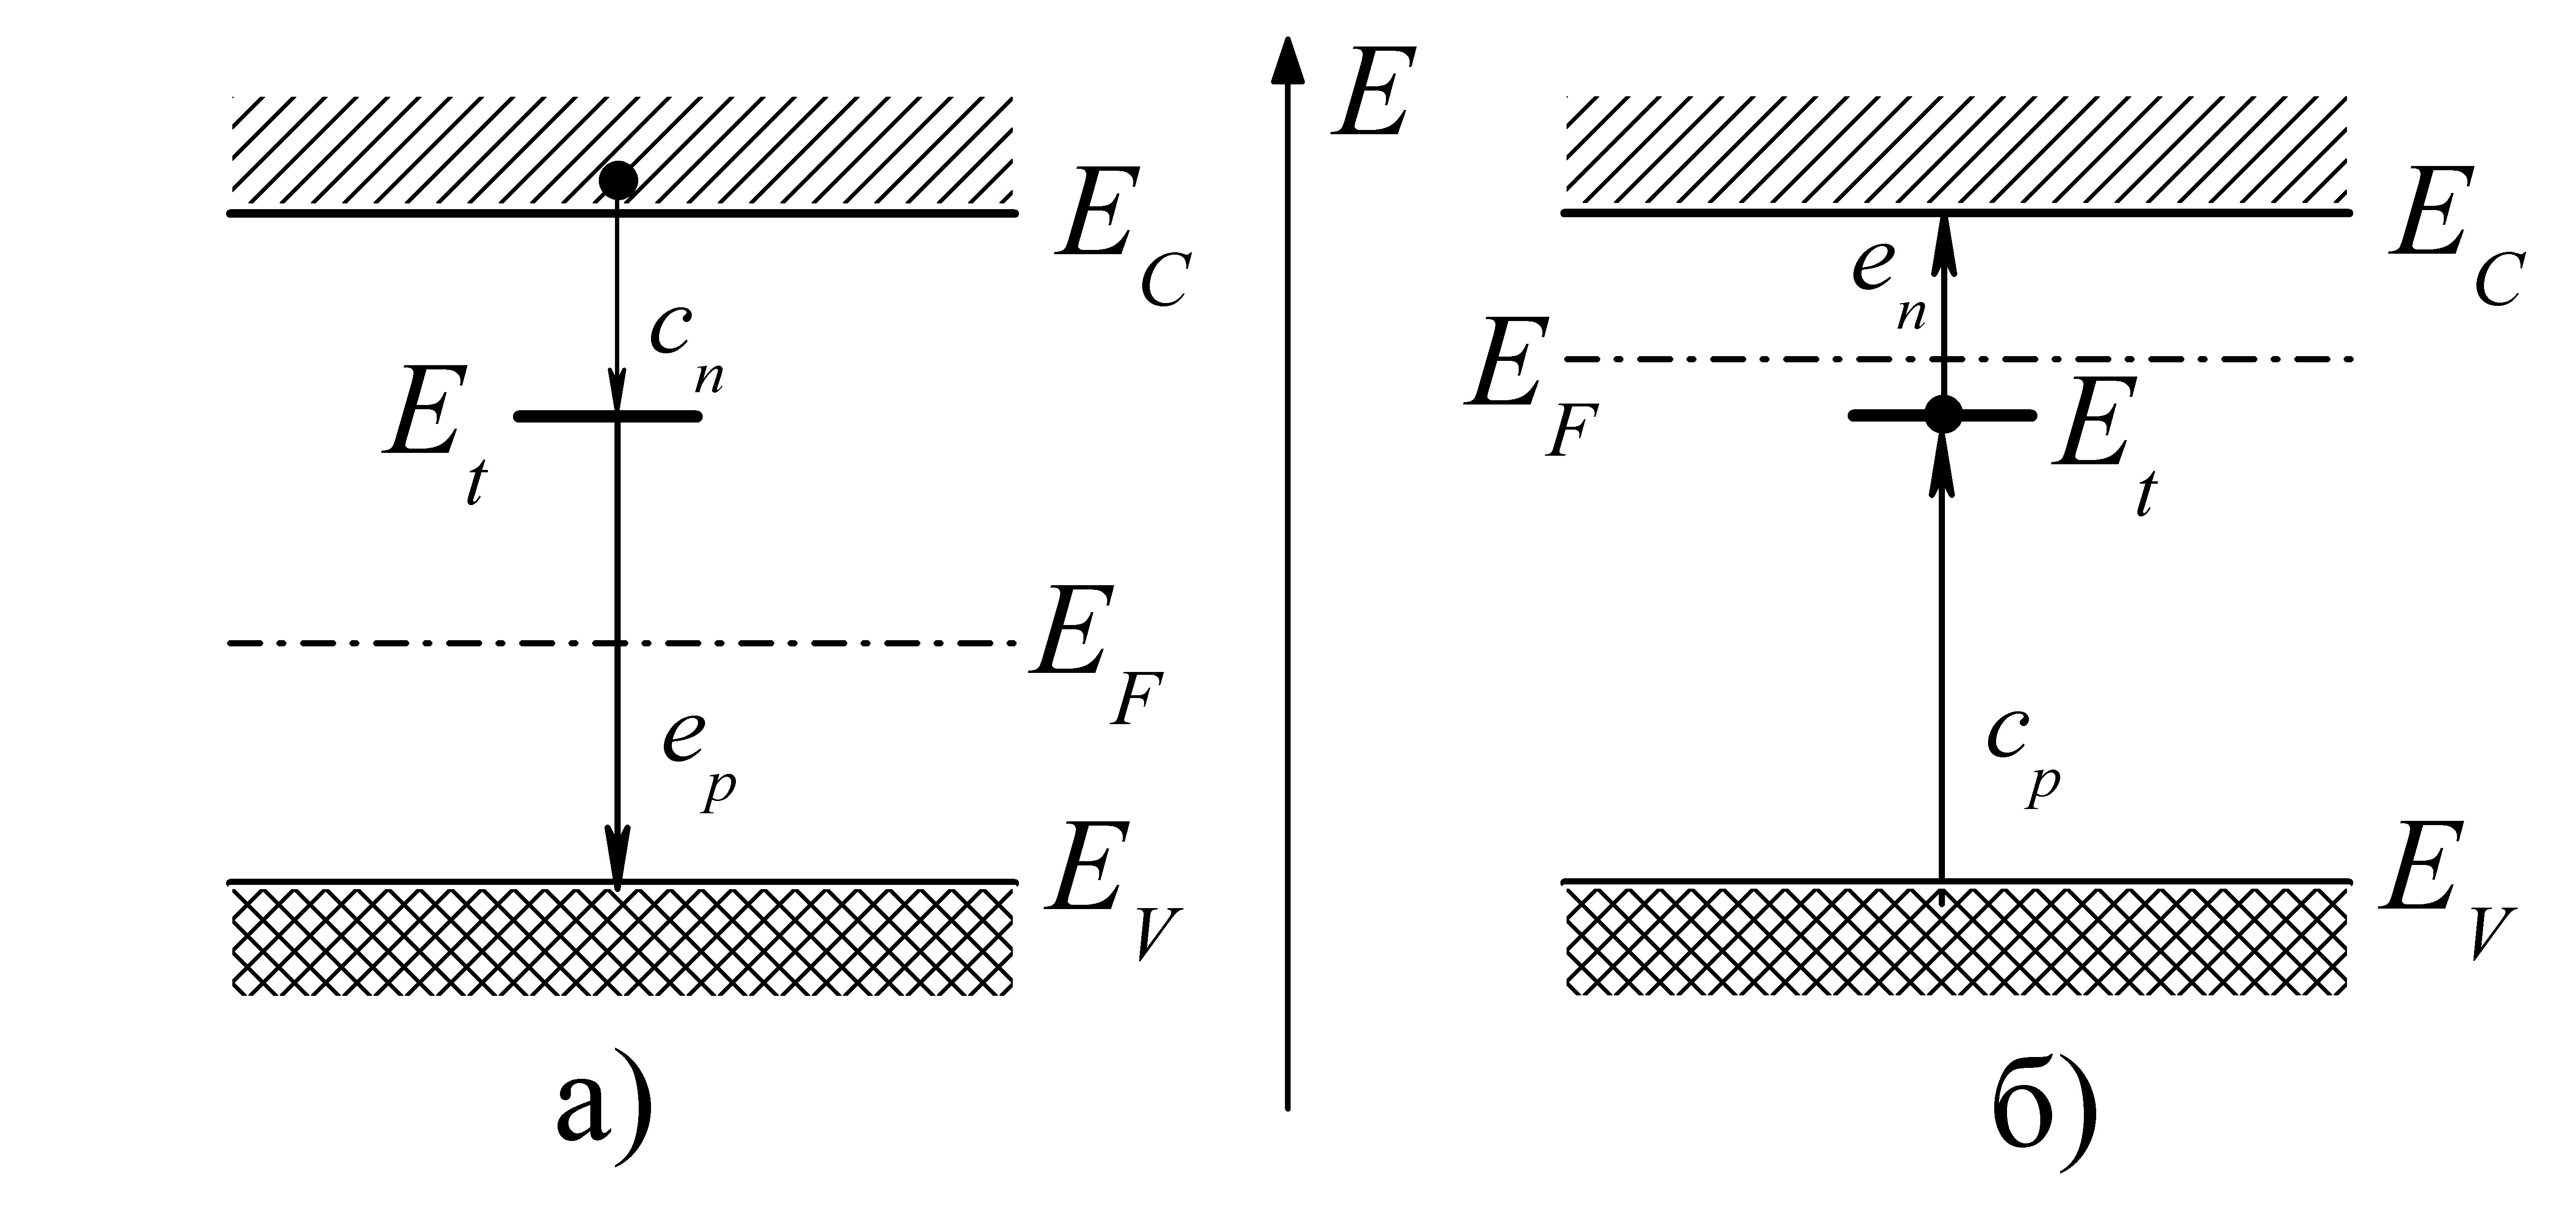
\includegraphics[width=0.4\textwidth]{Fig1_1}
\end{figure}
%
%
\begin{center}

{\scshape\bfseries Київ -- 2020}
\end{center}
\end{titlepage}
Б

УДК 004.7; 004.057.4.

\begin{center}

 \vspace{0.04\textheight}
 Рецензенти:
\end{center}
%\vspace{0.5cm}

\emph{С.В.~Кондратенко}, д-р. фіз.-мат. н., проф.

\emph{О.О.~Коротченков}, д-р. фіз.-мат. н., проф.

\vspace{1cm}
Рекомендовано до друку вченою радою фізичного факультету
Київського національного університету імені Тараса Шевченка
(протокол №10 від 18 квітня 2020 року)



\vspace{1cm}
\textbf{Оліх О.Я.}

Методи дослідження дефектів. Методичний посібник для студентів фізичного факультету. --- К.:2020.
%Іл.~236, табл.~51.

\vspace{1cm}
У посібнику розглянуто основні типи точкових дефектів, методи їх опису та термодинамічні підходи оцінки рівноважної концентрації.
Докладно викладено питання, які стосуються механізмів дифузії точкових дефектів.
Проаналізовано шляхи впливу на дефектну підсистему кристалів радіаційного опромінення і термічної обробки.
Наведено приклади найпоширеніших точкових комплексів у кремнії, а також розглянуто особливості метастабільних та бістабільних дефектів і центрів з від’ємною кореляційною енергією. Посібник містить задачі для самостійного розв’язання.            % Титульный лист

%\include{Dissertation/abstract}        % Анотація
%\include{Dissertation/abstractEn}        % Анотація

%\input{Dissertation/abstract}        % Анотація
%\input{Dissertation/abstractEn}        % Анотація

%\include{Dissertation/StatsAndAbst}

%\input{Dissertation/StatsAndAbst}

%\include{Dissertation/contents}        % Оглавление
%\chapter*{Перелік умовних скорочень та позначень}             % Заголовок
\addcontentsline{toc}{chapter}{Перелік умовних позначень та скорочень}  % Добавляем его в оглавление
\noindent
%\begin{longtabu} to \dimexpr \textwidth-5\tabcolsep {r X}
\begin{longtabu} to \textwidth {r X}
%  CDLR& coupled defect level recombination,  рекомбінація у системі спарених рівнів дефектів\\
  DLTS & deep--level transient spectroscopy, перехідна спектроскопія локальних рівнів\\
%  DAT & defect--assisted tunneling, тунелювання за участю рівнів дефектів \\
 % DE & differential evolution, метод диференційної еволюції \\%
%  FRC & fast--formed recombination center, швидко сформовані ВО дефекти \\
 % NIEL & non--ionizing energy losses, втрати, не пов'язані з іонізацією \\
%  MABC & modified artificial bee colony, метод  штучної бджолиної сім'ї\\
%  OSFR & oxidization induced stacking--faults ring, кільцеві дефекти пакування, що виникли при окисненні \\
%  PAT & phonon-assisted tunneling, стимулюване фононами тунелювання \\
%  PSO & particle swarm optimization, метод оптимізації зграї частинок\\
PAS & positron annihilation spectroscopy, позитронно--анігіляційна спектроскопія \\
%  RT & running time, час, необхідний для визначення параметрів\\
%  SCLC & space-charge limited current, струм, обмеженим просторовим зарядом \\
 % SRC & slow--formed recombination center, повільно сформовані ВО дефекти\\
%  TLBO & teaching learning based optimization, метод  оптимізованого викладання та навчання\\
%  VRHC &thermally-assisted variable-range-hopping conduction, термічно--активована стрибкова провідність зі змінною довжиною стрибка \\
%  AAД & акустоактивний дефект\\
%  АДВ & акусто--дефектна взаємодія \\
%  АІ & акусто--індукований\\
%  АХ & акустична хвиля\\
%  АЧХ & амплітудно--частотна характеристика\\
%  ВАХ & вольт--амперна характеристика\\
%  ВБШ & висота бар'єру Шотткі\\
%  ВТКС & високотемпературна компонента струму\\
%  ВФХ & вольт--фарадна характеристика\\
%  ГР &глибокий рівень \\
%  ДШ & діод Шотткі\\
%  ЕА & еволюційний алгоритм\\
%  КНО &  квазі--нейтральна область \\
%  КП & кисневмісні преципітати\\
%  КСЕ & кремнієвий сонячний елемент\\
%  MH & метал---напівпровідник \\
%  MОH & метал---окис---напівпровідник \\
%  МХО & мікро--хвильова обробка\\
%  НВЧ & надвисокочастотне \\
%  НТКС & низькотемпературна компонента струму\\
  ОПЗ & область просторового заряду \\
%  ПАН & поперечна акустоелектрична напруга\\
%  ПЕ & польова емісія\\
%  ППЗ & поперечний переріз захоплення \\
%  РД & радіаційний дефект \\
%  ТД &точковий дефект \\
%  ТЕ & термоелектронна емісія \\
%  ТПЕ & термопольова емісія \\
%  УЗ & ультразвук \\
%  УЗН & ультразвукове навантаження \\
%  УЗО & ультразвукова обробка \\
%  ШРХ & теорія Шоклі--Ріда--Хола  \\
$\alpha_+$ & коефіцієнт поглинання позитронів\\
$\alpha_{\sigma}$ & показник ступеня температурної залежності поперечного перерізу захоплення  \\
%$\alpha_R$ & температурний коефіцієнт опору\\
%$\alpha_\mathrm{\,FB}$ & температурний коефіцієнт ВБШ в наближені плоских зон\\
$\beta^+$ & позитрон  \\
%$\beta_1$, $\beta_2$  & коефіцієнти Варшні  \\
%$\Delta P$ & абсолютна АІ зміна параметра $P$\\
$\Delta C$ & надлишкова ємність безпосередньо після зміни прикладеної напруги\\
$\delta C$ & сигнал DLTS\\
$\gamma$ & гамма--квант \\
$\gamma_g$ & відношення кратностей виродження станів дефекту до та після захоплення електрону  \\
$\gamma_p$ & відношення кратностей виродження станів дефекту до та після захоплення дірки  \\
$\varepsilon$ & діелектрична проникність матеріалу  \\
$\varepsilon_0$ & діелектрична стала \\
%$\varepsilon_P$ & відносна AI зміна параметра $P$\\
%$\xi_\mathtt{cur}$ & відносна деформація приповерхневих кристалічних площин\\
%$\xi_\mathtt{US}$& амплітуда деформації ґратки при поширенні УЗ\\
%$\vartheta$ & темп генерації РД\\
%$\lambda$ &довжина хвилі падаючого світла\\
$\lambda_+$& темп анігіляції позитронів\\
$\lambda_{+,b}$& темп анігіляції позитронів у бездефектній області кристалу\\
$\lambda_{+,\mathrm{V}}$& темп анігіляції позитронів в околі вакансії\\
$\lambda_d$ & ширина області заряджених глибоких рівнів у ОПЗ\\
$\nu$ & частота падаючого світла \\
$\nu_e$& нейтрино \\
%%$\rho_\mathtt{LNO}$ & густина ніобату літію\\
%%$\rho_\mathtt{Si}$ & густина кремнію\\
$\rho_e$ & електронна густина\\
$\rho_N$ & концентрація ядер \\
$\varrho$&густина матеріалу\\
$\mu_t$ & коефіцієнт захоплення позитронів дефектом\\
%$\sigma_{\Phi0}$ & стандартне відхилення висоти бар'єру при нульовому зміщенні\\
$\sigma_{0}$& незалежний від температури множник у поперечному перерізі захоплення носіїв\\
$\sigma_{n(p)}$& поперечний переріз захоплення електронів (дірок) дефектом\\
%%$\sigma_p$& поперечний переріз захоплення дірок дефектом\\
$\tau_+$ & час життя позитронів\\
$\tau_{+,b}$& час життя позитронів у бездефектній області кристалу\\
$\tau_{+,\mathrm{V}}$& час життя позитронів у околі вакансії\\
$\left\langle\tau_+\right\rangle$ &середній час життя позитронів\\
%%$\tau$ & час релаксації заряду на пастках\\
%$\tau_{g}$ &ефективний час життя носіїв заряду в ОПЗ\\
%$\tau_{n}$ &ефективний час життя електронів\\
%$\tau_{n,\mathtt{RD}}$ & час життя електронів при рекомбінації на РД\\
%%$\upsilon_\mathtt{LNO}$ & швидкість звуку в ніобаті літію\\
$\upsilon_{th,n(p)}$& теплова швидкість електронів (дірок)\\
%%$\upsilon_{\mathrm{th},n}$ & теплова швидкість електронів\\
%%$\upsilon_{\mathrm{th},p}$ & теплова швидкість дірок\\
%%$\upsilon_\mathtt{Si}$ & швидкість звуку в кремнії\\
$\Phi_b$ & світловий потік\\
%$\Phi_b$ & ВБШ при нульовому зміщенні\\
%$\Phi_{b}^0$ & середнє значення ВБШ при нульовому зміщенні (ВБШ в однорідній області) \\
%$\Phi_{b}^\mathrm{FB}$ & ВБШ в наближені плоских зон \\
%$\Psi$ & флюєнс опромінення\\
$\psi_+$ & хвильова функція позитрону\\
%$\phi_0$ & рівень нейтральності інтерфейсних станів у структурі МН\\
%%$\zeta$ & диференційний показник нахилу ВАХ \\
%%$\omega_{ph}$ & частота фонону\\
%%$\omega_\mathtt{US}$ & циклічна частота АХ\\
%$A$ & площа зразка \\
%%$A_\mathtt{LNO}$ & площа п'єзоперетворювача\\
%$A^*$ & ефективна стала Річардсона \\
%%$a$ & стала ґратки \\
%%$a_B$ & радіус Бора\\
%%$B$ & коефіцієнт динамічної в'язкості \\
%%$b$ & модуль вектора Бюргерса \\
$C$ & ємність бар'єрної структури\\
$c$ & швидкість світла\\
$c_{n(p)}$ & швидкість захоплення вільних електронів (дірок) дефектом\\
$c_+$&швидкість захоплення позитронів дефектом \\
$c_{+,\mathrm{V}}$&швидкість захоплення позитронів дефектом вакансійного типу\\
%$D$ & доза опромінення\\
%%$D_d$ & displacement damage dose, ефективна доза, пов'язана з дефектоутворенням\\
%$D_{ss}$ & густина інтерфейсних станів у структурі МН\\
$d$ & ширина області спустошення дефектів в ОПЗ\\
$E$ & енергія електрону \\
$E_{+}$ & енергія позитрону\\
$E_{+,m}$ & максимальна енергія спектру позитронів\\
$E_{\sigma}$ & активаційна енергія поперечного перерізу захоплення \\
$E_C$ & енергія дна зони провідності \\
$E_D$ & положення енергетичного рівня донорної домішки\\
$E_G$ & ширина забороненої зони\\
$E_F$ & енергія Фермі\\
%$E_i$ & положення рівня Фермі у власному напівпровіднику\\
$E_t$ & положення енергетичного рівня, зв'язаного з дефектом\\
$E_{t+}$ & енергія позитронної іонізації дефекту\\
%$F\!F$ & фактор форми КСЕ\\
%$F_m$ & напруженість електричного поля на межі розділу МН \\
$E_V$ & енергія стелі валентної зони \\
$e^{-}$ & електрон \\
$e_+$ & швидкість емісії позитронів\\
$e_{n(p)}$ &швидкість термічної емісії електронів (дірок) дефектом\\
$e_n^o$& темп оптичної емісії електрону з глибокого рівня \\
%%$f_r$& резонансна частота п'єзоперетворювача\\
%$f_\mathtt{US}$& частота УЗ\\
$f_t$ & ймовірність заселеності електронного рівня\\
%%$G$ & модуль зсуву \\
$g$ & кратність квантовомеханічного виродження стану\\
$h$, $\hbar$ & стала Планка\\
$h^+$ & дірка\\
%$I$ & струм\\
%$I_s$ & струм насичення\\
%$I_R$ & зворотний струм\\
%%$J$ & густина струму\\
%$J_{ph}$ & густина фотогенерованого струму\\
%$J_{sc}$ & густина струму короткого замикання\\
$k$ & стала Больцмана\\
%$L_n$ & довжина дифузії електронів\\
$m_0$&маса спокою електрону\\
$m_+^*$& ефективна маса позитрону\\
$m_{n(p)}^*$ &  ефективна маса електрону (дірки)\\
$N_t$ & концентрація дефектів \\
$N_C$ & ефективна густина станів біля дна зони провідності\\
$N_D$ & концентрація донорів\\
%$N_d$ & концентрація електронів поблизу контакту МН\\
%$N_{t,\mathtt{RD}}$ & концентрація радіаційних дефектів\\
$N_V$ & ефективна густина станів біля вершини валентної зони\\
%$n_i$ & концентрація власних носіїв заряду\\
$n$ & концентрація електронів\\
$n_1$ &концентрація електронів у зоні провідності, коли рівень Фермі
співпадає з рівнем дефекту\\
$n_e$& кількість електронів в околі дефекту\\
%$n_\mathrm{id}$ & фактор неідеальності\\
%$n_{n(p)}$ & концентрація електронів у електронному (дірковому) напівпровіднику \\
%%$n_n$ & концентрація основних носіїв у електронному напівпровіднику \\
%%$n_p$ & концентрація неосновних носіїв у дірковому напівпровіднику \\
%%$q$ & елементарний заряд\\
$P_L$&ймовірність поглинання падаючої частинки при проходженні нею одиничного шляху\\
$p$ & концентрація дірок \\
$p^+(t)$ & частка  позитронів, які ще не проанігілювали в момент часу $t$\\
$p_{b}^+$ & частка вільних позитронів\\
$p_{t}^+$ & частка позитронів, захоплених дефектами\\
$p_{\mathrm{V}}^+$ & частка позитронів, захоплених дефектом вакансійного типу\\
$p_1$ &концентрація електронів у зоні провідності, коли рівень Фермі
співпадає з рівнем дефекту\\
%$p_{n(p)}$ & концентрація дірок у електронному (дірковому) напівпровіднику \\
%%$p_n$ & концентрація неосновних носіїв у електронному напівпровіднику \\
%%$p_p$ & концентрація основних носіїв у дірковому напівпровіднику \\
$Q^g$ & узагальнена координати\\
$Q$ & об'ємний заряд\\
$q$ & елементарний заряд\\
%%$R$ & темп рекомбінації \\
%%$R_\mathtt{cur}$ & радіус кривизни зразка \\
%$R_{\mathtt{DA}}$ & параметр зв'язку у моделі CDLR\\
%$R_{ph}$ & коефіцієнт відбивання світла\\
%$R_s$ & послідовний опір\\
%$R_{sh}$ & опір шунтування\\
$T$ & абсолютна температура\\
$T_{1/2}$ &період напіврозпаду \\
%$T_0$ & константа температурної залежності фактора неідеальності\\
%%$T_\mathtt{US}$ & період АХ\\
%%$t$ & час\\
$t_p$ & тривалість імпульсу заповнення\\
%$t_\mathtt{MWT}$ & час експозиції при МХО\\
%$t_\mathtt{UST}$ & час експозиції при УЗО\\
%$u_\mathtt{US}$&амплітуда зміщень атомів при поширенні УЗ\\
$V$ & напруга\\
$V_{bi}$ & контактна різниця потенціалів\\
%$V_{bb}$ & вигин зон напівпровідника поблизу контакту\\
%%$V_d$ & падіння напруги в околі бар'єру\\
%%$V_n$ & різниця потенціалів між дном зони провідності та положенням рівня Фермі в об'ємі напівпровідника\\
%$V_{oc}$ & напруга холостого ходу\\
%$V_R$ & зворотна напруга\\
%%$V_\mathtt{TAV}$ & величина ПАН\\
%$V_\mathtt{RF}$ & амплітуда напруги, прикладеної до п'єзоперетворювача\\
%%$V_v$ & об'єм кристалу\\
$W$ & ширина області просторового заряду \\
%$W_{ph}$ & інтенсивність освітлення \\
%$W_\mathtt{US}$ & інтенсивність акустичної хвилі\\

\end{longtabu}
\addtocounter{table}{-1}% Нужно откатить на единицу счетчик номеров таблиц, так как предыдующая таблица сделана для удобства представления информации по ГОСТ





        % Список сокращений и условных обозначений
%\include{Dissertation/introduction}    % Введение



\chapter{\MakeUppercase{Передумови та особливості використання активного ультразвука}}



\section{Ефекти впливу ультразвука на мікроелектронні структури та \\ матеріали \label{Oglyad}}
\cite{Olikh2019SM,Heide,Duan,n_CharGaN,n_CharSemic,n_CharPhysRevAppl,MachLean_RevModPhys,
MachLeanJAP,MachLeanPPV,SCRev2015,SCRev2020,FeB:Schmidt,IronSC,FeBLight2,FeB_Zong,
MurphyJAP2011,FeB:kinetic,FeBAssJAP2014,FeBKin2019,
ostapenko2002,Savkina2013,Olikh2018JAP,Davletova2008,Olikh2020JEM,Olikh:Ultras,OlikhJAP,Teterkin2009}:

%\cite{Sachenko2016,TAYYIB201221,FeB_Wilson,FeB_Walz,FeB_Zong,Breitenstein2013,SINKE2019,Wijaranakula,Narland,Sakauchi,Si_Auger,FeBLight,FeBLight2,FeB:Schmidt,FeBLight3,FeBCoDop,FeBDecay}

In the literature, there are several models that describe the current--voltage ($I-V$) characteristics of the solar cells (SCs).
These models contain some parameters, which reflect the processes within the structures and are related to the main characteristics of the photovoltaic conversion.
So single diode model with three parameters has been used to represent the SC static characteristic because of simplicity:
\begin{equation}
\label{eqIVs}
    I=I_{0}\left[\exp\left(-\frac{qV}{nkT}\right)-1\right]-I_{ph}\,,
\end{equation}
were









%\include{Dissertation/partSSC}

%\include{Dissertation/partMethodMS}

%\include{Dissertation/partGammaSD}


%\include{Dissertation/partUSL_T_SD}


%
\chapter{\MakeUppercase{Залишкові ефекти, спричинені мікрохвильовими та ультразвуковими обробками напівпровідникових структур на основі} GaAs, SiC ТА Si\label{Ch_UST_MW}}

\section{Вплив мікрохвильових обробок на дефектну підсистему структур GaAs та монокристалів карбіду кремнію}

Мікроелектроніка є однією з найважливіших галузей сьогодення і тому
вивчення впливу різноманітних зовнішніх факторів на властивості напівпровідників та структур на їхній основі є однією з найважливіших задач фізичного матеріалознавства.
Загалом цьому питанню присвячена значна кількість теоретичних та експериментальних робіт,
що викликано як бажанням зрозуміти механізми деградаційних процесів, які відбуваються у мікроелектронних приладах,
так і пошуком нових технологічних шляхів виготовлення таких пристроїв.
Вплив окремих факторів, наприклад радіації, вивчений достатньо повно --- див., наприклад, \cite{KorshunovBook,Kozlovs}.
Водночас більшої уваги починають потребувати нові засоби активного впливу, такі як, наприклад, УЗО чи мікрохвильова обробка (МХО) \cite{MW:Rev,Rjanov1981,paton1993,Vinnik1989,ZOHM2000,BHUNIA1998,Bacherikov2003r,Pashkov1994r,
Boltovets,Kr1996,Milenin1994,BelyaevIntac,ASHKINADZE1996,ProcSPIE,Venger1999,Belyaev1998JTFr,
Bacherikov2008,Konakova2015,Konakova2012FTP}.
В останньому випадку широке застосування надвисокочастотне (НВЧ) електромагнітне опромінення зумовлене його спроможністю викликати розігрів твердих тіл \cite{MW:Rev,ZOHM2000,paton1993}, причому визначальними особливостями такого підходу є висока ефективність, здатність як до однорідного, так і просторово--вибіркового підвищення температури та екстремально високі швидкості нагріву \cite{MW:Rev}.
Як наслідок, МХО широко використовується, для синтезу різноманітних, зокрема і напівпровідникових, сполук \cite{MW:Rev,BHUNIA1998}.
Проте подібний засіб зовнішнього впливу є також причиною зміни різноманітних характеристик напівпровідникових матеріалів та приладних структур.
Наприклад, виявлено, що НВЧ опромінення викликає релаксацію внутрішніх напруг та модифікацію приповерхневих
областей в структурах GaAs та InP \cite{Boltovets,Pashkov1994r,Kr1996,Milenin1994,BelyaevIntac,ProcSPIE,Venger1999,Konakova2015,Konakova2012FTP},
вирівнювання мікрорельєфу поверхні структур SiC/SiO$_2$ \cite{Bacherikov2003r},
перерозподіл домішок \cite{Bacherikov2003r,Belyaev1998JTFr,Konakova2015},
зміну зарядового стану комплексів \cite{Milenin1994}
та гетерування дефектів \cite{Belyaev1998JTFr}.
Одним із наслідків подібних процесів структурно--домішкового впорядкування є зменшення розкиду параметрів діодів Шотткі \cite{Milenin1994,Belyaev1998JTFr}.
Окрім того, спостерігалася стимульована НВЧ опроміненням
зміна властивостей плівок оксидів Ti, Gd та Er, осаджених на карбіді кремнію \cite{Bacherikov2008},
перебудова спектрів фотолюмінісценціїї пластин GaAs \cite{BelyaevIntac,ProcSPIE,Belyaev1998JTFr},
причому особливості ефекту залежали як від типу легуючої домішки, так і від кристалографічної орієнтації зразків.
Все це дозволяє розглядати МХО як один із найперспективніших, поряд із УЗО, шляхів модифікації напівпровідникових приладів.

Водночас детальніша інформація щодо впливу НВЧ опромінення на параметри глибоких центрів практично невідома.
Метою досліджень, результати яких наведено у цьому підрозділі є дослідження впливу МХО на параметри глибоких центрів, розташованих у приповерхневій області монокристалів $n$--6$H$--SiC та $n$--GaAs, а також арсенід--ґалієвих епітаксійних структур за допомогою методу акустоелектричної релаксаційної спектроскопії.



\subsection{Параметри структур та методи досліджень}

З літератури \cite{Boltovets,Kr1996,Milenin1994,BelyaevIntac,ASHKINADZE1996,ProcSPIE,Venger1999} відомо,
що загальний характер впливу МХО на напівпровідникові структури залежить від багатьох факторів; основними з них
є початковий рівень структурної досконалості, провідність, діелектрична проникність,топологія структур.
З метою оцінки впливу МХО на параметри відібрані різні (за ступенем легування, вихідним рівнем залишкових механічних напруг та структурою) зразки.
А саме.
\begin{enumerate}[label=\asbuk*),leftmargin=0em,itemindent=1.5em]
\item Монокристалічні пластини $n$--SiC, політип 6$H$, вирощені  за методом Лелі та леговані азотом.
Зразки мали вигляд пластин розміром $5\times10$~мм$^2$ товщиною 490~мкм із концентрацією носіїв $(3\div6)\cdot10^{18}$~см$^{-3}$ (надалі вони позначені SIC1 та SIC2)
і товщиною 460~мкм із концентрацією носіїв $(1\div3)\cdot10^{18}$~см$^{-3}$ (SIC3).

\item Монокристалічні пластини арсеніду ґалію товщиною 300~мкм.
Пластини орієнтовані в площині (100), леговані оловом, концентрація електронів дорівнювала $(1,5\div2,5)\cdot10^{18}$~см$^{-3}$ для зразка GAS1
та $(3\div5)\cdot10^{16}$~см$^{-3}$ для зразка GAS2.
Позначення GAT використовується для пластини (111), легованої телуром, $n=(1\div2)\cdot10^{18}$~см$^{-3}$.

\item Епітаксійні $n$--$n^+$ структури GaAs, які складалися з монокристалічної підкладки товщиною 300~мкм із $n=2\cdot10^{18}$~см$^{-3}$
та нанесеного на його поверхню  шару товщиною 6~мкм із концентрацією носіїв $3,9\cdot10^{15}$~см$^{-3}$ (зразок GAE1),
$3,5\cdot10^{15}$~см$^{-3}$ (GAE2), $5,0\cdot10^{15}$~см$^{-3}$ (GAE3).
Підкладка та епітаксійний шар леговані телуром.

\item Епітаксійні $n$--$n^+$--$n^{++}$ структури GaAs:Te з буферним шаром, які складалися з монокристалічної (100) підкладки (300~мкм, $n=2\cdot10^{18}$~см$^{-3}$),
на яку послідовно нанесені шар товщиною 1~мкм з $n=8\cdot10^{16}$~см$^{-3}$
та шар товщиною 2~мкм, у якому $n=7\cdot10^{15}$~см$^{-3}$.
Для досліджень використовувалися зразки, вирізані з двох різних пластин та позначені GAB1 та GAB2.
\end{enumerate}
Епітаксійні системи  виготовлені за допомогою методу газофазної епітаксії і відповідали стандартним технічним умовам на подібні структури.
Використані зразки узагальнені на рис.~\ref{figSamp_TAV}.

\begin{figure}
\center
\includegraphics[width=0.95\textwidth]{figSamp_TAV}
\caption{\label{figSamp_TAV}
Структура зразків для вивчення глибоких рівнів}%
\end{figure}

МХО зразків проводилася у вільному просторі при кімнатній температурі в магнетроні на частоті 2,45 ГГц із питомою потужністю  $1,5$~Вт/см$^2$.
Опромінення епітаксійних структур здійснювалося з боку розташування епітаксійного шару.
Загальний час експозиції $t_\mathtt{MWT}$ змінювався в інтервалі $20\div80$~c для різних зразків.
З метою запобігання суттєвого нагріву зразків тривалість неперервного опромінення складала 5~с.

До та після МХО визначалися такі параметри глибоких центрів, як ефективний поперечний переріз захоплення електронів $\sigma_n$
та розташування енергетичного рівня центру відносно дна зони провідності $E_c-E_t$.
Для цього використовувався метод акустоелектричної релаксаційної спектроскопії \cite{Saiko1993,OstrovPAN,OlikhSSC},
який вже згадувався у пункті~\ref{secUSMethod}.
Схема методу зображена на рис.~\ref{figTAV}.
Зразки розміщувалися на п'єзоелектричній пластині LiNbO$_3$, в якій імпульсно збуджувалися АХ.
%Поширення УЗ в пластині супроводжується електричним полем, яке проникало в напівпровідник.
%Внаслідок акусто--електронної взаємодії в напівпровіднику виникає постійна напруга, пов'язана з перерозподілом носіїв заряду,
%захоплених пастками, розташованими в приповерхневому шарі --- так звана поперечна акустоелектрична напруга (ПАН).
Після закінчення УЗ імпульсу відбувається релаксація ПАН згідно з законом
\begin{equation}\label{eqVtav}
  V_\mathtt{TAV}(t)=V_{\mathtt{TAV},0}\exp(-t/\tau).
\end{equation}

\begin{figure}
\center
\includegraphics[width=0.8\textwidth]{figTAV}
\caption{\label{figTAV}
Схема вимірювання сигналу ПАН.
Схематично показано часові залежності радіоімпульсу $V_\mathtt{RF}$ для збудження УЗ в пластині п'єзоелектрика
та результуючого сигналу ПАН $V_\mathtt{TAV}$.
}%
\end{figure}

Проста експоненційна залежність (\ref{eqVtav}) спостерігається у випадку, коли у акустоелектронній взаємодії ефективно приймають участь глибокі центри лише одного типу.
Для електронного напівпровідника характерний час релаксації описується співвідношенням \cite{Saiko1993,Rzanov,OstrovPAN}
\begin{equation}\label{eqPANtau}
  \tau=\frac{1}{\sigma_n\,\upsilon_{\mathrm{th},n}\,N_c}\exp\left(\frac{E_c-E_t}{kT}\right).
\end{equation}
Експериментальні вимірювання релаксаційної ділянки ПАН при різних температурах та їхня подальша апроксимація згідно з (\ref{eqVtav}) дозволяли отримати
залежність $\tau(T)$.
Величина $E_c-E_t$ визначалася за нахилом залежності $\tau$ від $(kT)^{-1}$ у напівлогарифмічному масштабі, після чого, з використанням формули (\ref{eqPANtau}),
був розрахований $\sigma_n$.
Виміри проводилися в інтервалі температур (290$\div$350)~К,
за винятком зразків GAB, для який ПАН досягала достатньої для вимірювання величини лише після нагріву до температур вище 310~К.

Для монокристалічних зразків до та після МХО також проведено визначення радіуса кривизни $R_\mathtt{cur}$ та
деформації $\xi_\mathtt{cur}$ приповерхневих кристалографічних площин.
Величина $\xi_\mathtt{cur}$ оцінювалася рентгенографічним методом по зміні кутового положення дифракційного максимуму при трансляції зразка \cite{Godwod},
кривизна вимірювалася на профілометрі DekTak 3030 Veeco Instruments.
$R_\mathtt{cur}$ та $\xi_\mathtt{cur}$ вимірювалися  з відносною похибкою, що не перевищувала 2~\%.
Для монокристалів арсеніду ґалію досліджувався також характер розподілу структурних дефектів по площі за допомогою методу
рентгенівської проекційної топографії за Борманом,
а розподіл густини дислокацій та мікронапруг визначався методом аналізу інтенсивності фріделівських пар відбиттів $hkl$ та $hk\overline{l}$ \cite{ThoricBook}.


\subsection{Вплив мікрохвильових обробок на параметри глибоких рівнів}

На рис.~\ref{figTauTAV} наведено типові температурні залежності $\tau$ для зразків до та після МХО.
З наведених даних видно, що після дії НВЧ опромінення змінюється як нахил кривих (безпосередньо пов'язаний
з розташуванням рівня у забороненій зоні), так і абсолютна величина характерного часу релаксації ПАН.
Характер та величина впливу залежать як від часу експозиції, так і від ступеня легування та внутрішньої будови
досліджених структур.
Отримані результати узагальнені в табл.~\ref{tabMW}.
Видно, що в зразках карбіду кремнію зустрічається 2 глибокі рівні, позначені ESC1 та ESC2,
в зразках арсеніду ґалію --- шість (EGA1--EGA6).


\begin{figure}
\center
\includegraphics[width=0.99\textwidth]{figTauTAV}
\caption{\label{figTauTAV}
Залежності часу релаксації ПАН від оберненої температури для
зразків SIC2 (а), SIC3 (б), GAS2 (в), GAE2 (г) та GAB1 (д) до та після МХО.
$t_\mathtt{MWT}$, c: 0 (криві 1), 20 (2), 40 (3), 60 (4)
}%
\end{figure}

\begin{table}
\caption{\label{tabMW}Визначені параметри дефектів у зразках $n$--GaAs та $n$--6$H$--SiC
}
\center
\renewcommand{\arraystretch}{0.95}
\begin{tabular}{|c|c|c|c|c|c|c|}
\hline
%Зразок& $t_\mathtt{MWT}$, c & $(E_c-E_t)$, еВ &$\sigma_n$, см$^2$\textsuperscript{ a)}&$R_\mathtt{cur}$, м&$\xi_\mathtt{cur}$\\
Зразок& $t_\mathtt{MWT}$, c &Рівень &$(E_c-E_t)$, еВ &$\sigma_n$, см$^2$\textsuperscript{ a)}&$R_\mathtt{cur}$, м&$\xi_\mathtt{cur}$\\
\hhline{|=======|}
SIC1& 0 &ESC1& $0,33\pm0,01$ &$(7\pm4)\cdot10^{-18}$&$\infty$&0\\ \cline{2-7}
& 20 &ESC1& $0,33\pm0,01$ &$(5\pm3)\cdot10^{-19}$&170,2&$8,7\cdot10^{-7}$\\ \cline{2-7}
& 40 &ESC2& $0,26\pm0,01$ &$(2\pm1)\cdot10^{-19}$&\multicolumn{2}{c|}{\multirow{2}{*}{н/в}}\\ \cline{2-5}
& 80 & \multicolumn{3}{c|}{c/c}&\multicolumn{2}{c|}{}\\ \hline
SIC2& 0 &ESC1& $0,33\pm0,01$ &$(7\pm4)\cdot10^{-18}$&$>2000$&$<1,2\cdot10^{-7}$\\ \cline{2-7}
& 20 &ESC1& $0,33\pm0,01$ &$(5\pm3)\cdot10^{-19}$&171,9&$1,4\cdot10^{-6}$\\ \hline
SIC3& 0 &ESC1& $0,34\pm0,02$ &$(3\pm2)\cdot10^{-18}$&3,8&$6,1\cdot10^{-5}$\\ \cline{2-7}
& 20 &ESC2&$0,29\pm0,01$ &$(5\pm3)\cdot10^{-19}$&5,5&$4,2\cdot10^{-5}$\\ \cline{2-7}
& 40 &ESC2& $0,26\pm0,01$ &$(10\pm7)\cdot10^{-20}$&\multicolumn{2}{c|}{\multirow{2}{*}{н/в}}\\ \cline{2-5}
& 80 &ESC2& $0,23\pm0,01$ &$(6\pm4)\cdot10^{-20}$&\multicolumn{2}{c|}{}\\ \hline
GAS1& 0 &EGA1& $0,32\pm0,02$ &$(3\pm2)\cdot10^{-17}$&-53,8&$-2,8\cdot10^{-6}$\\ \cline{2-7}
& 20 &EGA1& $0,31\pm0,01$ &$(2\pm1)\cdot10^{-17}$&22,9&$6,5\cdot10^{-6}$\\ \cline{2-7}
& 40 & \multicolumn{3}{c|}{c/c}&\multicolumn{2}{c|}{н/в}\\ \hline
GAS2& 0 &EGA1& $0,32\pm0,01$ &$(4\pm2)\cdot10^{-17}$&17,2&$8,7\cdot10^{-6}$\\ \cline{2-7}
& 20 &EGA2& $0,28\pm0,01$ &$(5\pm2)\cdot10^{-18}$&14,7&$1,0\cdot10^{-5}$\\ \cline{2-7}
& 40 & \multicolumn{3}{c|}{c/c}&\multicolumn{2}{c|}{}\\ \cline{1-5}
GAT& 0 &EGA3& $0,49\pm0,02$ &$(5\pm3)\cdot10^{-14}$&\multicolumn{2}{c|}{}\\ \cline{2-5}
& 20 &EGA4& $0,40\pm0,02$ &$(2\pm1)\cdot10^{-15}$&\multicolumn{2}{c|}{}\\ \cline{1-5}
GAE1& 0 &EGA5& $0,24\pm0,01$ &$(2\pm1)\cdot10^{-18}$&\multicolumn{2}{c|}{}\\ \cline{2-5}
& 60 &EGA2& $0,29\pm0,01$ &$(10\pm6)\cdot10^{-18}$&\multicolumn{2}{c|}{}\\ \cline{1-5}
GAE2& 0 &EGA5& $0,25\pm0,01$ &$(2\pm1)\cdot10^{-18}$&\multicolumn{2}{c|}{}\\ \cline{2-5}
& 60 &EGA2& $0,30\pm0,01$ &$(2\pm1)\cdot10^{-17}$&\multicolumn{2}{c|}{}\\ \cline{1-5}
GAE3& 0 &EGA6& $0,43\pm0,01$ &$(8\pm5)\cdot10^{-17}$&\multicolumn{2}{c|}{н/в}\\ \cline{2-5}
& 60 &EGA6& $0,46\pm0,02$ &$(7\pm4)\cdot10^{-16}$&\multicolumn{2}{c|}{}\\ \cline{1-5}
GAB1& 0 &EGA4& $0,39\pm0,01$ &$(10\pm7)\cdot10^{-18}$&\multicolumn{2}{c|}{}\\ \cline{2-5}
& 20 &EGA4& $0,39\pm0,01$ &$(4\pm2)\cdot10^{-17}$&\multicolumn{2}{c|}{}\\ \cline{2-5}
& 40 &EGA6& $0,43\pm0,02$ &$(10\pm6)\cdot10^{-17}$&\multicolumn{2}{c|}{}\\ \cline{1-5}
GAB2& 0 &EGA4& $0,40\pm0,01$ &$(10\pm6)\cdot10^{-17}$&\multicolumn{2}{c|}{}\\ \cline{2-5}
& 20 &EGA4& $0,41\pm0,01$ &$(10\pm6)\cdot10^{-17}$&\multicolumn{2}{c|}{}\\ \cline{2-5}
& 40 &EGA6& $0,45\pm0,02$ &$(4\pm2)\cdot10^{-16}$&\multicolumn{2}{c|}{}\\  \hline
\multicolumn{6}{l}{\textsuperscript{ a)} \emph{при $T=300$~К для SIC, GA, GAE та при  $T=340$~К для GAB}}\\
\multicolumn{6}{l}{\emph{н/в --- вимірювання не проводилися; с/с --- слабкий сигнал ПАН}}\\
%\multicolumn{6}{l}{\emph{с/с --- величина ПАН недостатня для визначення параметрів пасток}}\\
\end{tabular}
\end{table}

Для наведених даних є характерною низка особливостей.
А саме.
\begin{enumerate}[label=\arabic*),leftmargin=0em,itemindent=1.5em]
\item Величина перерізу захоплення носіїв значно чутливіша до МХО, ніж енергетичне розташування рівнів.
Наприклад, виявлено зміни $\sigma_n$ на порядок величини, тоді як зміщення положення рівнів не перевищує 20\%;
крім того, модифікація перерізу захоплення спостерігається при менших часах експозиції: так, наприклад,
для GAB1 після 20~с НВЧ впливу значення $(E_c-E_t)$ практично не змінилося, тоді як $\sigma_n$ зросла приблизно в чотири рази.

\item У монокристалах ступінь індукованих МХО змін зростає при зменшенні концентрації вільних носіїв заряду (див. дані для зразків GAS1 та GAS2) та зростанні відносної деформації (зменшенні кривизни поверхні).

\item Після тривалої (для GaAs $t_\mathtt{MWT}\geq40$~с, для SiC $t_\mathtt{MWT}\geq80$~с) МХО монокристалічних
зразків спостерігається суттєве зменшення сигналу ПАН.
Це корелює з даними роботи \cite{Belyaev1998JTFr}, де повідомляється про зменшення концентрації центрів із
рівнями у верхній половині забороненої зони внаслідок НВЧ відпалу.

\item Доза опромінення, необхідна для суттєвого впливу на параметри центрів у епітаксійних структурах, вища, ніж
для монокристалічних зразків.
Зокрема про це свідчать дані табл.~\ref{tabMW} для зразків серій GA та GAB після опромінення протягом 20~с.
Зауважимо, що рівень легування підкладки GAB та GAE збігався зі зразками GAS1 і GAT,
епітаксійного шару GAB --- з GAS2;
крім того, в GAB, GAE та GAT однакова легуюча домішка.
Відтак, виявлені відмінності визначаються структурою зразків, а не зумовлені різницею їхніх провідностей.

\item Характер змін у монокристалічних пластинах та епітаксійних структурах протилежний:
для SIC, GAS, GAT після МХО спостерігається зменшення $\sigma_n$ та $(E_c-E_t)$, тоді як в GAE та GAB обидва параметри зростають.
\end{enumerate}

Спираючись відомі дані, розглянемо можливу природу центрів,
які виявлені у досліджених структурах.
При цьому необхідно врахувати, що літературні дані характеризуються наявністю розкиду значень основних параметрів
пасток, зокрема відмінності величини поперечного перерізу захоплення можуть досягати чотирьох порядків \cite{Pavlovic2000}.
Однією з можливих причин цього феномену може бути суттєва залежність швидкості термічної емісії носіїв від
напруженості електричного поля  \cite{Bulyarskii2000r,Makram,Shishiyanu},
яка викликана
а)~зменшенням енергії іонізації внаслідок ефекту Пула--Френкеля чи, наприклад,
завдяки кулонівській взаємодії центрів \cite{Stellmacher};
б)~зміною величини $\sigma_n$ \cite{Shishiyanu,Bourgoin2001}.
Зазвичай зміни $(E_c-E_t)$ складають декілька сотих еВ, тоді
зміни перерізу захоплення можуть досягати декількох порядків:
наприклад, згідно з даними роботи \cite{Bourgoin2001}  при кімнатній температурі $\sigma_n$ для центру EL2 в GaAs при напруженості $10^5$~В/см збільшується в 200 разів.
Як наслідок, при використанні різних методів дослідження дефектів отримані параметри одних і тих же центрів
можуть суттєво відрізнятися.
Наприклад, можна порівняти результати оглядових робіт, де зібрані дані по різноманітним пасткам в арсеніді ґалію отримані за допомогою методів нестаціонарної емнісної спектроскопії \cite{Bourgoin:GaAs} та
термостимульованих струмів \cite{Pavlovic2000}.
Наведені дані стосуються дефектів із близьким положенням рівнів і суттєво різними значеннями поперечного перерізу захоплення.
Узагальнюючи сказане, зауважимо, що при ідентифікації дефектів будемо орієнтуватися саме на енергетичне розташування
пасткових рівнів.


Положення рівня ESC1 ($E_c-(0,33\div0,34)$~еВ), який спостерігався у вихідних монокристалах карбіду кремнію
можна зіставити з розташуванням $S$--центру ($E_c-0,35)$~еВ, \cite{Lebed1999,Anikin1991:2,Anikin1991:3}),
$EK3$--центру ($E_c-0,34)$~еВ, \cite{Kuznets1997}) чи рівня $(-/+)$ центру $E_1$ ($E_c-0,34)$~еВ, \cite{Lebed1999}).
$S$--центр відповідає за безвипромінювальну рекомбінацію і відноситься до власних дефектів у 6$H$--SiC \cite{Lebed1999}).
Згідно з результатами робіт \cite{Anikin1991:2,Anikin1991:3} $S$--центр та $R$--центр ($E_c-1,27$~еВ) пов'язані
з двома різними зарядовими станами одного й того ж дефекту, тоді як відповідно до даних роботи \cite{Lebedev2000}
$R$--центр є дивакансією V$_\text{Si}$V$_\text{C}$.
З рівнем $E_1$, який є центром із від'ємною кореляційною енергією,
пов'язують комплекс кремнієвих вакансій  \cite{Lebedev2001}.
Після МХО розташування рівня, що відповідає за появу ПАН в SIC, змінюється до $E_c-(0,26\div0,29)$~еВ (рівень ESC2).
При цьому також немає повної однозначності:
близьке положення має рівень донорний рівень $(0/+)$ центру $E_1$ ($E_c-(0,27\div0,28)$~еВ, \cite{Hemmingsson})
та центр $X_1$ ($E_c-0,3$~еВ, \cite{Lebedev2001}).
Автори останньої роботи доповідають про суттєву залежність концентрації $X_1$ від структурної
досконалості кристалу та підкреслюють не ідентичність цього центру  з  $E_1$.

%Інформація  для центрів у  арсеніді ґалію розглянута в літературі значно ширше.
Дані для кожного з виявлених рівнів у  арсеніді ґалію узагальнено в таблицях~\ref{tabEGA1}--\ref{tabEGA6}.
Наведені дані показують, що виявлені центри пов'язані з власними дефектами вакансійного типу.

\begin{table}
\caption{\label{tabEGA1}Літературні дані для рівнів, близьких за розташуванням до EGA1
($E_c-E_t=(0,31\div0,32)$~еВ, $\sigma_n\approx3\cdot10^{-17}$~см$^2$, зразки GAS1 та GAS2)
}
\center
\begin{tabular}{|c|c|c|c|c|c|}
\hline
$(E_c-E_t)$, еВ &$\sigma_n$, см$^2$&конфігурація&метод&епі--структура&посилання\\ \hline
0,33&&комплекс з V$_\text{As}$&DLTS&ні&\cite{EL6:Richter}\\ \hline
0,33&&&DLTS&ні&\cite{Neild1991}\\ \hline
$0,31\div0,33$&&V$_\text{As}$&&&\cite{EL6:Schultz}\\ \hline
0,33&$1\cdot10^{-17}$&&TSC&ні&\cite{Pavlovic2000}\\ \hline
0,323&$1\cdot10^{-14}$&&DLTS&так&\cite{Yousefi1995}\\ \hline
0,334&$2\cdot10^{-15}$&&DLTS&так&\cite{Yousefi1995}\\ \hline
0,35&&комплекс з V$_\text{As}$&PA&ні&\cite{EL6:Kuisma}\\ \hline
$0,315\div0,325$&$3\cdot10^{-17}$&&TSC&ні&\cite{Pavlovic:GaAs}\\ \hline
0,33&&&TSC&ні&\cite{Tomozane:GaAs}\\ \hline
$0,30\div0,33$&&&DLTS&ні&\cite{Lang:GaAs}\\ \hline
\multicolumn{6}{l}{ \emph{DLTS --- метод нестаціонарної спектроскопії ГР}}\\
\multicolumn{6}{l}{ \emph{TSC --- метод термостимульованих струмів}}\\
\multicolumn{6}{l}{ \emph{PA --- позитрон--анігіляційна спектроскопія}}\\
\end{tabular}
\end{table}


\begin{table}
\caption{\label{tabEGA2}Літературні дані для рівнів, близьких за розташуванням до EGA2
($E_c-E_t=(0,31\div0,32)$~еВ, $\sigma_n\approx5\cdot10^{-18}$~см$^2$ (монокристали),
$1\cdot10^{-17}$~см$^2$ (епі-структури), зразки GAS2, GAE1 та GAE2 після опромінення)
}
\center
\begin{tabular}{|c|c|c|c|c|c|}
\hline
$(E_c-E_t)$, еВ &$\sigma_n$, см$^2$&конфігурація&метод&епі--структура&посилання\\ \hline
0,28&$5\cdot10^{-18}$&V$_\text{As}$As$_i$&TSC&ні&\cite{Pavlovic2000}\\ \hline
0,26&$3,5\cdot10^{-15}$&&DLTS&так&\cite{Yousefi1995}\\ \hline
$0,277$&$5\cdot10^{-17}$&&TSC&ні&\cite{Pavlovic:GaAs}\\ \hline
$0,284$&$1\cdot10^{-17}$&&TSC&ні&\cite{Pavlovic:GaAs}\\ \hline
0,28&&власний&TP&ні&\cite{Abele:GaAs}\\ \hline
0,28&$8\cdot10^{-15}$&&DLTS&так&\cite{Mircea1975}\\ \hline
0,30&&комплекс з Те&DLTS&ні&\cite{KolFTP1994r}\\ \hline
0,30&$6\cdot10^{-15}$&V$_\text{As}$As$_i$&DLTS&ні&\cite{Pons}\\ \hline
\multicolumn{6}{l}{\emph{TP --- релаксація фотопровідності}}\\
\end{tabular}
\end{table}



\begin{table}
\caption{\label{tabEGA3}Літературні дані для рівнів, близьких за розташуванням до EGA3
($E_c-E_t=0,49$~еВ, $\sigma_n\approx5\cdot10^{-14}$~см$^2$, зразок GAТ)
}
\center
\begin{tabular}{|c|c|c|c|c|c|}
\hline
$(E_c-E_t)$, еВ &$\sigma_n$, см$^2$&конфігурація&метод&епі--структура&посилання\\ \hline
0,50&&Sb$_\text{Ga}$&DLTS&ні&\cite{Samoilov1994}\\ \hline
0,48&$4\cdot10^{-16}$&As$_\text{Ga}^{++}$&TSC&ні&\cite{Pavlovic2000}\\ \hline
$0,485$&$2\cdot10^{-16}$&&TSC&ні&\cite{Pavlovic:GaAs}\\ \hline
$0,48$&&домішка&TP&ні&\cite{Abele:GaAs}\\ \hline
0,51&$1\cdot10^{-12}$&&DLTS&ні&\cite{Martin1977}\\ \hline
0,48&$3\cdot10^{-13}$&&DLTS&ні&\cite{Lang:GaAs}\\ \hline
0,50&$1\cdot10^{-15}$&V$_\text{As}$, V$_\text{Ga}$Ga$_i$V$_\text{As}$ &DLTS&ні&\cite{Pons}\\ \hline
\end{tabular}
\end{table}

\begin{table}
\caption{\label{tabEGA4}Літературні дані для рівнів, близьких за розташуванням до EGA4
($E_c-E_t=(0,39\div0,41)$~еВ, $\sigma_n\approx2\cdot10^{-15}$~см$^2$ (монокристали),
$(1\div10)\cdot10^{-17}$~см$^2$ (епі-структури), зразки GAТ та GAB)
}
\center
\begin{tabular}{|c|c|c|c|c|c|}
\hline
$(E_c-E_t)$, еВ &$\sigma_n$, см$^2$&конфігурація&метод&епі--структура&посилання\\ \hline
0,42&&&DLTS&ні&\cite{Neild1991}\\ \hline
0,41&&V$_\text{Ga}$V$_\text{As}$&DLTS&ні&\cite{Samoilov1994}\\ \hline
$0,39$&&V$_\text{Ga}$Ga$_\text{As}$&TSC&ні&\cite{FANG1990}\\ \hline
$0,41$&$2\cdot10^{-13}$&&DLTS&так&\cite{Bourgoin:GaAs}\\ \hline
0,40&&&SCRC&так&\cite{ASHBY:GaAs}\\ \hline
0,37&$2\cdot10^{-14}$&&DLTS&так&\cite{Fang:EL6}\\ \hline
0,40&&V$_\text{Ga}$Ga$_\text{As}$&DLTS&ні&\cite{Vaitkus}\\ \hline
0,387&$2\cdot10^{-14}$&&DLTS&так&\cite{Yousefi1995}\\ \hline
\multicolumn{6}{l}{\emph{SCRC --- температурна залежність струму ОПЗ}}\\
\end{tabular}
\end{table}



\begin{table}
\caption{\label{tabEGA5}Літературні дані для рівнів, близьких за розташуванням до EGA5
($E_c-E_t=(0,24\div0,25)$~еВ, $\sigma_n\approx2\cdot10^{-18}$~см$^2$, зразки GAE1 та GAE2 до опромінення)
}
\center
\begin{tabular}{|c|c|c|c|c|c|}
\hline
$(E_c-E_t)$, еВ &$\sigma_n$, см$^2$&конфігурація&метод&епі--структура&посилання\\ \hline
0,23&&&DLTS&ні&\cite{Neild1991}\\ \hline
0,23&$2\cdot10^{-17}$&&TSC&ні&\cite{Pavlovic2000}\\ \hline
$0,22\div0,25$&$8\cdot10^{-19}$&&TSC&ні&\cite{Lin:GaAs}\\ \hline
$0,26$&&комплекс з V$_\text{Ga}$&TSC&ні&\cite{FANG1990}\\ \hline
0,24&&&TSC&ні&\cite{Tomozane:GaAs}\\ \hline
0,23&&власний&TP&ні&\cite{Abele:GaAs}\\ \hline
0,23&&V$_\text{Ga}$V$_\text{As}$&DLTS&ні&\cite{Morrow:EL17}\\ \hline
0,23&$1\cdot10^{-14}$&V$_\text{Ga}$V$_\text{As}$&DLTS&ні&\cite{Bourgoin:GaAs}\\ \hline
0,23&$7\cdot10^{-15}$&&DLTS&так&\cite{Mircea1975}\\ \hline
0,22&$2\cdot10^{-15}$&&DLTS&ні&\cite{Fang:EL6}\\ \hline
0,258&$4\cdot10^{-16}$&&DLTS&так&\cite{Yousefi1995}\\ \hline
\end{tabular}
\end{table}



\begin{table}
\caption{\label{tabEGA6}Літературні дані для рівнів, близьких за розташуванням до EGA6
($E_c-E_t=(0,43\div0,46)0,43$~еВ, $\sigma_n\approx8\cdot10^{-17}$~см$^2$ (GAE3 до опромінення)
$\sigma_n\approx5\cdot10^{-16}$~см$^2$ (GAE3, GAB після опромінення))
}
\center
\begin{tabular}{|c|c|c|c|c|c|}
\hline
$(E_c-E_t)$, еВ &$\sigma_n$, см$^2$&конфігурація&метод&епі--структура&посилання\\ \hline
0,44&$1\cdot10^{-14}$&V$_\text{As}$As$_i$, V$_\text{As}$&TSC&ні&\cite{Pavlovic2000}\\ \hline
0,44&$9\cdot10^{-15}$&&TSC&ні&\cite{Pavlovic:GaAs}\\ \hline
$0,43$&$7\cdot10^{-16}$&власний&DLTS&так&\cite{Lefevre1977,Bourgoin:GaAs}\\ \hline
$0,44$&$2\cdot10^{-15}$&комплекс з V$_\text{As}$&DLTS&так&\cite{KolFTP1989r}\\ \hline
\end{tabular}
\end{table}


Можна виділити декілька причин зміни параметрів пасток.
А саме.
\begin{enumerate}[label=\arabic*),leftmargin=0em,itemindent=1.5em]
\item Перебудова дефектного комплексу внаслідок його розпаду, долучення додаткової компоненти, зміни відстані між складовими тощо.
\item Зміна зарядового стану дефекту.
\item Зміна оточення пастки, що призводить, наприклад, до модифікації напруженості електричного поля в околі дефекту.
\item Зміна концентрації дефектів даного типу: так, у \cite{Stellmacher} показано, що
зміна енергії іонізації пропорційна кубічному кореню концентрації дефектів.
\end{enumerate}



При аналізі причин виявлених змін необхідно взяти до уваги можливі механізми впливу
мікрохвильового випромінення на кристали.
Звичайно, в першу чергу варто врахувати ефекти збільшення температури.
Вважається, що  структурна модифікація внаслідок МХО зумовлена, переважно,
зміною зарядового стану дефектів та виникненням полів пружних напруг, обумовлених миттєвим розігрівом дефектних регіонів.
Проте, як відомо, для провідних твердих середовищ ці процеси підсилюються при зростанні концентрації вільних носіїв заряду \cite{MW:Rev}, тоді як у нашому випадку при зростанні $n$ виявлені ефекти послаблюються (зразки GAS1 та GAS2).
Крім того, використаний режим опромінення не передбачав довготривалого неперервного впливу НВЧ коливань, що також зменшувало загальний розігрів структур.
З іншого боку, багаточисленні дослідження показали, що виявлені ефекти МХО не можуть бути пояснені лише з використанням механізмів швидкого термічного відпалу, а відтак необхідно розглядати атермічні фактори.
У літературі знедавна все більша увага звертається на нетеплові механізми впливу МХО (див., наприклад, роботу \cite{MW:Si2018} та посилання в ній), які можуть бути причиною генерацій дислокацій та зменшення розмірів скупчень точкових дефектів у напівпровідникових пластинах \cite{Konakova2007JTF} чи навіть процесів рекристалізації \cite{MW:Si2018}.
У роботі \cite{Konakova2007JTF} висвітлені можливі атермічні процеси, які  змінюють структурні характеристики бінарних напівпровідникових сполук.
Зокрема розглянуто процеси коливання дислокацій під дією механічних напруг та електричного поля (останнє характерне для заряджених лінійних дефектів);
вказано, що суттєво впливати на поведінку дислокаційних сегментів можуть декоруючі домішки:
з одного боку їхня наявність знижує резонансну частоту коливань та забезпечує наявність електричного заряду,
а з іншого --- при великих амплітудах коливань вони можуть відриватися від дислокаційних ліній, що викликає появу додаткових хімічних дефектів.
У свою чергу, точкові дефекти можуть здійснювати НВЧ--коливання та дифундувати внаслідок МХО.



Виявлені зміни параметрів глибоких центрів зумовлені згаданою структурно--домішковою перебудовою приповерхневих областей напівпровідника внаслідок МХО.
Як показують результати рентгенографічних досліджень, НВЧ опромінення збільшує опуклість монокристалічних зразків, що свідчить про накопичення в приповерхневому шарі дефектів міжвузлового типу,
зокрема внаслідок зародження окремих дислокацій  \cite{Boltovets,Konakova2012FTP}.
Подібне накопичення дефектів у поверхневій області матеріалу внаслідок дії НВЧ опромінення описується й іншими авторами \cite{Boltovets,Belyaev1998JTFr,Konakova2015}.
Певним винятком є лише зразок SIC3, проте в цьому випадку і до опромінення спостерігався достатньо високий рівень
деформації приповерхневого шару.
Відомо \cite{Bacherikov2003r,Pashkov1994r,Boltovets,Kr1996,Milenin1994,BelyaevIntac}, що в такому напруженому стані МХО викликає перероздоділ пружних деформацій, який супроводжується їхнім певним зменшенням --- саме це і спостерігалося для SIC3.
Дані профілометрії корелюють із результатами рентгенівських вимірювань.
Структурні дослідження показали, що розподіл густини дислокацій по площі у вихідних пластинах GaAs має W--подібний характер;
густина дислокацій по діаметру пластини змінювалася від $2\cdot10^{4}$~см$^{-2}$ до $2\cdot10^{5}$~см$^{-2}$.
Така неоднорідність розподілу густини дислокацій свідчить про значний рівень пружних деформацій в зразках.


Проведений аналіз показує, що центри ESC1 та ESC2 є комплексами кремнієвих вакансій, EGA1 зв'язаний з V$_\text{As}$, а EGA3 --- з V$_\text{As}$ або комплексом V$_\text{Ga}$Ga$_i$V$_\text{As}$.
Стимульвана МХО дифузія точкових дефектів, переважно власних міжвузлових атомів, викликає модифікацію пасток.
У карбіді кремнію центр ESC1 перетворюється на ESC2 внаслідок впливу близькорозташованого міжвузлового вуглецю:
\begin{equation*}
  \text{V}_\text{Si}\;\text{V}_\text{C}+\text{V}_\text{Si}\;\text{V}_\text{C}+\text{C}_{\,i}+ \text{C}_{\,i} \rightarrow \text{V}_\text{Si}+ \text{V}_\text{Si}\rightarrow \text{V}_\text{Si}\;\text{V}_\text{Si}\,.\\
\end{equation*}
Подальша зміна параметрів ESC2, виявлена у зразоку SIC3, викликана підсиленням електричного поля протяжних дефектів.
У зразках GAS2 при $t_\mathtt{MWT}=20$~с внаслідок збільшення кількості міжвузлових атомів у приповерхневому шарі
відбувається перетворення V$_\text{As}$ на комплекс V$_\text{As}$As$_i$, з яким і пов'язаний центр EGA2:
\begin{equation*}
\text{V}_\text{As}+ \text{As}_{\,i} \rightarrow\text{V}_\text{Si}\;\text{As}_{\,i}\,.
\end{equation*}
У GAS1 подібний процес ускладнений внаслідок більшої концентрації носіїв заряду:
відомо \cite{ZOHM2000}, що з підвищенням опору зростає глибина проникнення НВЧ хвиль, а відтак і об'єм, звідки відбувається гетерування дефектів у приповерхневому шарі.
Крім того, причиною слабкого (порівняно з GAS2) впливу МХО на параметри пасток у GAS1 є відсутність стискуючих напруг,
наявність яких, як показують дані для монокристалів карбіду кремнію, інтенсифікує стимульоване МХО комплексоутворення в системі власних дефектів.
У зразку GAT, який також характеризуються високою концентрацією вільних електронів,
перетворення EGA3 на EGA4 (комплекс V$_\text{Ga}$Ga$_\text{As}$) відбувається згідно з реакцією, розглянутою в \cite{FANG1990}:
\begin{equation*}
  \text{V}_\text{Ga}\;\text{Ga}_{\,i}\;\text{V}_\text{As}\rightarrow \text{Ga}_\text{Ga}\;\text{V}_\text{As}
  \rightarrow \text{Ga}_\text{As}\;\text{V}_\text{Ga}
\end{equation*}
Накопичення великої кількості міжвузлових атомів у приповерхневому шарі при високих дозах опромінення ($t_\mathtt{MWT}\approx40$~с для арсеніду ґалію і $t_\mathtt{MWT}\geq80$~с для карбіду кремнію) викликає повну анігіляцію вакансій (або перетворення на антиструктурні дефекти, рівні яких в кристалах із електронною провідністю заповнені) і відповідне зникнення сигналу ПАН (зразки GAS1, GAS2, SIC1):

\begin{eqnarray*}
  \text{SiC}&:&\text{V}_\text{Si}\;\text{V}_\text{Si}+\text{Si}_{\,i}+ \text{Si}_{\,i} \rightarrow 0\,;\\
  \text{GaAs}&:&\text{V}_\text{Si}\;\text{As}_{\,i} \rightarrow 0\,;\quad
  \text{V}_\text{As}+\text{Ga}_{\,i} \rightarrow \text{Ga}_\text{As}\,.
\end{eqnarray*}

Вважається \cite{Saiko1993,OlikhSSC,OstrovPAN}, що в епітаксійних структурах поява ПАН, викликаної накопиченням зарядів на пастках, переважно зумовлена дефектами, розташованими на межі розділу між епітаксійним шаром та підкладкою,
тобто на внутрішніх поверхнях.
Саме відмінність у просторовому розташуванні є причиною різниці дозової залежності змін параметрів дефектів в епітаксійних та монокристалічних зразках.

У роботах \cite{Boltovets,Konakova2012FTP} в епітаксійних структурах $n$--$n^+$--GaAs та $n$--$n^+$--$n^{++}$--GaAs спостерігалося індуковане МХО збільшення радіуса кривизни контактних систем внаслідок зародження окремих дислокацій та їхнє поширення вздовж площин ковзання вглиб структур.
Як наслідок, у приповерхневих регіонах відбуваються зміни напруженостей як електричного, так і механічного полів,
що викликає перебудову дефектів, а відтак і зміщення відповідних глибоких рівнів.
Як видно з даних таблиць~\ref{tabEGA5} та \ref{tabEGA6}, рівні EGA5 та EGA6 зв'язані з комплексами V$_\text{Ga}$V$_\text{As}$ та V$_\text{As}$As$_i$, відповідно.
Такі пастки, як і EGA2 та EGA4, зустрічалися в епітаксійних структурах і раніше \cite{Yousefi1995,Mircea1975,Bourgoin:GaAs,ASHBY:GaAs,Fang:EL6,Lefevre1977,KolFTP1989r}.
Виявлені НВЧ-стимульовані перетворення зумовлені зростанням кількості міжвузлових атомів і описуються
реакціями на кшталт
\begin{equation*}
  \text{V}_\text{Ga}\;\text{V}_\text{As}+\text{Ga}_{\,i}+\text{As}_{\,i} \rightarrow \text{V}_\text{As}\;\text{As}_{\,i}
\end{equation*}
для GAE1 та GAE2 і
\begin{equation*}
  \text{V}_\text{Ga}\;\text{Ga}_\text{As}+\text{As}_{\,i} \rightarrow
  \text{Ga}_\text{Ga}\;\text{V}_\text{As}+\text{As}_{\,i} \rightarrow
  \text{V}_\text{As}\;\text{As}_{\,i}
\end{equation*}
для GAB1 та GAB2.
Збільшення енергії активації EGA6 в зразку GAE3 викликане, найімовірніше, зміною кулонівської взаємодії міжвузлово--вакансійних комплексів внаслідок зменшенням концентрації,
тоді як зростання перерізу захоплення EGA4 в GAB1 при $t_\mathtt{MWT}=20$~c та EGA6 в GAE3  --- зі зростанням напруженості електричного поля, зумовленого зарядженими дислокаціями.


%СВЧ   Au--TiBx-Ge-Au-n-n+-n++-GaAs(InP)
%увеличением плотности дислокаций в
%приконтактной области полупроводника, обусловленной
%релаксацией внутренних механических напряжений в
%омическом контакте, что подтверждается увеличением
%радиуса кривизны контактных систем
%\cite{Konakova2012FTP}

%\cite{KorshunovBook,Kozlovs,Zaveryukhin2002:2,OlikhFTT,Boltovets,Bacherikov2003r,Belyaev1998JTFr,Saiko1993,OlikhSSC,
%Rzanov,Shishiyanu,Vaitkus,Samoilov1994,ZOHM2000}
%
%FCOM
%\cite{Rjanov1981,paton1993,Vinnik1989,ZOHM2000,BHUNIA1998,Bacherikov2003r,Pashkov1994r,Boltovets,Kr1996,Milenin1994,
%BelyaevIntac,ASHKINADZE1996,ProcSPIE,Venger1999,Godwod,ThoricBook,BergBook,Lebed1999,Anikin1991:2,
%Anikin1991:3,Lebedev2001}
%
%
%GaAs
%\cite{Neild1991}
%
%анігіляція позитронів
%EL6
%0.35 arsenic-vacancy-related defect complex \cite{EL6:Kuisma}
%
%TSC:
%рівні 0,34 , 4е-17;
%0.27-0.28, (1-5)е-17;
%0,315-0,325, 1е-17
%0,44 9е-15
%0,485 2е-16\cite{Pavlovic:GaAs}
%
%TSC:
%0.22-0.25, 8e-19;
%0.28
%0.35\cite{Lin:GaAs}
%
%TSC:
%0,39
%0,26
%0,21
%див. листок з реакціями \cite{FANG1990}
%
%TSC:
%0,22; 0,24; 0,33 - електронні пастки
%0,35, 0,39, 0,43 0,50 діркові \cite{Tomozane:GaAs}
%
%Great discrepancies in reported main trap parameters are
%obvious; up to four orders of magnitude for sn , for example,
%набор по TSC\cite{Pavlovic2000}
%
%
%Transient photoconductivity
%0.23 (називають EL8)
%0.28 (EL6)
%0.48
%власні дефекти \cite{Abele:GaAs}
%----------
%
%0.23 дивакансія (різних атомів) \cite{Morrow:EL17}
%
%0.23, 3e-14 дивакансія;
%вакансія мишьяку -  міжвузольний мишяк 0,30 а також 0,35, 2e-18
%0.42, 2e-13 EL5
%в газофазной епитаксии
%0.27, 8e-15 EL8
%0.225, 7e-15 EL9
%0.43, 7e-16 EI1
%MBE
%0.30, 1.7e-14 EB7  \cite{Bourgoin:GaAs} -- стаття називається власні дефекти
%
%0.40 газофазна епі--структура,
%температурна залежність струму ОПЗ \cite{ASHBY:GaAs}
%
%0,23; 0,28; 0,42 в газофазной епитаксии (попередня стаття сюди посилається і на дві наступні) \cite{Mircea1975}
%The  deep  level  (0.43 eV) observed in GaAs near the interface probably is caused
%by interdiffusion  of  an impurity from  the substrate into the  epilayer  during  the  growth  of the  layer. \cite{Lefevre1977}
%Trap M3  (0.30-0.33)  which  are dominant  in the As-rich samples
%0.48 3e-13
%DLTS \cite{Lang:GaAs}
%
%ще одна оглядова стаття, де є посилання на попередні три.. є ще рівень 0,51 \cite{Martin1977} в епі- за різною технологією можуть бути різні рівні
%
%EL6 0.35 1e-13 -- подвійна вкансія
%EL5 0.37 2e-14 (говорять, що в літературі 0,40+-0,02)
%обидва рівні спостерігаються в газофазновирощених шарах
%EL9 0.22 2e-15
%DLTS
%\cite{Fang:EL6}
%
%
%0.30, метастабильний (обумовлена контрольованою зарядовим станом внутрішньою перебудовою комплексу),
%комплекс, що містить атоми легуючої (Те) або залишкової домішки \cite{KolFTP1994r}
%
%0.44 1.5e-15 подложка n+-GaAs:Te,
%рівень спостерігається і в газофазних епі-структурах (тут -- хлоридним)
%EL5, зв'язаний з вакансією мишьяка \cite{KolFTP1989r}
%
%0.387; 0.334; 0.323; 0.258 на інтерфейсі епітаксійних?
%DLTS
%\cite{Yousefi1995}
%
%EL6, 0.33, комплекс з вакансією As \cite{EL6:Richter}
%EL6 - просто вакансія As \cite{EL6:Schultz}
%
%радіаційний 0,3 6е-15, щось зв'язане з парою вакансія миш'яку -- миш'як міжвузольний
%взагалі стверджується, що таких пар 4 утворюється при опромінення... відрізняються відстанню (впливом миш'як міжвузольний на вакансія миш'яку )
%0.5 1.4e-15
%DLTS
%\cite{Pons}
%
%збільшення швидкості термічної емісії носіїв в електричному полі в GaAs \cite{Bulyarskii2000r,Makram}
%
%зниження енергії іонізації при збільшенні концентрації дефектів внаслідок їх кулонівської взаємодії \cite{Stellmacher}
%
%темп емісії (переріз захоплення електронів) EL2 чутливий до електричного поля: при 10е5 В/см збільшується в 200 разів при кімнатній температурі \cite{Bourgoin2001}
%


%вплив СВЧ на арсенід-галієві структури \cite{Konakova2015}
%модификация приповерхностніх структур єпитакси слоев,
%накопление дефектов и примесей в припграничніх областях кристалла


%СВЧ на пластины GaAs - генерація дислокацій, зменшуються розміри скупчень точкових дефектів
%предложены модели изменения концентрации как точечных, так и протяженных дефектов при микроволновом облучении,
%дислокации колебаются под действием механических напряжений и (если заряжены) и електрич поля
%на поведение дислокац сегмента сильное влияние могут оказывать примеси, декорирующие: с одной стороны снижают резонансную частоту колебаний, с другой могут отрываться при больших амплитудах, что приводит к появлению свободных примесей
%
%Точечные дефекты в А3В5 могут осуществлять СВЧ-колебания (есть ссылка) могут дифундировать... ще можна почитати
%\cite{Konakova2007JTF}


%SiC
%EK3: Ec-0.34 sigmaN=8e-13 cm2 \cite{Kuznets1997}
%Ec-(0.27-0.29), U- \cite{Hemmingsson}


\section{Акусто--індукована корекція структур Au--TiB$_x$--$n$--$n^+$--GaAs\label{MSGA}}

Як вже неодноразово зазначалося раніше, експериментально показано, що УЗ може ефективно впливати на дефектну структуру та, відповідно, електрофізичні властивості напівпровідників та напівпровідникових структур \cite{Parchinskii2000r,Zaver,OlikhFTT,Parchinskii2003r,Ostrov2002FTPr,UST:SDErmol}.
Більшість отриманих результатів стосується незворотних перетворень  дефектної підсистеми, зумовлених процесами акусто--стимульованої дифузії домішкових атомів,  перебудови та утворення дефектних комплексів,  акусто--індукованої модифікації різноманітних меж розділу.
Найчастіше запропоновані механізми подібних ефектів передбачають участь дислокацій як посередників взаємодії пружних коливань із точковими дефектами.
Як наслідок, найяскравіше вираженими та найповніше вивченими є залишкові явища акусто--модифікації параметрів у матеріалах із високою густиною лінійних дефектів чи добре розвиненими міжкристалічними межами.
Водночас малодислокаційні кристали, на кшталт Si та GaAs, залишаються поза активною увагою дослідників.
Результати, розглянуті у цьому та наступному підрозділах, мають на меті частково доповнити
накопичений експериментальний матеріал щодо впливу УЗО на параметри подібних матеріалів.
Зокрема у цьому підрозділі наведено результати дослідження впливу УЗО
на ВАХ  структур Au--TiB$_x$--$n$--$n^+$--GaAs з бар’єром Шотткі при використанні АХ різної потужності та частоти.
ДШ видаються чи не найпридатнішими об’єктами для досліджень ефектів УЗО.
Це пов’язано з тим, що для таких структур, з одного боку, досить добре вивчені фактори, які визначають їхні властивості (див., наприклад \cite{Sze2012,Rhoderick1988,Singh1994,Evstropov2000,PipinsFTP})
і ці фактори часто визначаються саме дефектним складом.
З іншого боку, в подібних об’єктах присутні поля внутрішніх напруг, наявність яких сприяє прояву АІ ефектів \cite{Parchinskii2003r,Ostrov2002FTPr}.
Зокрема, виявлено що УЗО змінює механічні напруги в гетеросистемах Ge--GaAs та Si--SiO$_2$ \cite{BritunFTT,Zdeb1989}.
%Нарешті, різноманітне використання поверхнево--бар’єрних структур відкриває перспективи для широкого використання УЗО як частини технологічного процесу для контрольованої модифікації приладів на їх основі.
Безпосередньою експериментальною передумовою проведених досліджень є робота \cite{UST:SDErmol},
автори якої показали, що УЗО викликає перебудову дефектно--домішкової структури контакту метал---GaAs та впливає на величину зворотного струму ДШ.


\subsection{Структури Au--TiB$_x$--$n$--$n^+$--GaAs. Режими ультразвукової обробки}


Для створення досліджених ДШ використовувалися епітаксійні структури $n$--$n^+$--GaAs:Te,
виготовлені методом газофазної епітаксії в промислових умовах.
Товщини епітаксійного $n$ шару та $n^+$ підкладки дорівнювали 3 та 350~мкм, відповідно.
Концентрація легуючої домішки (телуру) в епі--шарі складала $6\cdot10^{15}$~см$^{-3}$,
у підкладці --- $2\cdot10^{18}$~см$^{-3}$.
На поверхню попередньо фотонно очищеного епітаксійного шару послідовно нанесені
(методом магнетронного розпилення порошкоподібних пресованих мішеней в аргоні)
шари бориду тітану (ТіВ$_x$, $x\approx2$) та золота товщиною близько 0,1~мкм кожний.
Під час напилення температура підкладки дорівнювала 200$^\circ$C.
Діаметр контакту Шотткі --- 40~мкм.
З протилежного боку структури був створений омічний контакт на основі евтектики Au--Ge.
Структура ДШ показана на рис.~\ref{figMSGA}.

\begin{figure}[b]
\center
\includegraphics[width=0.85\textwidth]{MSGA}%
\caption{\label{figMSGA}
Структури Au--TiB$_x$--$n$--$n^+$--GaAs
}
\end{figure}

Діоди виготовлені за технологією з інтегральним тепловідведенням.
Кожний зразок містив близько 20 окремих діодів.
ВАХ кожного з діодів зразка вимірювались у темряві при кімнатній температурі
як до, так і після УЗО.

УЗО структур проводились при кімнатних температурах шляхом збудження повздовжніх АХ.
Обробки проводилися в етиловому спирті, який і використовувався для створення акустичного контакту.
Детальні параметри УЗО наведено в табл.~\ref{tabUST}, зокрема там вказано тривалість $t_\mathtt{UST}$ впливу пружних коливань
Оскільки УЗО необоротно змінює параметрів ДШ, то обробки кожного зі зразків проводилися з використанням лише однієї частоти.

\begin{table}
\caption{\label{tabUST}Параметри ультразвукових обробок структур Au--TiB$_x$--$n$--$n^+$--GaAs
}
\center
\begin{tabular}{|c|c|c|c|c|}
\hline
$f_\mathtt{US}$, МГц&$W_{\mathtt{US}}$, Вт/см$^2$&$T$, K&$t_\mathtt{UST}$, год &Позначення\\
\hline
4,1&0,8&300&5&U04--08\\ \hline
4,1&1,8&300&5&U04--18\\ \hline
4,1&3,1&300&5&U04--31\\ \hline
9,4&0,5&300&5&U09--05\\ \hline
9,4&1,6&300&5&U09--16\\ \hline
30,0&0,3&300&5&U30--03\\ \hline
\end{tabular}
\end{table}


\subsection{Наслідки ультразвукової обробки структур Au--TiB$_x$--$n$--$n^+$--GaAs}

Апроксимація прямих гілок ВАХ структур Au--TiB$_x$--$n$--$n^+$--GaAs здійснювалася відповідно до теорії ТЕ:
\begin{equation}\label{eqIVGAMS}
  I=AA^*T^2\exp\left(-\frac{\Phi_b}{kT}\right)\exp\left(\frac{qV}{n_\mathrm{id}kT}\right),
\end{equation}
що дозволило визначити ВБШ та фактор неідеальності.
Точність визначення цих параметрів складала $\pm0,01$ та $\pm0,004$~еВ, відповідно.
При розрахунках вважалося, що стала Річардсона для GaAs $A^*=8,16\cdot10^4$~A$\cdot$м$^{-2}\cdot$K$^{-2}$.
На рис.~\ref{figFbn_GA} наведено дані щодо значень величин $\Phi_b$ та $n_\mathrm{id}$
для наборів діодів, які знаходилися на одному зразку, до та після УЗО,
а в табл.~\ref{tabUS_GaAsForv} --- вибіркові дисперсії.



\begin{figure}
\center
\includegraphics[width=0.95\textwidth]{figFbn_GA}%
\caption{\label{figFbn_GA}
Визначені величини ВБШ та фактора неідеальності для набору структур Au--TiB$_x$--$n$--$n^+$--GaAs
з одного зразка до (порожні точки) та після УЗО.
$f_\mathtt{US}$,~МГц: 4,1 (а), 9,4 (б), 30 (в).
г): середні значення параметрів для діодів одного зразка,
позначення точок збігаються з а)--в)
}
\end{figure}

Зауважимо, що незважаючи на те, що всі діоди створені в єдиному технологічному процесі,
існує розкид величин їхніх параметрів.
Ця ситуація є достатньо типовою --- див., наприклад \cite{SBD:rizn,Milenin1994}.
Як показують наведені дані, внаслідок УЗО з $0,5$~Вт/см$^2\leq W_\mathtt{US}<2,5$~Вт/см$^2$
розкид параметрів дещо зменшився.
Переважно це відбулося завдяки збільшенню висоти бар'єру діодів із меншим вихідним значенням $\Phi_b$ та
зменшення фактора неідеальності ДШ із більшим $n_\mathrm{id}$.
Як наслідок, в середньому по сукупності діодів ВБШ збільшилась приблизно 0,01~еВ, а зменшення $n_\mathrm{id}$ не
перевищило 0,02 (рис.~\ref{figFbn_GA},г).

\begin{table}
\caption{\label{tabUS_GaAsForv}Вплив УЗО на розкид
%стандартні відхилення
$\Phi_b$ та $n_\mathrm{id}$
%в
структур
Au--TiB$_x$--$n$--$n^+$--GaAs
}
\center
\begin{tabular}{|c|c|c|c|c|}
\hline
%УЗО&\multicolumn{2}{c|}{$SD_\Phi$, мВ}&\multicolumn{2}{c|}{$SD_n$, $10^{-3}$}\\ \cline{2-5}
УЗО&\multicolumn{2}{c|}{Дисперсія $\Phi_b$, мВ}&\multicolumn{2}{c|}{Дисперсія $n_\mathrm{id}$, $10^{-3}$}\\ \cline{2-5}
& до УЗО & після УЗО & до УЗО & після УЗО\\
\hline
U04--18&15&14&28&13\\ \hline
U09--16&9&8&11&9\\ \hline
U30--03&8&7&17&15\\ \hline
\end{tabular}
\end{table}

Загалом АІ незворотні зміни прямих ділянок ВАХ досить малі.
Зокрема, при УЗО з $f_\mathtt{US}=30$~МГц акусто--індукованих змін практично не спостерігалося,
незважаючи на те, що результати, наведені в попередніх розділах показують, що при збільшенні частоти АХ
ефективність ультразвукового впливу зазвичай зростає.
Тобто в даному випадку визначальним фактором є інтенсивність УЗ, а не частота, і саме тому УЗО U30--03
викликала мінімальні зміни властивостей ДШ.

\begin{figure}
\center
%\includegraphics[width=1\textwidth]{figKus}%
\includegraphics[width=0.49\textwidth]{figIV_GA2} \hfill
\includegraphics[width=0.49\textwidth]{figIV_GA1}
\caption{\label{figIV_GA}
Зворотні гілки ВАХ структур Au--TiB$_x$--$n$--$n^+$--GaAs
до УЗО (заповнені та напівзаповнені точки)
та після U04--18 (порожні точки).
Точки однакової форми відповідають одному діоду.
а: криві, отримані для частини набору діодів одного зразка;
б: типові залежності для діодів із високим (3, 4) та низьким (1, 2)
вихідним струмом.
Суцільні лінії --- апроксимація частини ВАХ згідно з формулою~(\ref{eqIR2:GA}),
пунктирні  --- згідно з (\ref{eqIR1:GA}).
$I_{s,\mathtt{tun}}$, A: $1,4\cdot10^{-15}$ (1), $4,7\cdot10^{-15}$ (2), $2,7\cdot10^{-11}$ (3), $5,2\cdot10^{-12}$ (4);
$a_\mathtt{tun}$, В$^{-1/2}$: 9,5 (1), 9,7 (2), 10,5 (3), 10,1 (4)
}%
\end{figure}

З іншого боку, залежність АІ змін від $W_\mathtt{US}$ є немонотонною функцією.
При перевищенні інтенсивністю певного порогу (близько $2,5\div3$~Вт/см$^2$) АІ зміни параметрів набувають
протилежного характеру:  ВБШ зменшується, а фактор неідеальності зростає рис.\ref{figFbn_GA},г.
Подібні залежності є досить типовими для УЗО напівпровідників \cite{Zdeb1989,Zaver,Zaver2005}
і пов'язуються зазвичай з генерацією дефектів АХ із надпороговою інтенсивністю.



Виміри зворотних гілок ВАХ показали, що розкид параметрів спостерігається і в цьому випадку ---
див. рис.~\ref{figIV_GA},а.
За початковою, до УЗО, величиною зворотного струму $I_R$ досліджені ДШ можна розділити на дві групи.
До першої належать діоди із невеликим ($I_R<10^{-7}$~А при $V_R=2$~В) значенням зворотного струму, характер польової залежності якого залишається незмінним у всьому дослідженому інтервалі зміщень.
Діоди другої групи характеризуються більшим значенням струму ($I_R\geq10^{-7}$~А при $V_R=2$~В), крім того, на залежності $I_R(V_R)$ спостерігається злам при $V_R>(3\div3,5)$~В.


Вплив УЗО на зворотні гілки ВАХ, по--перше, виявився суттєво більшим, ніж для прямих ВАХ, та, по--друге,
при допорогових інтенсивностях акустичного навантаження характер АІ змін відрізняється для діодів означених груп.
Для діодів із невисоким початковим зворотнім струмом після УЗО спостерігається зростання $I_R$ при тому ж значенні прикладеної напруги на $1\div2$ порядки,
тоді як для ДШ із другої групи та сама УЗО спричинює зменшення величини $I_R$ в $10\div500$ разів (рис.~\ref{figIV_GA}).
Як наслідок, після УЗО спостерігається підвищення однорідності характеристик на всьому масиві діодів.
Ілюстрацією цього є рис.~\ref{figIrG_GA}, на якому наведено залежність величини частки діодів, для яких зворотній струм перебуває в певному інтервалі $\nu_\mathtt{SD}$,
від величини цього струму.
Залежності апроксимовано відповідно до розподілу Гауса, параметри апроксимації приведені у підпису до рисунку.
Як видно з наведених даних, УЗО спричинює певне підвищення середнього значення зворотного струму, проте суттєво
покращує такий важливий технологічний параметр при масовому виготовленні структур як однорідність параметрів (дисперсія зменшується в три рази).

\begin{figure}
\center
\includegraphics[width=0.75\textwidth]{figIrG_GA}%
\caption{\label{figIrG_GA}
Порівняльні розподіли величини зворотного струму (при $V_R=2$~В)
для структур Au--TiB$_x$--$n$--$n^+$--GaAs до УЗО (а) та після U04--18 і U09--16 (б).
%$W_\mathtt{US}=1,8$~Вт/см$^2$, $f_\mathtt{US}=4,1$~МГц.
%По вертикалі відкладена частка діодів, для яких струм перебуває у відповідному діапазоні.
Загальна кількість діодів --- 40.
Лінії --- апроксимація відповідно до розподілу Гауса.
Середнє значення, А:
$(2,8\pm0,2)\cdot10^{-8}$ (а),
$(1,31\pm0,01)\cdot10^{-7}$ (б).
Дисперсія:
$9\pm2$ (а),
$3,3\pm0,2$ (б)
}
\end{figure}


На наш погляд, протилежні АІ зміни $I_R$ зумовлені відмінністю переважаючого механізму перенесення заряду через бар'єр у діодах різних груп.
Для першої групи залежність зворотного струму від $V_R^{1/2}$ у напівлогарифмічному масштабі є практично прямою лінією (рис.~\ref{figIV_GA},б, крива 1).
Тобто ВАХ описується виразом
\begin{equation}\label{eqIR1:GA}
I_R=I_{s,\mathtt{tun}}\cdot\exp\left(a_\mathtt{tun}V_R^{1/2}\right),
\end{equation}
де
$I_{s,\mathtt{tun}}$ та $a_\mathtt{tun}$ певні константи.
Подібна залежність характерна для тунельного механізму струмоперенесення \cite{Rhoderick1988}.
Проте згідно з класичною теорією Падовані--Стреттона (див., наприклад \cite{Rhoderick1988,Singh1994}) польова або термопольова емісія відіграють
основну роль при $kT\leq qE_{00}^\mathrm{TFE}$,
де $E_{00}^\mathrm{TFE}$ визначається формулою~(\ref{eqE00:TFE}).
Проведені розрахунки показали, що для нашого випадку ($m^*=0,067\cdot9,11\cdot10^{-31}$~кг,
$\varepsilon_s=12,4$, $N_d=6\cdot10^{21}$~м$^{-3}$) $qE_{00}^\mathrm{TFE}\approx1,6\cdot10^{-6}$~еВ.
Отже, термопольовою, а тим більше польовою емісією пояснювати зворотній струм в даних діодах не можна.
З іншого боку, з літератури \cite{Evstropov,Evstropov2000,Ganichev:2000,PipinsFTP,Pipinys1999} відомо, що у структурах МН тунелювання може відбуватися за участю енергетичних рівнів, зумовлених дефектами в ОПЗ.
Зокрема, у випадку реалізації механізму, запропонованого в роботах \cite{Evstropov,Evstropov2000}, струм проходить внаслідок переміщення електронів
крізь потенціальний бар'єр по люнцюжку глибоких центрів, причиною появи яких можуть бути дислокаційні лінії.
При тунелюванні за участю дефектів $I_{s,\mathtt{tun}}$ визначається, насамперед, концентрацією дефектів,
а $a_\mathtt{tun}$ залежить від їхнього типу.

Для ДШ другої групи залежність $\ln I_R$ від зворотної напруги при малих зміщеннях ($V_R<2.5$~В) суттєво нелінійна
і лише при збільшенні зворотної напруги починає мати вигляд, характерний для тунельного механізму струмоперенесення.
При невеликих напругах отримані експериментальні дані добре апроксимуються (рис.~\ref{figIV_GA},б, крива 3) залежністю
\begin{equation}\label{eqIR2:GA}
I_R=I_{s,\mathtt{TE}}\exp\left(a_\mathtt{TE}V_R^{1/4}\right).
\end{equation}
Як відомо \cite{Rhoderick1988},
така залежність характерна для ТЕ, у випадку, коли висота бар’єру змінюється під дією сил зображення.
Досить великі абсолютні значення зворотного струму можуть бути пов’язані як з наявністю енергетичних станів на межі розділу \cite{Singh1994,Tseng1987}, так і з неоднорідністю по площі контакту метал-напівпровідник \cite{Askerov:PhD}.
Отже, у діодах другої групи при малих зворотних напругах переважаючим механізмом перенесення заряду є термоемісійний, а при зростанні напруженості електричного поля на межі основним механізмом стає тунелювання, зв'язане з дефектами.

УЗО, окрім зміни абсолютної величини зворотного струму, також модифікувала залежності $I_R(V_R)$.
А саме, у діодах першої групи при $V_R<2$~В стає помітним внесок термоемісійних процесів (рис.~\ref{figIV_GA},б, крива 2),
у ДШ із другої групи тунелювання починає бути переважаючим вже при менших значеннях прикладеної напруги (див. криву 4 на рис.~\ref{figIV_GA},б, у порівнянні з кривою 3).

Для пояснення виявлених ефектів пропонується наступний механізм.
З літератури  відомо, що внаслідок УЗО відбувається згладжування локальних неоднорідностей меж розділу \cite{Parchinskii2003r} та
часткова релаксація внутрішніх механічних напруг \cite{BritunFTT,Zdeb1989}.
Оскільки УЗО не викликає зміни  радіусу кривизни та величини відносної деформації приповерхневих кристалічних площин \cite{UST:SDErmol},
то причиною подібних ефектів може бути перерозподіл по товщині напівпровідника легуючих домішок \cite{Zaver} чи дефектів іншого типу \cite{Ostrov2002FTPr}.
Завдяки акусто--стимулюваній дифузії відбуваються зміни концентрації заряджених дефектів (у тому числі, захоплених на дислокації) поблизу поверхні контакту МН.
  Це впливає на заселеність енергетичних рівнів на межі розділу, а саме вона є одним із визначальних факторів як для висоти бар’єру \cite{Rhoderick1988,Singh1994},
так і величини фактора неідеальності \cite{Ikoma}.
Наслідком АІ просторового та хімічного впорядкування приконтактної області GaAs є підвищення однорідності розподілу ВБШ.
А саме, у місці розташування діодів із невеликим вихідним значенням ВБШ відбувається збільшення висоти бар'єру та зменшення ТЕ компоненти зворотного струму;
 для діодів, де зворотний струм проходив лише внаслідок тунелювання через високе значення $\Phi_b$, має місце протилежна тенденція і зростання $I_{s,\mathtt{TE}}$.

Водночас збільшення концентрації дефектів у ОПЗ підсилює тунелювання, що відображається у зростанні відповідної компоненти $I_R$
та збільшенні $I_{s,\mathtt{tun}}$.
Зауважимо, що при $f_\mathtt{US}=4,1$~МГц змін величини $a_\mathtt{tun}$ практично не спостерігається --- див. рис.~\ref{figIV_GA}, табл.~\ref{tabUS_GaAs},
що свідчить про незмінність типу дефектів, які приймають участь у тунелюванні.
При збільшенні частоти УЗО нахил залежності $\ln I_R$ від $V_R^{1/2}$  після обробки починає зменшуватись (табл.~\ref{tabUS_GaAs}).
Для ілюстрації на рис.~\ref{figIr30_GA} наведено зворотні гілки ВАХ до та після U30--03.
Наведені дані свідчать, що, незважаючи на невисоку інтенсивність УЗО, при $f_\mathtt{US}=30$~МГц відбувається процеси перебудови центрів, які зумовлюють процеси тунелювання.
Тобто, процеси АІ перебудови дефектів є суттєво частотнозалежними, що, загалом, збігається з результатами, розглянутими у попередній розділах.


\begin{figure}
\center
%\includegraphics[width=1\textwidth]{figKus}%
\includegraphics[width=0.49\textwidth]{figIr30_GA1} \hfill
\includegraphics[width=0.49\textwidth]{figIr30_GA2}
\caption{\label{figIr30_GA}
Зворотні гілки ВАХ структур Au--TiB$_x$--$n$--$n^+$--GaAs
до УЗО (заповнені точки)
та після U30--03 (порожні точки).
Точки однакової форми відповідають одному діоду.
а: криві, отримані для частини набору діодів одного зразка;
б: типові залежності для одного з діодів.
Лінії --- апроксимація відповідно до (\ref{eqIR1:GA}).
$I_{s,\mathtt{tun}}$, A: $1,4\cdot10^{-13}$ (1), $8,1\cdot10^{-13}$ (2);
$a_\mathtt{tun}$, В$^{-1/2}$: 11,4 (1), 8,1 (2)
}%
\end{figure}

\begin{table}
\caption{\label{tabUS_GaAs}Характеристичний параметр тунельної компоненти
зворотного струму структур Au--TiB$_x$--$n$--$n^+$--GaAs до та після УЗО
}
\center
\begin{tabular}{|c|c|c|}
\hline
УЗО&\multicolumn{2}{c|}{$a_\mathtt{tun}$, В$^{-1/2}$}\\ \cline{2-3}
& до УЗО & після УЗО \\
\hline
U04--18&9,5$\div$11,0&9,5$\div$11,0\\ \hline
U09--16&9,5$\div$11,3&9,3$\div$10,1\\ \hline
U30--03&10,1$\div$11,3&8,3$\div$9,8\\ \hline
\end{tabular}
\end{table}


При перевищенні інтенсивністю  УЗО порогу (близько $2,5\div3$~Вт/см$^2$) спостерігалося значне, на 1$\div$2 порядки,
зростання величини зворотного струму для обох груп ДШ, переважно зумовлене збільшенням термоемісійної компоненти.
Зокрема для діодів першої групи в результаті високоінтенсивної УЗО
змінився характер перенесення заряду --- див. рис.~\ref{figIrWbig_GA}.
Відомо, що надпорогова УЗО здатна викликати генерацію дефектів різного типу в об’ємі та приповерхневому шарі GaAs \cite{Zaver},
спричинити перебудову дефектної структури межі розділу \cite{Parchinskii2003r}.
Для досліджених структур подібні ефекти мають викликати зниження $\Phi_b$ внаслідок ефекту Шотткі та збільшення величини зворотного струму, що і спостерігається на експерименті.


\begin{figure}
\center
\includegraphics[width=0.55\textwidth]{figIrWbig_GA}%
\caption{\label{figIrWbig_GA}
Зворотні гілки ВАХ структури Au--TiB$_x$--$n$--$n^+$--GaAs
до УЗО (напівзаповнені точки)
та після U04--31 (порожні точки).
Точки -- експеримент,
лінії --- апроксимація частини ВАХ згідно з (\ref{eqIR2:GA}) (суцільна) та (\ref{eqIR1:GA}) (пунктир)
%суцільна лінія --- апроксимація частини ВАХ згідно з формулою~(\ref{eqIR2:GA}),
%пунктирна  --- згідно з (\ref{eqIR1:GA})
}%
\end{figure}




\section{Акустовідпал $\gamma$--індукованих дефектів у структурах Au--SiO$_2$--Si}

Відомо, що радіаційні дефекти можуть ефективно взаємодіяти з пружними коливаннями.
Одним із проявів цього явища є відпал дефектів внаслідок УЗО при температурах, значно нижчих ніж це відбувається при без--звуковому нагріванні.
Подібні процеси спостерігалися у монокристалах Si \cite{OstrovRadSi,Podolian2012r,PodolHivr,YOlikh2006TPLr}, Ge \cite{Olikh:FTP1996},
напівпровідникових \cite{OlikhProc,OstrovFTTRad} та лужногалоїдних \cite{UST:OstrovCsI} сполук.
Зазвичай вони пов'язуються з розпадом радіаційно--утворених комплексів та АІ дифузією дефектів до різноманітних стоків.
Крім того, в літературі показана можливість часткового відновлення за допомогою УЗО параметрів опромінених поверхнево--бар'єрних структур, таких як, наприклад,
сонячні елементи \cite{YOlikh2007TPLr} чи світловипромінюючі діоди \cite{US:LED,UST:LED_SM}.
Найчастіше дослідження проводяться для $\gamma$--опромінених структур, проте показана можливість ефективного впливу пружних коливань і на порушення періодичності, викликані
рентгенівськими променями \cite{UST:OstrovCsI}, нейтронами \cite{Olikh:FTP1996} чи електронами \cite{US:LED,UST:LED_SM}.

   Дослідники не залишили поза увагою і можливість впливу УЗО на властивості таких промислово--важливих структур, як система
кремній --- оксид кремнію.
Зокрема, повідомлено про АІ зміни дефектного стану межі  Si--SiO$_2$ \cite{Ostap:SiO2,UST:Medvid,Zaver:2008r} та часу життя неосновних носіїв у області кремнію,
що прилягає до контакту \cite{Parchinskii2003r,Zdeb1989}.
Крім того, декілька робіт присвячено виявленню наслідків УЗО структур метал---окис---напівпровідник (МОН) на основі кремнію, опромінених $\gamma$--квантами $^{60}$Co з дозою $10^6$~рад \cite{Parchinskii2000r,Parchinskii2006r}.
Об'єктом досліджень були структури Si--SiO$_2$, виготовлені методом термічного окислення $n$--кремнію з питомим опором 0,2~Ом$\cdot$см.
%Поглинута доза опромінення складала $10^6$~рад.
У результаті вимірів ВФХ зроблено висновок про зменшення ефективного поверхневого заряду та генераційного часу життя у приконтактній області кремнію і незначне
зростання швидкості поверхневої рекомбінації.
Автори пов'язали виявлені ефекти з дифузією дефектів та розпадом домішкових асоціатів у акустичному полі, причому зазначають, що виявлені процеси
послаблені, порівняно з неопроміненими структурами, внаслідок радіаційно--стимульованої релаксації напруг на межі Si--SiO$_2$.

У підрозділі розглянуто результати досліджень впливу УЗО на перенесення заряду в опромінених структурах Au--SiO$_2$--Si.
Мета  полягала у з'ясуванні можливості відновлення працездатності діодів Шотткі, створених на основі МОН структур і суттєво деградованих внаслідок опромінення.
Хоча зазначені роботи \cite{Parchinskii2000r,Parchinskii2006r} і були певними експериментальними передумовами для наших досліджень, проте
суттєвими відмінностями представлених результатів є те, що вони отримані
а)~для систем зі значно вищою концентрацією радіаційних дефектів;
б)~при розгляді робочого режиму ДШ, тобто при проходженні струму.



Зразки для досліджень  виготовлені з кристалічного кремнію, вирощеного методом зонної плавки.
Для легування використовувалися атоми фосфору, питомий опір кристалів складав 4000~Ом$\cdot$см.
З об'ємного матеріалу було вирізано зразки у формі паралелепіпеда розмірами $1\times5\times10$~мм$^3$.
Для формування структури МОН одна з поверхонь площею 50~мм$^2$ хімічно очищувалася в розчині HF--HNO$_3$--CH$_3$COOH (об'ємне співвідношення компонент 3:5:3),
після чого в атмосферному повітрі при $T=300$~К протягом 24~год на ній формувався шар SiO$_2$.
Надалі шляхом вакуумного напилення на поверхню наносився шар золота (30~мкг/cm$^2$).
На протилежній грані за допомогою евтектики GaZn створювався омічний контакт.
Схематична структура зразків показано на рис.~\ref{figMSSi3}.

\begin{figure}[b]
\center
\includegraphics[width=0.45\textwidth]{MSSi3}%
\caption{\label{figMSSi3}
Структура зразків Au--SiO$_2$--Si
}
\end{figure}

Опромінення здійснювалося при кімнатній температурі $\gamma$--квантами $^{60}$Co, доза дорівнювала $5\cdot10^7$~рад.
Як показали вимірювання, після еквівалентного опромінення провідність монокристалічних зразків, залишаючись електронною, зменшилася приблизно в 2 рази,
що зумовлено частковою компенсацією в процесі радіаційного дефектоутворення.
Зауважимо, що питомий опір досліджених кристалів на чотири порядки більший, ніж в роботах \cite{Parchinskii2000r,Parchinskii2006r}, а відтак частка енергетичних втрат, не зумовлених іонізацією, для $\gamma$--квантів у нашому випадку значно вища.
Доза також на півтора порядку більша, і тому очікувана концентрація радіаційних дефектів суттєво вища.


УЗО опромінених структур інтенсивністю 2~Вт/см$^2$ здійснювалася за допомогою LiNbO$_3$ п'єзоелектричного перетворювача.
У зразку збуджувалися повздовжні хвилі частотою 4~МГц.
Проведено дві послідовні УЗО, кожна тривалістю 30~хв.
Під час УЗО температура зразка не перевищувала 350~К.

\begin{figure}
\center
\includegraphics[width=0.75\textwidth]{figIV_MIS}%
\caption{\label{figIV_MIS}
Прямі (а, в) та зворотні (а, б) ВАХ структур Au--SiO$_2$--Si до (криві 1)
та після (2--4) опромінення $\gamma$--квантами в напівлогарифмічному (а)
та подвійному логарифмічному (б, в) масштабах.
$t_\mathtt{UST}$ , хв: 0 (2), 30 (3), 60 (4).
$T=300$~K.
Точки --- експеримент,
лінії --- апроксимація за формулами~(\ref{eqSDIV}) (суцільні) та (\ref{eqIVTAT}) (пунктир).
Параметри апроксимацій вказані в табл.~\ref{tabMIS}.
На вставці:
залежність прямої компоненти струму неопроміненого зразка (при $V>1,6$~В) в координатах Фаулера--Нордгейма;
пряма --- лінійна апроксимація
}%
\end{figure}


На рис.~\ref{figIV_MIS} наведено ВАХ структур  Au--SiO$_2$--Si до $\gamma$--опромінення, після нього та після наступних УЗО.
З рисунка видно, що у вихідному стані ВАХ є типовою для ДШ:
при прямому зміщенні струм зумовлений ТЕ через бар'єр,
при зворотному --- визначається зміною висоти бар'єру під дією електричного поля ($I_R\sim V_R^{1/2}$).
Для апроксимації прямої гілки ВАХ був використаний вираз (\ref{eqSDIV});
результат апроксимації показано на рис.~\ref{figIV_MIS},а та б, визначені параметри
наведені в табл.~~\ref{tabMIS}.
Зауважимо, що наявність шару оксиду не дозволяє визначити ВБШ безпосередньо використовуючи величину струму насичення та формулу~(\ref{eqSDIs}), оскільки необхідно також враховувати ймовірність проходження через діелектричний прошарок \cite{OZBEK2011,Kobayashi}.
Крім того, як видно з рисунку, при $V>1$~В у неопромінених структурах величина струму перевищує значення, очікуване відповідно до виразу (\ref{eqSDIV}).
Найімовірніше причиною є тунелюванням через шар SiO$_2$, яке, загалом, може бути описане виразом (\ref{eqFowlNord}).
На користь цього припущення свідчить лінійність польової залежності величини прямого струму в координатах Фаулера--Нордгейма при великих прямих зміщеннях --- див. вставку на рис.~\ref{figIV_MIS}.
При побудові цієї залежності враховано, що величина електричного поля в прошарку оксиду товщиною $d_{ox}$ пропорційна прикладеній напрузі $F_m\sim V/d_{ox}$.






Внаслідок $\gamma$--опромінення характер проходження струму суттєво змінився --- див. криві 2 на рис.~\ref{figIV_MIS}.
Особливо це стосується зворотної гілки ВАХ (рис.~\ref{figIV_MIS},б), де кардинальні видозміни польової залежності струму свідчать про зміну механізму перенесення заряду.
При прямому зміщенні залежність $I(V)$, очікувана в рамках ТЕ моделі, спостерігається лише при напрузі, більшій 1~В (рис.~\ref{figIV_MIS},в), а величина струму суттєво менша, ніж до опромінення.
Як показала апроксимація відповідної ділянки ВАХ згідно з формулою~(\ref{eqSDIV}), у результаті опромінення відбулося значне  зростання фактора неідеальності та послідовного опору (причому зміни останнього суттєво перевищують зміни питомого опору, які спостерігаються в об'ємних зразках).
Радіаційно--індуковане збільшення $n_\mathrm{id}$, зумовлене утворенням дефектів, і є головною причиною зменшення величини термоемісійного струму.
У роботі \cite{FZSi:Rad} проведено дослідження процесів дефектоутворення у кремнії, метод вирощування і питомий опір якого збігаються із дослідженими структурами, при опромінення $\gamma$--квантами $^{60}$Co з дозою близько $9\cdot10^7$~рад.
Авторами  показано, що основними радіаційними дефектами в цьому випадку є комплекси VO$_i$, С$_i$C$_s$, $H$--центр (V$_2$O$_i$), $\Gamma$--центр та міжвузловий дефект $I^{0/-}$.
Останній є вторинним дефектом і саме з ним пов'язуються процеси компенсації (інверсії) провідності.


\begin{table}
\caption{\label{tabMIS}Визначені параметри структур Au--SiO$_2$--Si
}
\center
\begin{tabular}{|l|c|c|c|c|}
\hline
\multicolumn{5}{|c|}{Стан структури}\\\hline
$\gamma$--опромінення&$-$&$+$&$+$&$+$\\ \hline
$t_\mathtt{UST}$ , хв&0&0&30&60\\ \hline
\multicolumn{5}{|c|}{Параметр}\\\hline
$I_s$, $10^{-9}$A & 3,3& 1,1& 4,9& \\ \hline
$R_s$, $10^{4}$Ом & 1,1& 13& 8,8& \\ \hline
$n_\mathrm{id}$ & 1,7& 10,3& 9,9& \\ \hline
$m_\mathrm{F}$ & &1,3& 1,6& 1,8 \\ \hline
$I_0$ & &$4,5\cdot10^{-8}$& $1,3\cdot10^{-7}$& $1,5\cdot10^{-6}$ \\ \hline
$I_{0,\mathrm{TAT}}$, відн.од. & &1& 0,14& 0,04 \\ \hline
$U_d$, B & &0,73& 0,44& 0,12 \\ \hline
$R_\mathrm{TAT}$, відн.од. & &1& 0,54& 0,33 \\ \hline
$K_\mathrm{RECT}$ ($V=0,5$~В)&770 &0,22& 1,33& 5,4 \\ \hline
\end{tabular}
\end{table}


Зростання послідовного опору (приблизно на порядок) призвело до зменшення падіння напруги на діелектричному прошарку.
Як наслідок, напруження електричного поля перестало бути достатнім для ефективного тунелювання Фаулера--Нордгейма і відповідна компонента струму не спостерігається.

При малих зміщеннях ($V<1$~В), як видно з рис.~\ref{figIV_MIS},в, пряма ВАХ опромінених структур добре описується показниковою залежністю
\begin{equation}\label{eqVIsclc}
  I=I_0\,V^{\,m_\mathrm{F}},
\end{equation}
де $m_\mathrm{F}=\frac{V}{I}\frac{\partial V}{\partial I}$ --- диференційний показник ступеня.
Залежність (\ref{eqVIsclc}) характерна для проходження струму, обмеженого просторовим зарядом \cite{SCLC:MA2016,Jafar,SCLC:Kaya}, при цьому величина $m_\mathrm{F}$ відображає енергетичний розподіл пасток, які емітують носії струму.
Для структур після $\gamma$--опромінення і перед УЗО $m_\mathrm{F}\approx1,3$, що свідчить про експоненційний розподіл рівнів пасток по енергії.
Як відомо \cite{SCLC:MA2016,Jafar,SCLC:Kaya}, при цьому $I_0$ залежить від загальної концентрації пасток $N_t$
\begin{equation}\label{eqIoSCLC}
  I_0\sim 1/N_t^{m_\mathrm{F}-1},
\end{equation}
а температурна залежність показника ступеня описується виразом
\begin{equation}\label{eqMT_IoSCLC}
  m_\mathrm{F}=1+T_c/T,
\end{equation}
де
$T_c$ --- характеризує розподіл пасток по енергії:
концентрація рівнів на одиницю енергії $E$ пропорційна $\exp(-E/kT_c)$.

Вираз для струму в SCLC--режимі також часто записують у вигляді \cite{Jafar}:
\begin{equation}\label{eqVIsclcT}
  I(V,T)=C\exp\left(-\frac{E_x}{kT}\right)\,V^{\,m_\mathrm{F}(T)},
\end{equation}
де
$C$ --- певна константа,
$E_x$ --- енергія активації, що визначається положенням заповнених пасток стосовно зони провідності.
На рис.~\ref{figEa_MIS} представлена температурна залежність прямого струму при $V=0,4$~В, скорегована з врахуванням
температурної залежності показника ступеня (\ref{eqMT_IoSCLC}).
Видно, що вона дійсно добре описується виразом (\ref{eqVIsclcT}), причому $E_x=(0,32\pm0,01)$~еВ.

\begin{figure}
\center
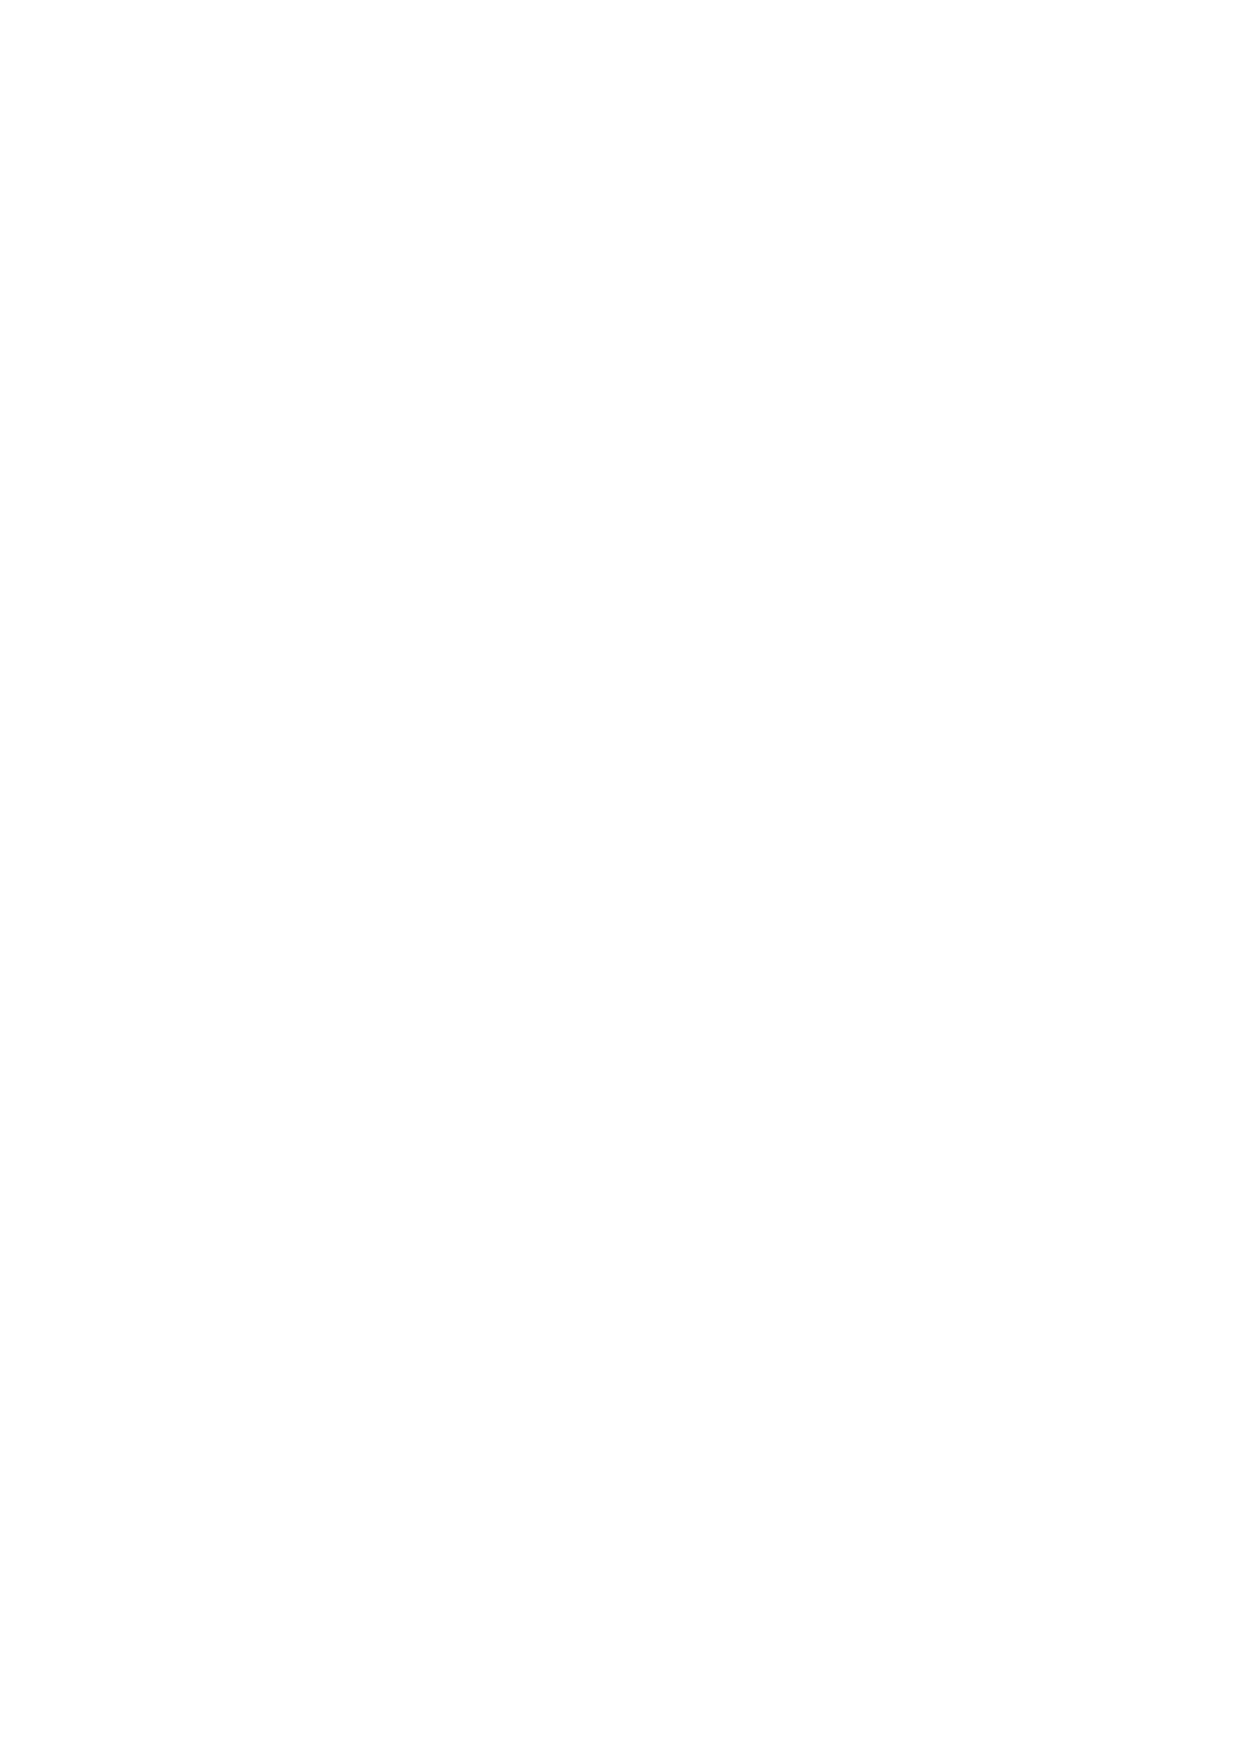
\includegraphics[width=0.55\textwidth]{figEa_MIS}%
\caption{\label{figEa_MIS}
Температурна залежність SCLC--струму ($V=0,4$~В)
$\gamma$--опроміненої МОН структури
%Au--SiO$_2$--Si
до УЗО.
Точки --- експеримент,
пряма --- лінійна апроксимація
}%
\end{figure}

Як відомо з літератури \cite{PersenkovBook}, при $\gamma$--опроміненні в системі Si--SiO$_2$
відбувається релаксація механічних напруг,
утворюються нові заряджені дефекти та заряджаються пастки, що вже були раніше.
Внаслідок цих процесів рельєф густини об'ємного заряду вирівнюється.
Вважається, що основними пастками, які захоплюють негативний заряд є центри на інтерфейсній межі розділу,
тоді як позитивний заряд накопичується на $E'$--центрах, $E'_\delta$-- центрах та трьох рівнях, пов'язаних
з напруженими зв'язками \cite{SiO2:Devine,SiO2:Lenahan}.
Проте при фотонному дефектоутворенні (використанні рентгенівських променів чи $\gamma$--квантів) останні рівні утворюються у значно меншій кількості, ніж два перших \cite{SiO2:Devine}.
Зауважимо, для досліджених зразків достатньо низькі температура та парціальний тиск кисню призводили до утворення тонких шарів окису кремнію, проте в літературі \cite{SiO2:Cantin} показано, що при цьому утворюються такі самі радіаційні дефекти, як і для прошарків більшої товщини.

Зазначимо, що ключовим фактором створення електричноактивних радіаційних дефектів у кремнієвих МОН структурах вважається вміст водню \cite{SiO2:Cantin}.
Плівки SiO$_2$ отримані термічним шляхом містять значну кількість атомів водню \cite{PersenkovBook}.
Утворення інтерфейсних рівнів пов'язується з розривом зв'язків $\equiv\!\text{Si}\!-\!\text{H}$ на межі Si--SiO$_2$ за наявності гарячих носіїв заряду \cite{SiO2:Mahapatra,SiO2:Esseni}.
Утворені ненасичені зв'язки $\equiv\text{Si}-$  діють як електронні пастки.
Загалом розрізняють дефекти подібного типу залежно від орієнтації кремнієвої підкладки, на якій вирощено шар окису.
Вважається, що на межі з кремнієм, орієнтованим у площині (111), з'являються $P_b$--центри, для (100) підкладки характерним є поява $P_{b1}$-- та $P_{b0}$--центрів \cite{SiO2:Rev}.
Ці центри хімічно ідентичні, проте характеризуються різною електричною активністю.
Крім того, при $\gamma$--опроміненні систем Si--SiO$_2$, вирощених на (111) підкладках, густина радіаційних поверхневих центрів вища ніж для (100) і досягає величини близько $10^{12}$~еВ/см для дози $10^{7}$~рад \cite{PersenkovBook}.

Відомо що при перевищенні дозою опромінення $\gamma$--квантами величини близько $5\cdot10^5$~рад у структурах Si--SiO$_2$ на основі кремнію з електронною провідністю спостерігається немонотонних розподіл інтерфейсних станів по енергії \cite{PersenkovBook}.
Згідно з даними роботи \cite{ParchSiO2} найбільша густина поверхневих станів спостерігається при
$E_c-(0,32\pm0,04)$~еВ, що збігається з отриманим значенням $E_x$,
Це свідчить, що проходження струму при малих прямих зміщеннях в досліджених структурах після опромінення зумовлене саме захопленням електронів $P_b$--центрами.
Накопичення від'ємного заряду на інтерфейсі також викликає збільшення висоти бар'єру,
що відображається у виявленому зменшенні ТЕ струму.
У літературі і раніше повідомлялося про зменшення струму внаслідок опромінення МОН--структур \cite{SiO2:Niu}.
Проте, як вже зазначалося, основною причиною зменшення ТЕ компоненти струму є дефектоутворення у приповерхневому шарі кремнію та відповідне зростання $n_\mathrm{id}$.

У результаті УЗО, як видно з рис.~\ref{figIV_MIS}, спостерігається збільшення струму, обмеженого просторовим зарядом.
Зокрема, при $t_\mathtt{UST}=60$~хв, цей струм перевищив термоемісійний у всьому дослідженому діапазоні напруг.
Параметри, отримані шляхом апроксимацій ВАХ, зведені в табл.~\ref{tabMIS}.
Виявлене збільшення $I_0$ свідчить, відповідно до формули~(\ref{eqIoSCLC}), про АІ зменшення концентрації $P_b$--центрів, а зростання $m_\mathrm{F}$ (або, що те саме, $T_c$) --- про звуження енергетичного розподілу відповідних рівнів.
З літератури \cite{SiO2:Takakura,SiO2:Wurzer} відомо, що відпал $P_b$--центрів відбувається внаслідок пасивації ненасичених зв'язків атомами водню.
Тобто отримані результати свідчать, що УЗО стимулює дифузію водню.
Загалом подібні процеси спостерігалися і раніше \cite{Ostap:SiO2,Ostap:PhotoLum,ostapenko1997}, проте в нашому випадку мова йде про АІ відпал радіаційних дефектів.


Як відомо \cite{Jafar}, випадок $m_\mathrm{F}=2$ відповідає наявності пасток з однаковим енергетичним рівнем.
Виявлене звуження енергетичного розподілу свідчить про певну вибірковість АІ процесів пасивації:
внаслідок УЗО атоми Н осідають переважно на зв'язки, яким відповідає цілком певне розташування рівнів у забороненій зоні.
На погляд автора, визначальним фактором того, які саме зв'язки будуть заповнені під час АІ відпалу є механічні напруги, неоднорідним чином розподілені на інтерфейсі.
Відомо, що дифузійна здатність домішок у напівпровідниках залежить від механічних напруг \cite{AZIZ2001}
(що може бути основною причиною переміщення водню в полі УЗ).
Відтак, від рівня деформації залежить ефективність АІ пасивації, а УЗО сприяє підвищенню однорідності структури.

Наслідком зменшення від'ємного заряду, накопиченого $P_b$--центрами, є часткове відновлення висоти бар'єру, що викликає зростання ТЕ струму --- див. дані для $I_s$ в табл.~\ref{tabMIS}.
Виявлене зменшення послідовного опору свідчить про частковий АІ відпал радіаційних дефектів у об'ємі напівпровідника.

Звільнені під час утворення $P_b$--центрів при $\gamma$--опроміненні атоми водню можуть
а)~взаємодіяти з іншими зв'язаними атомами Н на межі, викликаючи їхній відрив та утворення додаткових $P_b$--центрів \cite{SiO2:Devine};
б)~переміщуючись у кремнієву підкладку генерувати дефекти та деактивувати легуючу домішку \cite{SiO2:DiMaria};
б)~рухатися в об'єм діелектрика, де, за наявності гарячих носіїв заряду, призводити до появи $E'$--центрів (так званих, об'ємних пасток, bulk--oxide trap) внаслідок розриву зв'язків у системі $\equiv\!\text{Si}\!-\!\text{O}$ \cite{SiO2:Mahapatra,SiO2:Esseni}.
За своєю структурою $E'$--центри --- це вакансії кисню в SiO$_2$ \cite{SiO2:Takakura,SiO2:Devine},
які накопичують позитивний заряд.
Загальна концентрація цих дефектів при $\gamma$--опроміненні з дозою $10^{7}$~рад становить приблизно $10^{18}$~см$^{-3}$, проте по товщині оксидної плівки вони розподілені нерівномірно, найбільша кількість спостерігається біля межі з кремнієм \cite{PersenkovBook}.
Ці центри стабільні при кімнатній температурі \cite{SiO2:Mahapatra}, температура відпалу становить (200$\div$400)$^\circ$C.

Наявність розірваних зв'язків у об'ємі оксиду є причиною появи так званих напруго--індукованих струмів втрат (stress-induced leakage current, SILC) \cite{SiO2:Mahapatra,SiO2:DiMaria}.
 Саме цей струм реєструється в опромінених структурах при зворотному зміщенні (рис.~\ref{figIV_MIS},а та б).
Дійсно, відомо \cite{SiO2:Esseni,SiO2:DiMaria}, що SILC зумовлений тунелювання по пасткам (trap--assisted tunneling, ТАТ) .
Відповідно до \cite{TAT:Gilmore,TAT:GopalSST,TAT:Gopal}, польова залежність ТАТ--струму має вигляд:
\begin{equation}\label{eqIVTAT}
  I_R=I_{0,\mathrm{TAT}}\,(U_d+V_R)\exp\left(-\frac{R_\mathrm{TAT}}{F_m}\right),
\end{equation}
де
параметри $I_{0,\mathrm{TAT}}$ та $R_\mathrm{TAT}$ не залежать від напруги,
$I_{0,\mathrm{TAT}}$ пропорційний концентрації пасток,
$U_d$ --- висота бар'єру.
На рис.~\ref{figIV_MIS} наведено результати апроксимації експериментально отриманих зворотних гілок ВАХ згідно з формулою~(\ref{eqIVTAT}), що підтверджують припущення щодо природу цього струму.
Відхилення від очікуваної залежності при великих зміщеннях може бути зумовлене впливом послідовного опору.
Дані табл.~\ref{tabMIS} свідчать про низькотемпературний ($\sim$80$^\circ$C) АІ відпал радіаційно утворених пасток та зниження висоти бар'єру.
На нашу думку, відпал $E'$--центрів також зумовлений акустодифузією міжвузлових атомів, у даному випадку  кисню.

Збільшення прямого струму та зменшення зворотного в результаті УЗО викликає збільшення коефіцієнта випрямлення
$K_\mathrm{RECT}$, який суттєво зменшився в результаті $\gamma$--опромінення.
У табл.~\ref{tabMIS} наведено значення цієї величини при напрузі 0,5 В.
Дані свідчить, що УЗО при температурах, близьких до кімнатних, здатна частково відновлювати характеристики радіаційно--деградованих  МОН  пристроїв.







\section*{Висновки до розділу \ref{Ch_UST_MW}}
\addcontentsline{toc}{section}{Висновки до розділу \ref{Ch_UST_MW}}
  \begin{enumerate}[leftmargin=0cm,itemindent=3em]
\item Експериментально досліджено вплив мікрохвильового опромінення на параметри точкових дефектів (поперечний переріз захоплення електронів,
розташування енергетичних рівнів у забороненій зоні) в монокристалах $n$--6$H$--SiC, $n$--GaAs та епітаксійних структурах на основі арсеніду ґалію.


\item Показано, що у приповерхневому шарі присутні центри захоплення носії заряду, пов'язані з власними дефектами вакансійного типу.
Виявлені зміни параметрів пасток обумовлені індукованим мікрохвильовим випроміненням
збільшенням кількості міжвузлових атомів.
Показано, що наявність стискуючих напруг у приповерхневому шарі сприяє перетворенню дефектних комплексів внаслідок високочастотного опромінення.

     \item Вперше експериментально досліджено вплив ультразвукової обробки на параметри структур Au--TiB$_x$--$n$--$n^+$--GaAs з контактом Шотткі залежно від частоти та інтенсивності акустичних хвиль.
%Виявлено, що вплив ультразвуку на зворотні гілки ВАХ значно суттєвіший ніж на прямі.
 Експериментально встановлено, що при допороговій інтенсивності (менше 2,5~Вт/см$^2$) характер ультразвукового впливу на зворотний струму залежить від механізму перенесення заряду:
  якщо домінуючим механізмом є тунельний, то УЗО викликає збільшення зворотного струму, якщо термоемісійний --- зменшення.
  Показано, що причиною  виявлених ефектів при допороговій інтенсивності УЗО
  може бути акусто--стимульована дифузія точкових дефектів, тоді як зростання зворотного струму при надпороговій  інтенсивності зумовлене акусто--індукованою генерацією дефектів.
 Виявлено, що зі збільшенням частоти ультразвукової обробки інтенсифікуються процеси перебудови дефектів, які забезпечують проходження тунельного струму.

\item Показано, що ультразвукова обробка здатна викликати зменшення розкиду параметрів і підвищення однорідності характеристик напівпровідникових пристроїв, створених в єдиному технологічному процесі.

\item %Досліджено вплив ультразвукової обробки на парметри структур метал--окис--напівпровідник.
   Виявлено можливість низькотемпературного відпалу радіаційних дефектів у системі Si--SiO$_2$.
   Показано, що акусто--індукований відпал зумовлений дифузією міжвузлових атомів.
 Виявлено, що ультразвукова обробка сприяє звуженню енергетичного спектра радіаційно--індукованих пасток
на інтерфейсі системи    Si--SiO$_2$.


\end{enumerate}	



Основні результати даного розділу представлені в роботах \cite{Olikh:SPQEO2003,Olikh:PJE2004,Olikh:PhChOM2005,Olikh:PZTF2006,Gorb2010,
3Tomsk,50IUFFC,9APTTE,ICU2007GA,6DrogGorb}.



%\cite{PersenkovBook}
%При гамма--опроміненні релаксація механічних напруг в системі Si--SiO$_2$:
%частина дірок, що утворилася при іонізації захоплюється на рівні напружених зв'язків, що призводить до їх розриву
%термічно отримані плівки SiO$_2$ поліморфні,
%%містять велику кількість водню
%
%%Е' центри (пастки дірок) розподілені нерівномірно, найбільша концентрація біля границі з Si.
%%загальна концентрація при 1е7 рад ---  близько 1е18 см-3.
%
%тривалентний кремній --- донороподібний центр,
%відповідає за додатній заряд, який накопичується в об'ємі при опроміненні
%
%%при опроміненні Si--SiO$_2$ утворюються нові заряджені дефекти та заряджаються пастки,
%%що вже були,
%%рельєф густини об'ємного заряду вирівнюється
%
%швидкі поверхневі стани розташовані в приповерхневому шарі напівпровідника,
%повільні --- в приграничній області оксиду.
%
%%густина утворених поверхневих станів при гамма--опроміненні найбільша при (111), найменша (100),
%%при 1е7 рад порядку 1е12 еВ/см2
%
%кореляція між густиною швидких поверхневих станів Nss та пасткових центрів в об'ємі SiO$_2$ No
%Nss=3.75t-6 см/еВ No,
%а отже однакова причина утворення дефектів:наявність напружених валентних зв'язків між атомами та їх розрив в результаті іонізації.
%
%%при опроміненні гамма--квантами найбільша густина станів в околі Ес-(0,3-0,4)еВ (для електронного, для діркового не так),
%%причому така нерівномірність спостерігається лише при перевищенні дозою порогу близько 5е5 рад.
%
%швидкість поверхневої рекомбінації визначається густиною поверхневих станів
%s~Nss
%
%в об'ємі напівпровідника час життя змінюється мало при гамма-опроміненні, в приповерхневому шарі зменшується
%
%%\cite{ParchSiO2}
%%часткова компенсація напівпровідникової підкладинки в процесі радіаційного дефектоутворення
%%гамма--кванти, до 2е7 рад, максимум спектра поверхневих станів Ес-(0,32+-0,04) ев, що характерно для високих доз -- див попередню
%%
%%електронне опромінення (n-тип, (100)) --- максимум густини поверхневих станів Ес-0,3 еВ \cite{LaiSiO2}
%
%
%
%%Interface trap (Nit) утворюються внаслідок розриву зв'язків $\equiv\!\text{Si}\!-\!\text{H}$ на інтерфейсі Si--SiO$_2$,
%%в результаті утворюються $\equiv\text{Si}-N_\text{iT}$, які реєструються як Pb центри.
%%Звільнені атоми водню рухаються в об'єм діелектрика.
%%За наявності гарячих носіїв заряду при цьому генеруються bulk--oxide trap Not внаслідок розриву $\equiv\!\text{Si}\!-\!\text{O}$.
%%Розірвані зв'язки $\equiv\!\text{Si}\!-\!\text{O}$ в об'ємі оксиду викликають появу stress-induced leakage current (SILC).
%%However, unlike $\equiv\!\text{Si}\!-\!\text{H}$  bonds, broken $\equiv\!\text{Si}\!-\!\text{O}$ bonds are not known to recover
%%at room temperature after the stress is removed.
%%В роботі пропонується, що $\equiv\!\text{Si}\!-\!\text{H}$ bonds are broken by holes (and not by electrons). \cite{SiO2:Mahapatra}
%
%
%%Гарячі електрони ведуть до звільнення водню з інтерфейсу Si--SiO$_2$,
%%міграція Н в оксиді викликає появу bulk--oxide trap.
%%Механізм SILC --- trap--assisted tunneling
%%The results reported so far demonstrate that in the channel hot electron stress conditions there is no correlation between and SILC generation.
%%В самій роботі Nit generation is evidently related to stress-induced leakage current (H/D) release \cite{SiO2:Esseni}
%%
%%SILCs  (This  phenomenon  is  often  referred  to  as  trap-assisted  tunneling ) can  be  best  explained  by  the generation  of  neutral  electron  traps  in  the  oxide  layer.
%%These  studies  have  directly  shown  the  relationship  of SILCs  to  the  trap  creation  phenomenon.
%%Trapped  holes  or  sites  produced by  trapped-hole  annihilation  by  free  electrons  will  be demonstrated  not  to  contribute  to  SILC  for  most  stressing conditions.
%%Since  the  oxide  deterioration  producing  SILC  will  be shown  here  to  be  caused  by  electron  heating  in  the  oxide layer,
%%oxide  defect  formation  due  to  hot  carriers  will  be briefly  reviewed.
%%The  production  of  interface  states or  traps by  the  annihilation  of  trapped  holes  and/or  their  presence  is
%%one  component  of  the  oxide  degradation  process.
%%The other  component  is  due  to  the  trap  creation  process  also  caused by  hot  electrons.
%%  Also, the  most  significant  component  contributing  to  the  SILC  in the  experiments  discussed here  appears to  be due  to  the  generation  of  the  neutral-electron  traps,  not  the  interface  states and/or  anode positive  charge.
%%Also,  generation--recombination  sites  and boron  deactivation  can be produced  in  the Si  substrate by  the hydrogen.
%%However,  during  trap  creation,  many  different  defect  sites  with  different  processing  dependencies  from  one wafer  run  to  another  can  occur.  These  defects  include  interface  states, generation-recombination  centers  in  the  Si  substrate,  neutral  electron  traps  in  the  oxide  bulk  distributed  away  from  the  cathode/oxide  interface,  and positively  charged  oxide  sites  (mostly  <<slow  states>> )  near the  anode/oxide  interface.\cite{SiO2:DiMaria}
%
%%На границі з (111) --- Pb центр,
%%на границі з (100) --- Pb1 та Pb0.
%%центри хімічно ідентичні, різна електрична активність (Pb1, здається не активний)
%%взагалі робота --- огляд.. там багато всякого про інтерфейсні рівні \cite{SiO2:Rev}
%
%%Опромінення гамма--квантами, доза 1е6,
%%утворилися нові інтерфейсні рівні (порядку 3е10 см-2).. головна ідея -- при прикладенні напруги в опромінених структурах генеруються більше пасток \cite{AASSIME1997}
%
%%тонкі (20--40 ангстрем) шари , опромінення х-променями (10 кев), утворюються такі самі дефекти (Е' (позитивно заряджені вакансії кисню) та два типи Pb, бо (100) пластинки)
%%that one key parameter for the moddication of the electrically  active  defects  in  MOS  structures  is their hydrogen content \cite{SiO2:Cantin}
%
%%опромінення протонами (еквівалентна доза гамма--квантів близько 1е6) --- зміни струмів різних (там транзистор) можуть бути і від'ємні після опроміненя
%%is  shown  to be  a result  of  the increase  in  fixed oxide  charge  and  surface  trap  densities,  in combination with the different SRH  recombination rate limiting
%%mechanisms in the presence of high density surface traps \cite{SiO2:Niu}
%
%%огляд радіаційних дефектів в SiO2:
%%пастки, які захоплюють позитивний заряд--- відпалюються при температурах 200--400 градусів цельсію
%%Е' центр (вакансія кисню) --- основний,
%%$E'_\delta$ (комплекс вакансія кисню--кремній), тяжко утворюється при дії фотонів (гамма та Х)
%%три пастки пов'язані з напруженими зв'язками
%%негативний заряд
%%Pb центри (причому звільнені атоми водню можуть взаємодіяти і іншими, ще зв'язаними, і відривати їх також)
%%як не дивно, знову вакансії кисню
%%we generally expect the neutral oxygen-vacancy to be a hole trap, it may also trap electrons leading  to a negatively charged state in the SiO2  bandgap
%%about 1  eV below the conduction band edge \cite{SiO2:Devine}
%
%%decrease of base current during annealing. We  found that two mechanisms
%%are responsible for annealing: the recombination  of charges and
%%the bonding of hydrogen atoms on interface traps.
%%процеси з двома енергіями активації -- 0,23 ев та 0,046ев
%%As  the  Shockley-Read-Hall  current  is  proportional to the
%%density of  interface traps,  the decrease of  the base current
%%is proportional to  the  density of  the  annealed interface traps. \cite{SiO2:Wurzer}
%
%%Ще одна робота про результат опромінення: переважно Е', Pb (або два варіанти для 100) все повторюється..
%%і те, що Pb амфотерний (може захоплювати і дірки, якщо його рівень в нижній половині забороненої зони)\cite{SiO2:Lenahan}
%
%%It is well established nowadays that one of the main hole trapping centres responsible for irradiation-induced positive
%%charge is the E'-centre. Electron spin resonance (ESR)
%%studies have revealed that the E'-centre is a defect resulting
%%from an oxygen vacancy in SiO2. A direct correlation has been
%%established between the annealing of the oxide-trapped charge.
%%The key SiO2/Si interface defect is called Pb-centre and
%%corresponds to a silicon dangling bond at the interface, back-
%%bonded by three other silicon atoms . Passivation of these dangling bonds (DBs) occurs
%%through binding with hydrogen.
%%From this result it is concluded that the degradation
%%and recovery of the device performance are mainly caused by
%%trapped-oxide charge
%%Вираз для струму, пов'язаного з поверхневою рекомбінацією, близький до того, що використовували ми
%%\cite{SiO2:Takakura}
%
%%залежність дифузійної здатності від механічних напруг \cite{AZIZ2001}
%%
%%\cite{Ostap:SiO2} стан границі Si--SiO2, підсилення дифузії водню
%%\cite{Ostap:PhotoLum,ostapenko1997} підсилення дифузії водню




%\chapter{Оформление различных элементов} \label{chapt1}
%
%\section{Форматирование текста} \label{sect1_1}
%
%%\arabic{\curtextsize}
%
%Мы можем сделать \textbf{жирный текст} и \textit{курсив}.
%
%%\newpage
%%============================================================================================================================
%
%\section{Ссылки} \label{sect1_2}
%Сошлёмся на библиографию.
%\cite{Olikh:Visn2003,Olikh:SPQEO2003,Olikh:SEMT2004,Olikh:PJE2004,Olikh:PhChOM2005,
%Olikh:PZTF2006,Olikh:MRS2007a,Olikh:SEMT2007,Olikh:Visn2007,Olikh:FTP2009,Olikh:SPQEO2010,Gorb2010,
%Olikh:UPJ2010,Olikh:SEMT2011,Olikh:FTP2011,Olikh:2013IEEE,Olikh:UPJ2013,Olikh:FTP2013,Olikh:SEMT2013,
%Olikh:UPJ2014,Olikh:Ultras,OlikhJAP,Olikh:Rev,Olikh:Ultras2016,Olikh2016JSem,Olikh2018JAP,
%1UNCPS,3Tomsk,1SEMST,50IUFFC,9APTTE,2005IUS,ICU2007SC,ICU2007GA,2007MRS,3UNCPS,6DrogGorb,6Drog,
%12IvFr,4UNCPS,4Kremen,7Drog,5UNCPS,2012Ternop,14Plivk,8Drog,2013Buk,6UNCPS,2014IUSOl,2014IUS,6SEMST,
%2015ICU,6CPFCS,7UNCPS,2017MEICS}
%Одна ссылка: \cite[с.~54]{OlikhJAP}.
%\nocite{*}


%\include{Dissertation/StatsAndAbst}
%\include{Dissertation/stats}



%\include{Dissertation/conclusion}      % Заключение
%\include{Dissertation/dictionary}      % Словарь терминов
\clearpage                                  % В том числе гарантирует, что список литературы в оглавлении будет с правильным номером страницы
%\hypersetup{ urlcolor=black }               % Ссылки делаем чёрными
%\providecommand*{\BibDash}{}                % В стилях ugost2008 отключаем использование тире как разделителя
%\urlstyle{rm}                               % ссылки URL обычным шрифтом
\ifdefmacro{\microtypesetup}{\microtypesetup{protrusion=false}}{} % не рекомендуется применять пакет микротипографики к автоматически генерируемому списку литературы
\insertbibliofull                           % Подключаем Bib-базы
\ifdefmacro{\microtypesetup}{\microtypesetup{protrusion=true}}{}
%\urlstyle{tt}                               % возвращаем установки шрифта ссылок URL
%\hypersetup{ urlcolor={urlcolor} }          % Восстанавливаем цвет ссылок
      % Список литературы
%\include{Dissertation/lists}           % Списки таблиц и изображений (иллюстративный материал)
%\include{Dissertation/appendix}        % Приложения

\end{document}
